%\documentclass[titlepage,twoside,openright,report]{jsbook}
\documentclass[titlepage,twoside,openright]{jsreport}
%\usepackage{thesisj}
\usepackage[dvipdfmx]{graphicx,xcolor}
\usepackage{subcaption}
\usepackage{amsmath,amssymb}
\usepackage{booktabs}
\usepackage{tabularx}
\usepackage{url}
\usepackage[dvipdfmx]{hyperref}
\usepackage{multirow}
\usepackage[cc]{titlepic}
\usepackage{fancyhdr}
\usepackage{makeidx}
\usepackage{braket}
%\bibliographystyle{jplain} % sorted by abc
\bibliographystyle{junsrt} % sorted by appearance

\makeatletter
\renewcommand{\chapter}{%
  \if@openleft\cleardoublepage\else
  \if@openright\cleardoublepage\else\clearpage\fi\fi
  \global\@topnum\z@
  \secdef
      {\@omit@numberfalse\@chapter}%
      {\@omit@numbertrue\@schapter}}
\makeatother

\pagestyle{fancy}
\lhead[\thepage]{\rightmark}
\chead[]{}
\rhead[\leftmark]{\thepage}
\lfoot[]{}
\cfoot[]{}
\rfoot[]{}
\renewcommand{\headrulewidth}{1pt}
\renewcommand{\footrulewidth}{0pt}
%\fancyhead{}
%\renewcommand{\chaptermark}[1]{\markboth{第\ \thechapter\ 章\,\, #1}{}}
%\fancyhead[RO]{{\small \rightmark}}
%\fancyhead[LE]{{\small \leftmark}}
%\renewcommand{\headrulewidth}{0pt}
%\fancyfoot{}
%\fancyfoot[LE,RO]{{\small \thepage}}
%\cfoot{}
% modify the width of caption
\setlength{\captionmargin}{50pt}

\makeindex
\title {\Huge{MAIKo TPC を用いた${}^{12}\rm{C}(n,n'){}^{12}\rm{C}(0_{2}^{+})$の}\\\Huge{散乱断面積の測定}}
\author{\Large{京都大学大学院 理学研究科}\\
  \Large{物理学・宇宙物理学専攻}\\
  \Large{物理学第二教室}\\
  \Large{原子核・ハドロン物理学研究室}\\
  \LARGE{土井 隆暢}}
\date{}
\titlepic{
\includegraphics[width=0.5\columnwidth]{eps/E-C.eps}}


\begin{document}
\maketitle
%\frontmatter
\documentclass[./master]{subfiles}
\begin{document}
\begin{abstract}
  宇宙元素合成において,${}^{12}\mathrm{C}$原子核は3つの$\alpha$粒子から直接合成される(トリプルアルファ反応).
  トリプルアルファ反応では主に3$\alpha$崩壊閾値近傍に位置する3$\alpha$共鳴状態である$0_2^+$ (\SI{7.65}{\mega\electronvolt})
  状態 (Hoyle状態) を経由する.大半の$0_2^+$状態は3つの$\alpha$粒子に崩壊するが,稀に$\gamma$線を放出して脱励起することで,
  安定した${}^{12}\mathrm{C}$原子核となる.
  トリプルアルファ反応は${}^{12}\mathrm{C}$より重い元素を合成するための戸口反応であり,
  宇宙元素合成において最も重要な原子核反応の一つである.
  しかし,$\rho = \SI{e6}{\gram\per\centi\metre}$のような高密度環境下では,
  $\gamma$崩壊に加え,他の粒子との非弾性散乱による脱励起が増加しトリプルアルファ反応を劇的に促進することが指摘されている.
  特に中性子は電荷を持たずクーロン力の効果を受けないため,
  脱励起を促進する効果が大きいと考えられている.

  脱励起の反応率の計算には,${}^{12}\mathrm{C}$が中性子との散乱により
  ${}^{12}\mathrm{C} (0_2^+)$へ励起する断面積が必要となる.
  特に,$0_2^+$状態へ励起させることができる中性子エネルギーの
  閾値付近 ($E_{\text{lab}} = \SI{8.3}{\mega\electronvolt}$) における断面積が重要となる.
  しかし,$E_{\text{lab}} = \SI{8.3}{\mega\electronvolt}$付近におけるg.s. $\rightarrow$ $0_2^+$状態の
  断面積は測定されていない.
  そこで,我々は中性子ビームを用いて${}^{12}\mathrm{C} (0_2^+)$へ励起し,
  ${}^{12}\mathrm{C} (0_2^+)$状態から崩壊した3つの低エネルギー$\alpha$粒子を測定することで,
  崩壊元の状態を特定しg.s. $\rightarrow$ $0_2^+$状態反応の断面積を決定することを計画している.
  このためには,3つの$\alpha$粒子を全て測定するための大きな立体角を多い,
  低エネルギー$\alpha$粒子を効率的に検出することのできる検出器が必要となる.
  この要求を満たす検出器にMAIKo TPC がある.

  MAIKo TPC では,検出器のガス中を通過した荷電粒子のトラックが画像として検出される.
  検出器中でのトラックの長さと方向から荷電粒子のエネルギーと運動量を決定するため,
  画像から$\alpha$粒子のトラックを正しく抽出することが必要となる.
  MAIKo TPC で検出されるトラックの分解能が検出ガスの種類によって大きく変わる.
  そこで,どのような検出ガスが測定に適しているか,
  その時の検出効率は十分か,$0_2^+$状態を識別するのに十分な分解能が達成できるかを
  現実的な実験条件を仮定して検討する必要がある.

  本研究では,MAIKo TPC で用いる検出ガスの候補を複数選出し,
  $\alpha$線源を用いた性能試験を行った.
  また,それらの検出ガスについて,
  中性子との散乱で${}^{12}\mathrm{C}$原子核が3つの$\alpha$粒子に崩壊するイベントの画像を,
  シミュレーションによって生成した.
  さらに,シミュレーションで生成した画像に対して解析を行い,
  検出効率,エネルギー分解能,角度分解能を評価した.
  シミュレーションによる検討の結果,
  \SI{100}{\hecto\pascal}の\isoButaneHydro を検出ガスに用いれば,
  計画中の実験を遂行するのに十分な検出効率および${}^{12}\mathrm{C}$の励起エネルギー分解能を実現できることが推定された.
\end{abstract}
\end{document}

\pagenumbering{Roman}
\tableofcontents
%\pagenumbering{roman}
%\listoffigures
%\listoftables
\newpage
%\mainmatter
\pagenumbering{arabic}
\documentclass[../master]{subfiles}
\begin{document}

\chapter{はじめに}
\section{宇宙での元素合成}
\label{seq::nucleaosynthesis}
身の回りには多種多様な物質が存在しており,
これらの物質は全て原子から構成されている.
現在の地球には水素(原子番号1)からウラン(原子番号92)までの元素が天然に存在してる.
原子は更に小さい原子核と電子から構成されており,原子核は陽子と中性子で構成されることが知られている.
原子核に含まれる陽子の数が元素の原子番号となる.
現在までに天然と人工を合わせて118種類の元素が確認されている.
しかし,原始の宇宙では物質は存在せず,エネルギーの塊であったと考えられている.
宇宙が膨張し温度が下がるにしたがって,陽子と中性子が生成された.
その後,原子核反応を起こすことで様々な原子核が合成された.
宇宙の初期には,水素とヘリウムと僅かな軽元素しか合成されなかった考えられている.
これは,質量数 ($A$) が5と8の原子核に安定な原子核が存在しないことに由来する.
初期の宇宙では陽子や中性子が融合して原子核が大きくなっていくが,
$A = $5と8の原子核が生成してもすぐに$A = $4 以下の軽い原子核に分裂してしまうのである.

%ヘリウムに比べて水素の方が多いため,水素を主成分とする恒星しか存在しなかったと考えられる.
宇宙に存在する元素のうち殆どが水素であるため,生まれたばかりの恒星は水素を主成分とする.
重力により収縮し中心温度が\SI{e7}{\kelvin}を超えると,
陽子(水素)同士が連鎖的に反応するようになる (ppチェイン).
ppチェインでは図\ref{fig::pp_chain}に示した3つの系列が重要とされる.
%chain~1 では3つの陽子から1つの${}^{3}\mathrm{He}$が形成され,
%2つ${}^{3}\mathrm{He}$から1つの$\alpha粒子と2つの陽子が生成される.
chain~1 では合計6つの陽子から1つの$\alpha$粒子と2つの陽子が生成される.
chain~2, 3 では合計で4つの陽子と1つの$\alpha$粒子から2つの$\alpha$粒子が生成される.
%chain~2, 3 では$A = $7
どの系列も最終的に4つの陽子から1つの${}^{4}\mathrm{He}$原子核($\alpha$粒子)が生成される.
ppチェインのように粒子(陽子や$3{}^{3}\mathrm{He}$など)が順番に一つずつ原子核に吸収される反応では,
$A = $8の壁を超えることはできない.
この壁を超えるためには$A = $4以下の原子核から$A = $9以上の原子核が直接生成されなければならない.
%\begin{gather}
%  {\rm p}({\rm p},\beta^{+}\nu){\rm d}({\rm p},\gamma){}^{3}{\rm He}({}^{3}{\rm He},2{\rm p})\alpha\label{eq::pp1}\\
%  {\rm p}({\rm p},\beta^{+}\nu){\rm d}({\rm p},\gamma){}^{3}{\rm He}(\alpha,\gamma){}^{7}{\rm Be}({\rm e}^{-},\nu){}^{7}{\rm Li}({\rm p},\alpha)\alpha\label{eq::pp2}\\
%  {\rm p}({\rm p},\beta^{+}\nu){\rm d}({\rm p},\gamma){}^{3}{\rm He}(\alpha,\gamma){}^{7}{\rm Be}({\rm p},\gamma){}^{8}{\rm B}(\beta^{+}\nu){}^{8}{\rm Be}(\alpha)\alpha\label{eq::pp3}
%\end{gather}
%\begin{gather}
%  \begin{array}{llll}
%    {\rm p} + {\rm p} \rightarrow & {\rm d} + \beta^{+} + \nu & &\\
%    & {\rm d} + {\rm p} \rightarrow & {}^{3}{\rm He} + \gamma &\\
%    & & {}^{3}{\rm He} + {}^{3}{\rm He} \rightarrow & {\rm \alpha} +2{\rm p}
%  \end{array}\label{eq::pp1}\\  
%  \begin{array}{llllll}
%    {\rm p} + {\rm p} \rightarrow & {\rm d} + \beta^{+} +\nu & & & &\\
%    & {\rm d} + {\rm p} \rightarrow & {}^{3}{\rm He} + \gamma & & &\\
%    & & {}^{3}{\rm He} + \alpha \rightarrow & {}^{7}{\rm Be} & &\\
%    & & & {}^{7}{\rm Be} + {\rm e}^{-} \rightarrow & {}^{8}{\rm Li} + \nu &\\
%    & & & & {}^{7}{\rm Li} + {\rm p} \rightarrow & \alpha + \alpha
%  \end{array}\label{eq::pp2}\\
%  \begin{array}{lllllll}
%    {\rm p} + {\rm p} \rightarrow & {\rm d} + \beta^{+} + \nu & & & & &\\
%    & {\rm d} + {\rm p} \rightarrow & {}^{3}{\rm He} + \gamma & & & &\\
%    & & {}^{3}{\rm He} + \alpha \rightarrow & {}^{7}{\rm Be} + \gamma & & &\\
%    & & & {}^{7}{\rm Be} + {\rm p} \rightarrow & {}^{8}{\rm B} + \gamma & &\\
%    & & & & {}^{8}{\rm B} \rightarrow & {}^{8}{\rm Be} + \beta^{+} + \nu &\\
%    & & & & & {}^{8}{\rm Be} \rightarrow & 3\alpha
%  \end{array}\label{eq::pp3}
%\end{gather}
\begin{figure}
  \centering
  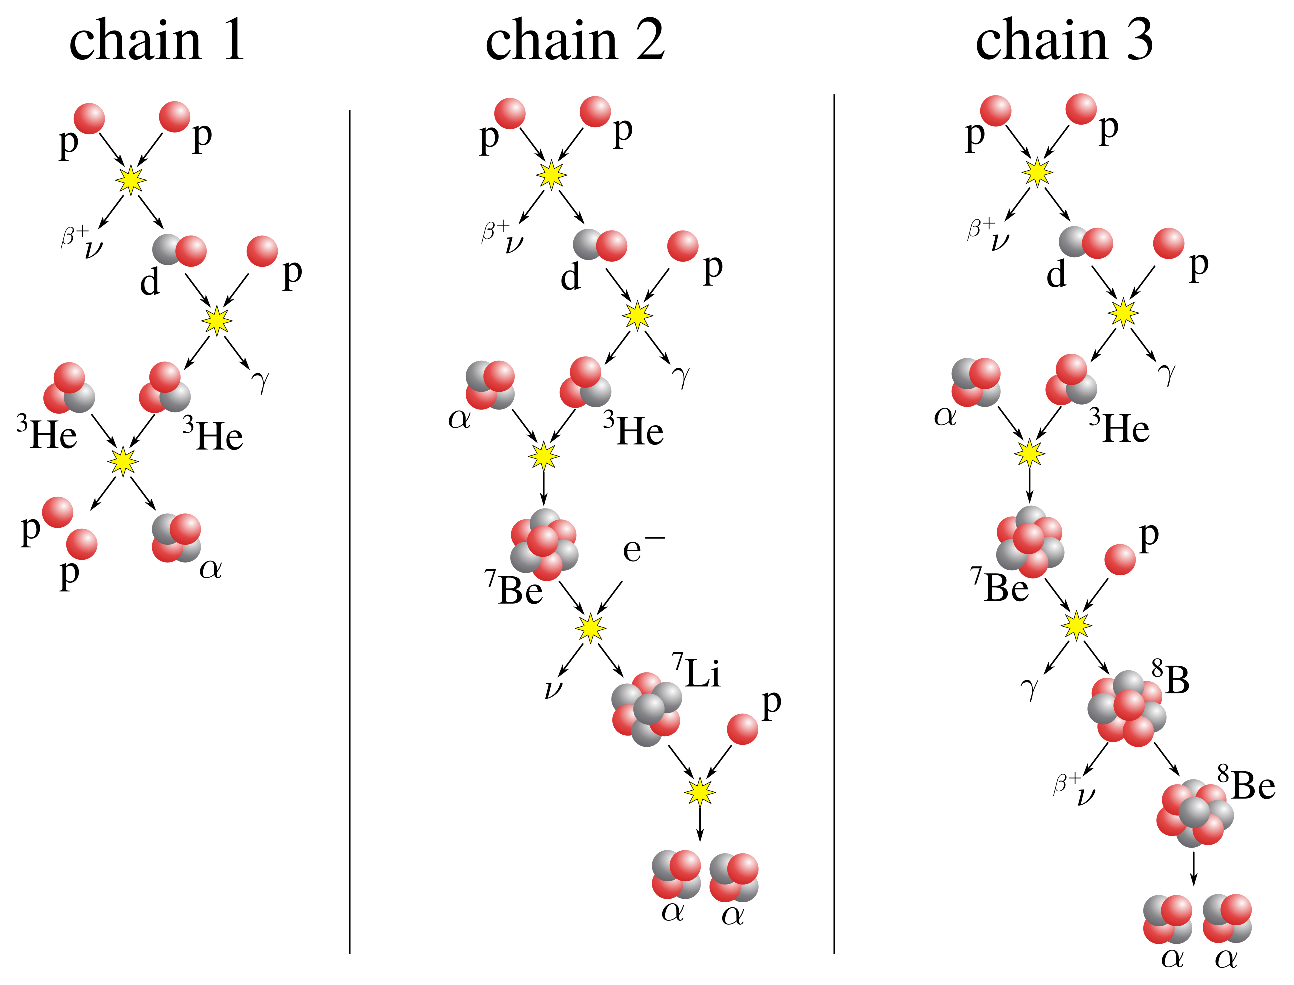
\includegraphics[clip, width=0.9\columnwidth]{pp_chain.eps}
  \caption{代表的なpp チェイン.pp チェインでは4つの陽子から1つの$\alpha$粒子が生成される.}
  \label{fig::pp_chain}
\end{figure}

ppチェインにより$\alpha$粒子が十分に生成された恒星では水素よりも重い$\alpha$粒子が
より恒星の中心に集まり$\mathrm{He}$コアを生成する.
$\mathrm{He}$コアが重力により圧縮され温度が約\SI{e8}{\kelvin}に達するとヘリウム燃焼が始まる.
$\mathrm{He}$コアには十分な量の$\alpha$粒子が存在するため,
図\ref{fig::triple_alpha}のように2つの$\alpha$粒子から2$\alpha$クラスター状態である${}^{8}\mathrm{Be}$が合成され,
さらに,${}^{8}\mathrm{Be}$が崩壊するより早くもう1つの$\alpha$粒子が
融合して${}^{12}\mathrm{C}$の励起状態 (${}^{12}\mathrm{C}^{*}$) が生成される反応が起こる.
このときに作られる${}^{12}\mathrm{C}^{*}$の多くはFred Hoyle が予言した$3\alpha$粒子の
共鳴状態 (Hoyle状態,$E_{x} = \SI{7.65}{\mega\electronvolt}$,$0_{2}^{+}$)~\cite{hoyle_state}となる.
${}^{12}{\rm C} (0_2^+)$が$\gamma$線を放出し脱励起することで安定な${}^{12}\mathrm{C}$原子核になる
 (図\ref{fig::triple_alpha}~左) .
この3つの$\alpha$粒子から${}^{12}\mathrm{C}$が直接合成される反応はトリプルアルファ反応と呼ばれる.
トリプルアルファ反応が恒星中で起こることで$A = $4から$A = $12へと直接移るため,$A = $5, 8の壁を乗り越えることができ,
さらに重い$\mathrm{O}$や$\mathrm{Si}$などの合成へ進んでいく.
そのため,トリプルアルファ反応は宇宙元素合成において重要な原子核反応の1つである.
%\begin{equation}
%  \begin{array}{llll}
%%  \alpha(\alpha,\gamma){}^{8}{\rm Be}(\alpha,{}^{12}{\rm C}^{{\rm Hoyle}})
%%  \alpha(\alpha,\gamma){}^{8}{\rm Be}+\alpha\rightarrow{}^{12}{\rm C}^{{\rm Hoyle}}\label{eq::triplealpha}
%  %あとで矢印の絵を書こうかな
%    \alpha + \alpha \rightarrow & {}^{8}{\rm Be} & & \\
%    & {}^{8}{\rm Be} + \alpha \rightarrow & {}^{12}{\rm C}^{{\rm Hoyle}} &\\
%    & & {}^{12}{\rm C}^{{\rm Hoyle}} \rightarrow & {}^{12}{\rm C} + \gamma
%  \end{array}\label{eq::triplealpha}
%\end{equation}
\begin{figure}
  \centering
  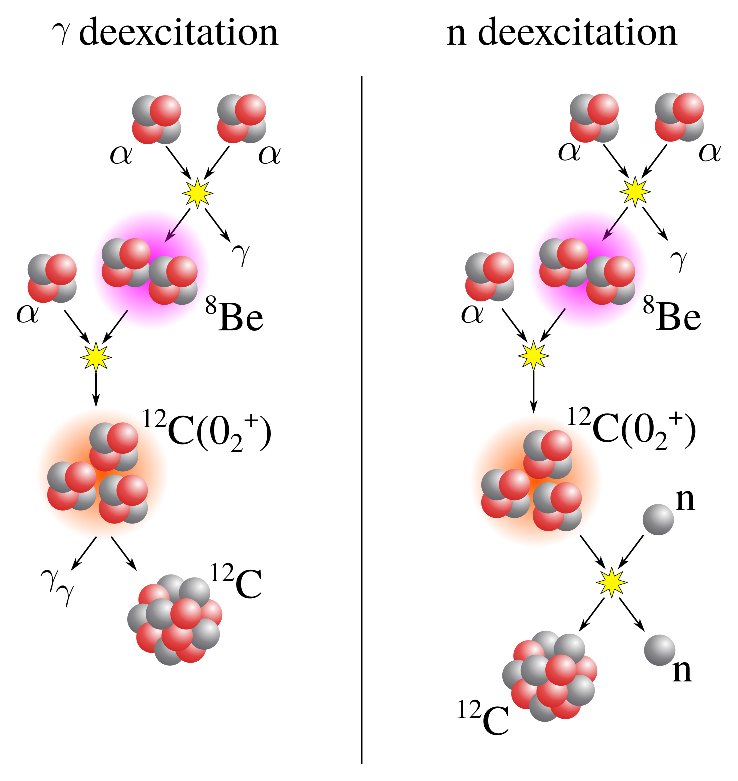
\includegraphics[clip, width=0.7\columnwidth]{triple_alpha.eps}
  %  \caption{トリプルアルファ反応.3つの$\alpha$粒子が反応し1つの${}^{12}{\rm C}$が生成される.}
  \caption[トリプルアルファ反応.]{トリプルアルファ反応.
    左は$\gamma$線を放出して脱励起するルート,右は中性子との非弾性散乱により脱励起するルートを表す.}
  \label{fig::triple_alpha}
\end{figure}

\section{高密度環境下でのトリプルアルファ反応}
\label{seq::triplealphareaction}
通常,トリプルアルファ反応で生成された$3\alpha$共鳴状態は図\ref{fig::triple_alpha} の左のように
$\gamma$線を放出することによって脱励起し,${}^{12}\mathrm{C}$の基底状態 (g.s.) になる.
近年,高密度環境下では$\gamma$線による脱励起以外に,
図\ref{fig::triple_alpha}~(右) のように粒子(陽子,中性子,$\alpha$粒子など)との
非弾性散乱による脱励起の反応率が増加することが指摘されている~\cite{hotdensemedium}.
これにより$0_2^+$状態からg.s.や$2_{1}^{+}\ (E_{x} = \SI{4.44}{\mega\electronvolt})$ への脱励起が増加し,
トリプルアルファ反応が劇的に促進されると考えられている.
粒子の中でも中性子は電荷を持っておらず,クーロン斥力を受けずに反応することができるため,
特にトリプルアルファ反応を促進する効果が大きい.

%\begin{equation}
%  \begin{array}{llll}
%    \alpha + \alpha \rightarrow & {}^{8}{\rm Be} & &\\
%    & {}^{8}{\rm Be} + \alpha \rightarrow & {}^{12}{\rm C}^{{\rm Hoyle}} &\\
%    & & {}^{12}{\rm C}^{{\rm Hoyle}} + {\rm X} \rightarrow & {}^{12}{\rm C} + {\rm X'}
%  \end{array}\label{eq::triplealpha_particle}
%\end{equation}

%\begin{figure}
%  \centering
%  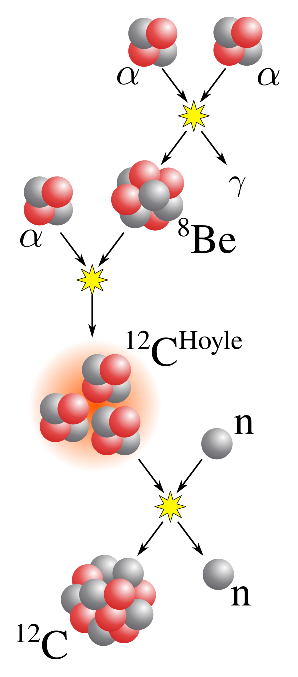
\includegraphics[clip, width=0.5\columnwidth]{triple_alpha_n.eps}
%  \caption[粒子との散乱により脱励起するトリプルアルファ反応.]{粒子との散乱により脱励起するトリプルアルファ反応.
%  この図では中性子と散乱する場合を表している.}
%  \label{fig::triple_alpha_n}
%\end{figure}%

%${}^{12}\mathrm{C}$と中性子の反応レートは
${}^{12}\mathrm{C}(0_2^+)(\mathrm{n}',\mathrm{n}){}^{12}\mathrm{C}$反応の
体積当たりの反応率は
\begin{equation}
  r = N_{\text{n}}N_{{}^{12}\mathrm{C}}\braket{\sigma v}% \si[per-mode=reciprocal]{\per\cubic\centi\metre\per\second}
  \label{eq::r}
\end{equation}
で与えられる.
ここで,$N_{\text{n}}$は中性子の個数密度,
$N_{{}^{12}\mathrm{C}}$は${}^{12}\mathrm{C}(0_2^+)$の個数密度を表す.
$\sigma$は中性子との散乱により始状態 ($0_2^+$) からg.s.または$2_{1}^{+}$状態へ脱励起する全断面積であり,
$v$は中性子と${}^{12}\mathrm{C}$の相対速度である.
相対速度がMaxwell分布に従うとすると,${}^{12}\mathrm{C}(0_2^+)(\mathrm{n'},\mathrm{n}){}^{12}\mathrm{C}$では,
\begin{equation}
  \braket{\sigma v}_{\mathrm{n'n}} =
  \left(\frac{8}{\pi\mu}\right)^{1/2}\left(\frac{1}{kT}\right)^{3/2}
  \int^{\infty}_{0}E'\sigma_{\mathrm{n'n}}(E')\exp(-E'/kT)dE'
  \label{eq::sigmann'}
\end{equation}
となる.
$T$は温度,$\mu$は換算質量,$\sigma_{\mathrm{n}'\mathrm{n}}$は${}^{12}\mathrm{C}(0_2^+)$の中性子非弾性散乱断面積である.
ここで上記の逆過程である ${}^{12}\mathrm{C}(\mathrm{n},\mathrm{n}'){}^{12}\mathrm{C}(0_2^+)$ を考えると,
\begin{equation}
  \braket{\sigma v}_{\mathrm{nn'}} = \left(\frac{2I'+1}{2I+1}\right)
  \exp(Q/kT)\braket{\sigma v}_{\mathrm{n'n}}
  \label{eq::sigman'n}
\end{equation}
という関係にある.
ここで,$I$および$I'$はそれぞれ始状態 (g.s.または$2_{1}^{+}$)および終状態 ($0_2^+$状態) のスピンである.
$Q$は\SI{-7.65}{\mega\electronvolt} (始状態がg.s.の場合) または
\SI{-3.21}{\mega\electronvolt} (始状態が$2_{1}^{+}$の場合) となる.
${}^{12}\mathrm{C} (0_2^+)$の中性子非弾性散乱による脱励起の寿命は
\begin{equation}
  \tau_{\mathrm{n'n}}\left[{}^{12}\mathrm{C} (0_2^+)\right] =
  (N_{\mathrm{n}}\braket{\sigma v}_{\mathrm{n'n}})^{-1} %\si{\second}
  \label{eq::tau}
\end{equation}
となる.

中性子非弾性散乱による脱励起の寿命と$\gamma$線による脱励起の寿命 ($\tau_{\gamma} = \SI{1.710e-13}{\second}$) との比を
$R$とすると,式\eqref{eq::sigmann'},\eqref{eq::sigman'n},\eqref{eq::tau}から
\begin{equation}
  R = 6.557\times10^{-6}\times\rho_{\mathrm{n}}T_{9}^{-1.5}\mathrm{C}_{{\text{spin}}}
  \int^{\infty}_{0}\sigma_{\mathrm{nn}'}(E)(E-Q)\exp(-11.605E/T_{9})dE
  \label{eq::R}
\end{equation}
と表される.
$E$は重心系(c.m.系)の閾値からのエネルギー ($E=E'+Q$),$\rho_{\mathrm{n}}$は
中性子の質量密度 (\si{\gram\per\cubic\centi\metre}),
$\sigma_{\mathrm{nn}'}(E)$は断面積 (\si{\milli\barn}),$T_{9}$は温度 ($\times$\SI{e9}{\kelvin}) である.
$\mathrm{C}_{{\text{spin}}}$は反応がg.s.からの場合1,
$2_{1}^{+}$からの場合5となる.
式\eqref{eq::R}において中性子の部分を陽子や$\alpha$粒子に置き換えることで,
他の粒子による脱励起の寿命を求めることができる.
式\eqref{eq::R}からわかるように,粒子との非弾性散乱によって脱励起する寿命は
温度に大きく依存する.
Beard らによる各粒子の密度が\SI{e6}{\gram\per\cubic\centi\metre}のときにおける
$R$と温度の依存性の計算結果~\cite{hotdensemedium}を図\ref{fig::R}に示す.
実線は$0_2^+$状態から$2_1^+$状態への,破線は$0_2^+$状態から基底状態への脱励起のときの値である.
また,青色は中性子との,赤色は陽子との,緑色は$\alpha$粒子との散乱による脱励起のときの値である.
$\rho = \SI{e6}{\gram\per\cubic\centi\metre}$という高密度下では$\gamma$線による脱励起に対して,
粒子による脱励起の寄与が大きくなることが分かる.
特に,中性子による寄与は$\gamma$線による寄与の40--100倍ととても大きい.
また,温度が低い領域でも大きいことが分かる.
\begin{figure}
  \centering
  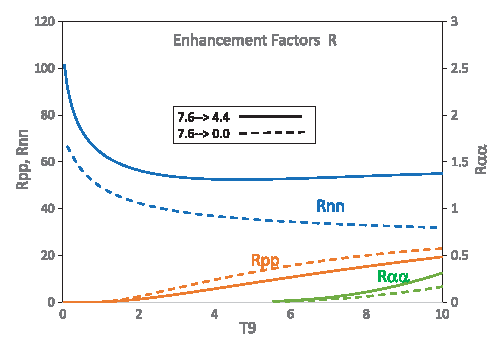
\includegraphics[clip, width=0.6\columnwidth]{R_T.eps}
  \caption[$\gamma$線による脱励起の寿命と粒子散乱による脱励起の寿命の比.]
          {$\gamma$線による脱励起の寿命と粒子散乱による脱励起の寿命の比~\cite{hotdensemedium}.
    Rnn,Rpp,R$\alpha\alpha$はそれぞれ中性子,陽子,$\alpha$粒子と散乱した際の寿命の比を表す.}
  \label{fig::R}
\end{figure}

$\rho\sim\SI{e6}{\gram\per\cubic\centi\metre}$のような高密度環境は宇宙の何処にあるだろうか.
一つの候補として超新星爆発が考えられる.
10--30 $\mathrm{M_{\odot}}$程度の大質量星は,重力崩壊を起こして星の一生を終える.
重力崩壊の際に恒星の中心にある鉄コアの温度が急激に上昇する.
極めて高い温度では高エネルギーの光子によって鉄コアの原子核が陽子や中性子に分解される.
また,密度が非常に高いため式\eqref{eq::neutronize}のように陽子が中性子へ変わる電子捕獲反応が起きる.
\begin{equation}
  {\rm p}+{\rm e}^{-} \rightarrow {\rm n}+\nu_{\rm e}
  \label{eq::neutronize}
\end{equation}
すると,恒星の中心に原始中性子星が形成される.
重力によって中心に降ってくる物質は原始中性子星によって跳ね返され,超新星爆発が起きる.
崩壊前の恒星が持っていた重力エネルギーが熱エネルギーに変換されるので,
原始中性子星の温度は\SI{e10}{\kelvin}に達する.
跳ね返った物質が膨張することで温度が下がっていき,
\SI{7e9}{\kelvin}ほどになると2つの陽子と2つの中性子が融合し$\alpha$粒子が合成される.
このとき,$\alpha$粒子と中性子が高密度かつ高温で存在する環境ができるのである.

\section{測定を行うべき中性子のエネルギー}
式\eqref{eq::R}から分かるように寿命の比$R$を計算するためには,
中性子と${}^{12}\mathrm{C}$の非弾性散乱断面積 [$\sigma_\mathrm{nn'} (E)$] のエネルギー分布が必要となる.
特に,式\eqref{eq::R}から分かるように$R$が$0_2^+$状態の励起エネルギーからのエネルギーに指数関数で依存しているので,
$0_2^+$状態へ励起させることができる中性子エネルギーの閾値付近における断面積が重要となる.
基底状態からの励起を考えると,重心系のエネルギーでは,$E=\SI{7.65}{\mega\electronvolt}$,
${}^{12}\mathrm{C}$の静止系における中性子のエネルギーでは$E_{\text{lab}} = \SI{8.35}{\mega\electronvolt}$である.
%特に,天体中で${}^{12}\mathrm{C}$と散乱した後に中性子が持つエネルギー領域を狙う必要がある.
%Beardら~\cite{hotdensemedium}が考えているような$T\sim\SI{e9}{\kelvin}$では,
%$k_{B}T\sim\SI{100}{\kilo\electronvolt}$である.% 1K = 8.61734e-5 eV
%このような中性子がHoyle状態 (Ex = \SI{7.65}{\mega\electronvolt}) の${}^{12}\mathrm{C}$と散乱すると,
%散乱後の中性子は$E_{\text{n}}\sim\SI{8}{\mega\electronvolt}$となる.
%つまり,式\eqref{eq::tau}に示した脱励起の寿命の計算には
%数 \si{\mega\electronvolt}のエネルギーを持つ中性子と${}^{12}\mathrm{C}$との断面積のエネルギー分布が必要となる.
図\ref{fig::crosssection_pres}~\cite{hotdensemedium}は${}^{12}\mathrm{C}$と中性子(上)または陽子(下)の
各実験室系エネルギーにおける非弾性散乱断面積のエネルギー分布を示す.
点で示される値は測定値,実線で示される値はTALYS による理論計算値を表す.
図\ref{fig::crosssection_pres} (上) から分かるように,
%数 \si{\mega\electronvolt}の領域におけるg.s. $\rightarrow$ Hoyle状態のデータがない.
$E_{\text{lab}} =$ \SIrange{8}{17}{\mega\electronvolt}の領域におけるg.s. $\rightarrow$ Hoyle状態の中性子の測定値がない.
そのため,このエネルギー領域での ${}^{12}\mathrm{C}(\mathrm{n},\mathrm{n}'){}^{12}\mathrm{C} (0_2^+)$ の
断面積の測定が必要となる.
\begin{figure}
  \centering
  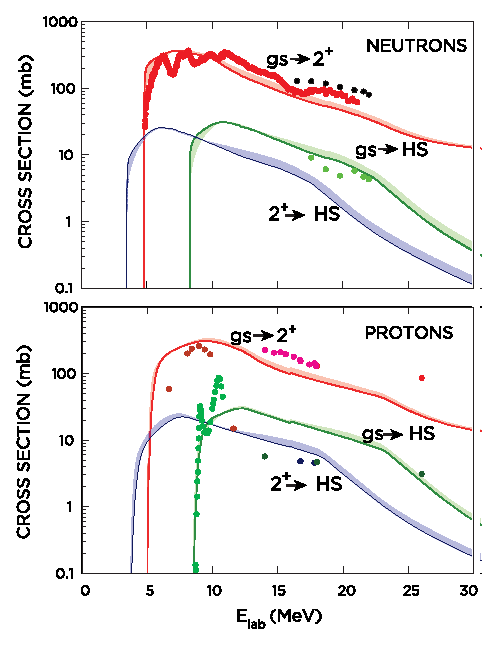
\includegraphics[clip,width=0.6\columnwidth]{cross_section_p_and_n.eps}
  \caption[${}^{12}\mathrm{C}$と中性子 (上段) および陽子 (下段) との非弾性散乱断面積.]
          {${}^{12}\mathrm{C}$と中性子 (上段) および陽子 (下段) との非弾性散乱断面積~\cite{hotdensemedium}.
  実線はTALYS~\cite{talys-1.0} を用いた理論計算,点は測定値を表す.}
  \label{fig::crosssection_pres}
\end{figure}

本研究ではその第一歩として
$E_{\text{n}} = \SI{14}{\mega\electronvolt}$の中性子を用いて断面積の測定を行い,
${}^{12}\mathrm{C}(\mathrm{n},\mathrm{n}'){}^{12}\mathrm{C} (0_2^+)$反応の断面積測定の実現可能性を確認する.
\SI{14}{\mega\electronvolt}は式\eqref{eq::dt}に示すデューテリウムとトリチウムの反応(DT 反応)を
用いて生成可能なエネルギーである.
この反応は2体反応であるため,放出角度により中性子のエネルギーが一意に決まる.%単色エネルギーの中性子となる.
\begin{equation}
  \mathrm{d} + \mathrm{t} \rightarrow \alpha\ (\SI{3.5}{\mega\electronvolt}) + \mathrm{n}\ (\SI{14}{\mega\electronvolt})
  \label{eq::dt}
\end{equation}
単色エネルギーの中性子を用いることで,中性子のエネルギー測定を行う必要が無くなる.
%核破砕で生成される
%このDT 反応で生成される$14~{\rm MeV}$の中性子と炭素との反応は核融合炉の開発で重要である.
ITER~\cite{iter}などの核融合炉ではこのDT 反応を用いて質量エネルギーを取り出す.
核融合炉の中で生成される\SI{14}{\mega\electronvolt}の中性子は構造材の原子核と反応し損傷させるため,
構造材の中に多く含まれる炭素との反応が詳しく調べられている~\cite{takahashietal,kondoetal}.
${}^{12}\mathrm{C}(\mathrm{n},\mathrm{n}'+3\alpha)$反応の全断面積は\SI{209}{\milli\barn},
分岐比は表\ref{tab::branchingratio}の通りである.
また,微分断面積の角度分布を図\ref{fig::sig_angle_dist}に示す.
これらの測定値と本研究での測定値を比較することによって測定方法の妥当性を確認することが可能となる.
単色エネルギーの中性子を生成可能であること,他データと測定結果の比較が可能であることの2点より,
測定方法の検証として\SI{14}{\mega\electronvolt}の中性子ビームを用いて
${}^{12}\mathrm{C}(\mathrm{n},\mathrm{n}'){}^{12}\mathrm{C}(0_2^+)$反応の断面積の測定を行う.

\begin{table}
  \centering
  \caption[${}^{12}\mathrm{C}(\mathrm{n},\mathrm{n}'+3\alpha)$反応のチャンネルとその分岐比.]
          {${}^{12}\mathrm{C}(\mathrm{n},\mathrm{n}'+3\alpha)$反応のチャンネルとその分岐比~\cite{kondoetal}.
            ${}^{12}\mathrm{C}$の励起状態から$3\alpha$に,${}^{9}\mathrm{Be}$の励起状態から$2\alpha$に崩壊する.}
  \label{tab::branchingratio}
  \begin{tabular}{lc}
    \toprule
    \multicolumn{1}{c}{Reaction channel} & Branching ratio (\%)\\
    \midrule
    ${}^{12}\mathrm{C}(\mathrm{n},\mathrm{n}'){}^{12}\mathrm{C}^{*}$(\SI{7.65}{\mega\electronvolt}) & 4\\
    ${}^{12}\mathrm{C}(\mathrm{n},\mathrm{n}'){}^{12}\mathrm{C}^{*}$(\SI{9.64}{\mega\electronvolt}) & 33\\
    ${}^{12}\mathrm{C}(\mathrm{n},\mathrm{n}'){}^{12}\mathrm{C}^{*}$(\SI{10.3}{\mega\electronvolt}) & 16\\
    ${}^{12}\mathrm{C}(\mathrm{n},\mathrm{n}'){}^{12}\mathrm{C}^{*}$(\SI{10.84}{\mega\electronvolt}) & 6\\
    ${}^{12}\mathrm{C}(\mathrm{n},\mathrm{n}'){}^{12}\mathrm{C}^{*}$(\SI{11.83}{\mega\electronvolt}) & 4\\
    ${}^{12}\mathrm{C}(\mathrm{n},\alpha){}^{9}\mathrm{Be}^{*}$(\SIrange{1.68}{3.05}{\mega\electronvolt}) & 24\\
    ${}^{12}\mathrm{C}(\mathrm{n},\alpha){}^{9}\mathrm{Be}^{*}$(\SI{4.7}{\mega\electronvolt}) & 13\\
    \bottomrule
  \end{tabular}
\end{table}

\begin{figure}
  \centering
  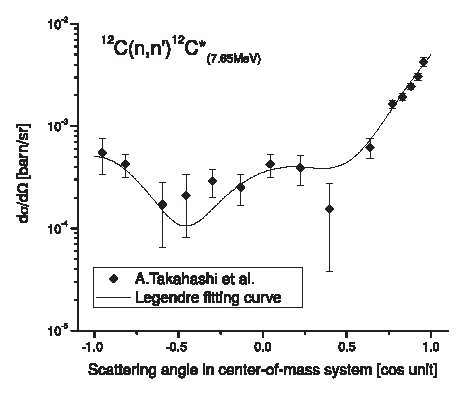
\includegraphics[clip, width=0.6\columnwidth]{cross_section_12C_n_n_12C_7.65.eps}
  \caption[${}^{12}\mathrm{C}(\mathrm{n},\mathrm{n}'){}^{12}\mathrm{C} (0_2^+)$の微分断面積の角度分布.]
          {${}^{12}\mathrm{C}(\mathrm{n},\mathrm{n}'){}^{12}\mathrm{C} (0_2^+)$の微分断面積の角度分布~\cite{kondoetal}.}
  \label{fig::sig_angle_dist}
\end{figure}

\section{測定に用いる実験装置}
\label{seq::detector_using_experiment}
${}^{12}{\rm C} (0_2^+)$から崩壊して生成した3つの$\alpha$粒子を測定することで,断面積を決定する.
図\ref{fig::sig_angle_dist}の微分断面積で散乱し,
励起した${}^{12}\mathrm{C}(0_2^+)$から$\alpha$粒子が等方的に崩壊すると仮定すると,
${}^{12}\mathrm{C} (0_2^+)$から放出された$\alpha$粒子は
図\ref{fig::alpha_E_En_dep_w_l}に示すエネルギーの分布を持つ.
ここでは,エネルギーによらずに同じ微分断面積を仮定した.
横軸は入射中性子のエネルギー,縦軸は崩壊後の$\alpha$粒子のエネルギーである.
図\ref{fig::alpha_E_En_dep_w_l}から中性子のエネルギーに関わらず
$\alpha$粒子のエネルギーは約\SI{0.1}{\mega\electronvolt}が最頻値となっていることが分かる.
\SI{1}{\mega\electronvolt}より大きい領域は重心運動と同じ方向に放出された$\alpha$粒子が
ブーストされエネルギーが大きくなったものと考えられる.
一方,重心運動と異なる方向に放出された$\alpha$粒子は,
あまりブーストされずに典型的には励起エネルギーと3$\alpha$崩壊閾値の差分を3等分したエネルギー
($\SI{0.38}{\mega\electronvolt}\div 3 \sim \SI{0.1}{\mega\electronvolt}$) を持つ.
図\ref{fig::sig_angle_dist}から分かるように
${}^{12}\mathrm{C}(\mathrm{n},\mathrm{n}'){}^{12}\mathrm{C}(0_2^+)$反応では前方散乱の断面積が大きく,
${}^{12}\mathrm{C} (0_2^+)$が重心運動方向と異なる方向に散乱される確率が高い.
そのため,$\alpha$粒子はあまり重心運動によってブーストされる効果を受けずに,
中性子のエネルギーに関わらず\SI{0.1}{\mega\electronvolt}付近で最大となる.
図\ref{fig::alpha_E_dist}は中性子のエネルギーが\SI{14}{\mega\electronvolt}のときの分布である.
図\ref{fig::alpha_E_dist}の塗りつぶし部分は最大値を中心に全体の8割となる領域を示しており,
\SIrange{0}{0.6}{\mega\electronvolt}の範囲である.
このような低エネルギーの$\alpha$粒子を効率よく検出するためには,
標的中で$\alpha$粒子が停止しないようにしなければならない.
例えば,\SI{500}{\kilo\electronvolt}の$\alpha$粒子ではおよそ\SI{350}{\micro\gram\per\square\centi\metre}の
炭素箔標的で停止してしまう.
更に低いエネルギーの$\alpha$粒子も検出しようとすると,更に標的を薄くしなければならない.
このような低エネルギー粒子の測定には,検出器そのものが標的となるアクティブ標的が有効である.

図\ref{fig::alpha_theta_En_dep}は$\alpha$粒子の実験室系での角度分布である.
横軸は入射中性子のエネルギー,縦軸は$\alpha$粒子の入射中性子の運動方向に対する角度を表す.
$\alpha$粒子のエネルギー分布と同様に入射中性子のエネルギーにあまり依存していない.
図\ref{fig::alpha_theta_dist}は入射中性子が\SI{14}{\mega\electronvolt}のときの角度分布である.
図\ref{fig::alpha_theta_dist}の塗りつぶしは最大値を中心に全体の8割となる領域を示しており,
\SIrange{7.5}{75.1}{\degree} である.
%この図からもわかるように広い角度領域に$\alpha$粒子は崩壊する.
このような広い角度に放出される3つの$\alpha$粒子すべてを効率的に検出するためには大立体角を覆う検出器が必要となる.

このような要求を満たす検出器として検出ガスを散乱標的として用いるtime projection chamber (TPC) が有効である.
TPC は荷電粒子のトラックを検出することができるガス検出器であり,
ALICE 実験~\cite{alice-tpc}やLEPS2~\cite{kobayakawa_thesis}などで広く用いられている.
アクティブ標的TPC を用いることで,低エネルギー荷電粒子を大立体角で検出することが可能となる.
近年,不安定核実験のためにMAYA~\cite{maya}やCAT~\cite{cat-tpc},AT-TPC~\cite{at-tpc}など
アクティブ標的を用いたTPC が開発されている~\cite{active-tpc}.
その1つとして我々が開発したMAIKo ($\mu$-PIC based active target for inverse kinematics $_{\circ}$)
 TPC~\cite{maiko, mupic}がある.
近年,RCNP でMAIKo TPC を用いて低エネルギー$\alpha$粒子を測定する実験~\cite{Furuno2019}が行われた.
MAIKo TPC を用いることで低エネルギーの$\alpha$粒子を大立体角で検出することができる.
本研究ではMAIKo TPC を用いて${}^{12}\mathrm{C}(\mathrm{n},\mathrm{n}'){}^{12}\mathrm{C} (0_2^+)$反応を測定することを目指す.
\begin{figure}
  \centering
  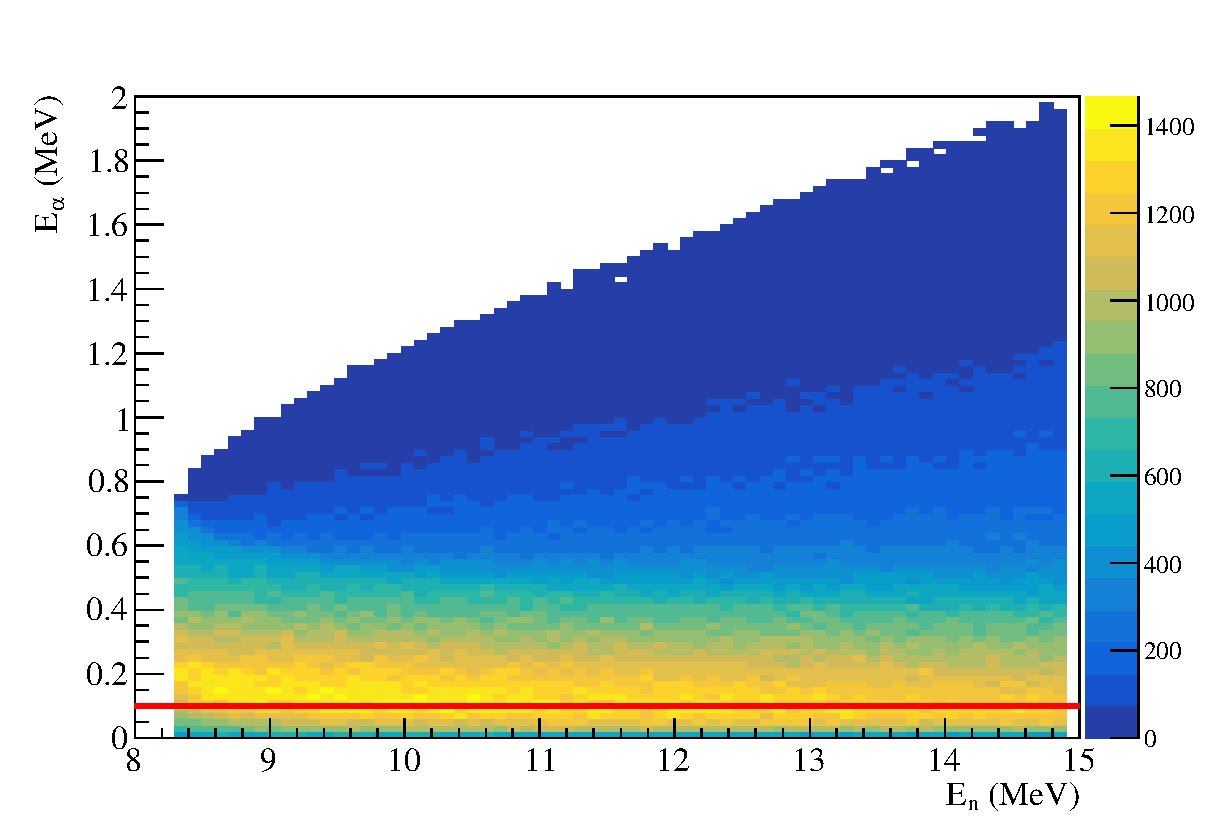
\includegraphics[clip, width=0.8\columnwidth]{alpha_E_En_dep_w_l.eps}
  \caption{${}^{12}\mathrm{C} (0_2^+)$から放出された$\alpha$粒子のエネルギー分布.
    横軸は入射中性子のエネルギー,縦軸は崩壊後の$\alpha$粒子のエネルギーである.
    赤い実線は$E_{\alpha}$ = \SI{0.1}{\mega\electronvolt}を表す.}
  \label{fig::alpha_E_En_dep_w_l}
\end{figure}
\begin{figure}
  \centering
  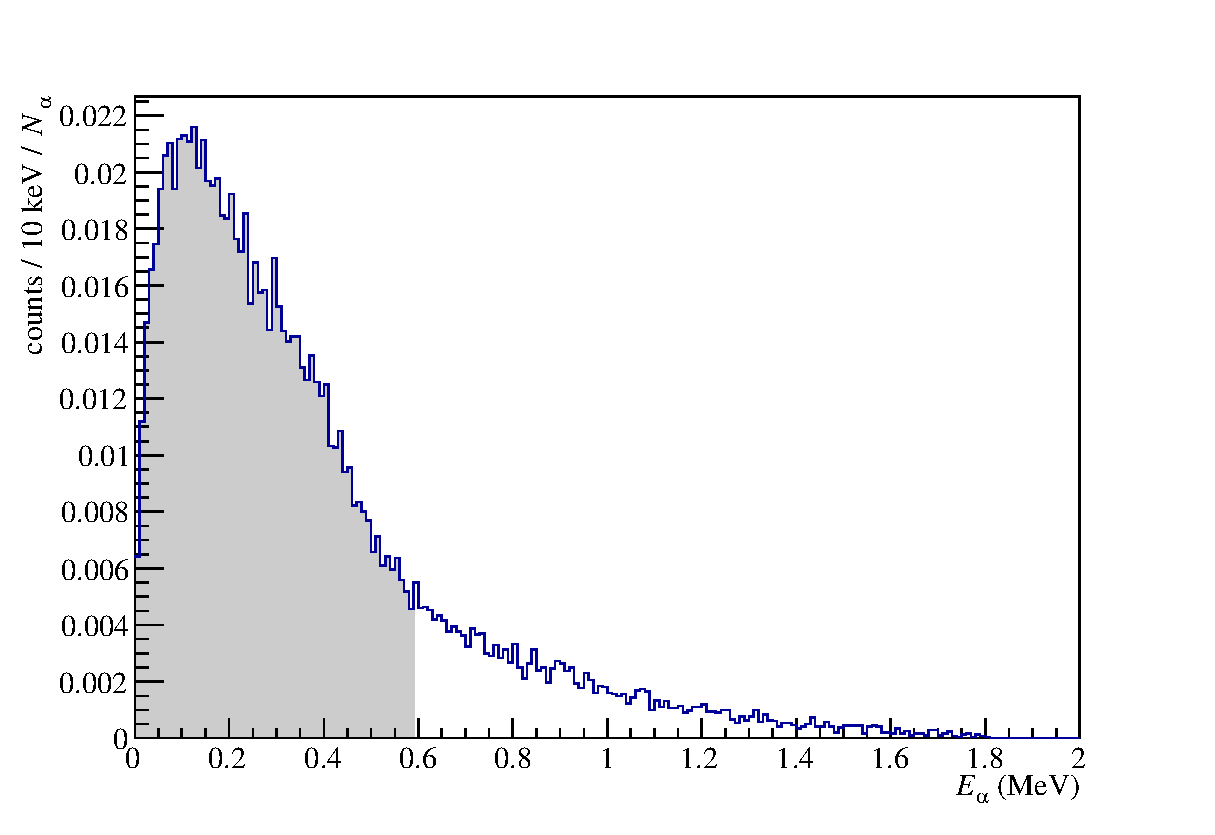
\includegraphics[clip, width=0.8\columnwidth]{alpha_e_dist_sim_region.eps}
  \caption[${}^{12}{\rm C} (0_2^+)$から放出された$\alpha$粒子のエネルギー分布.]
          {$E_{\mathrm{n}}=\SI{14}{\mega\electronvolt}$のときの,
            ${}^{12}{\rm C} (0_2^+)$から放出された$\alpha$粒子のエネルギー分布.
            ${}^{12}\mathrm{C}$から放出される3つの$\alpha$粒子すべての分布を表している.}
          \label{fig::alpha_E_dist}
\end{figure}
\begin{figure}
  \centering
  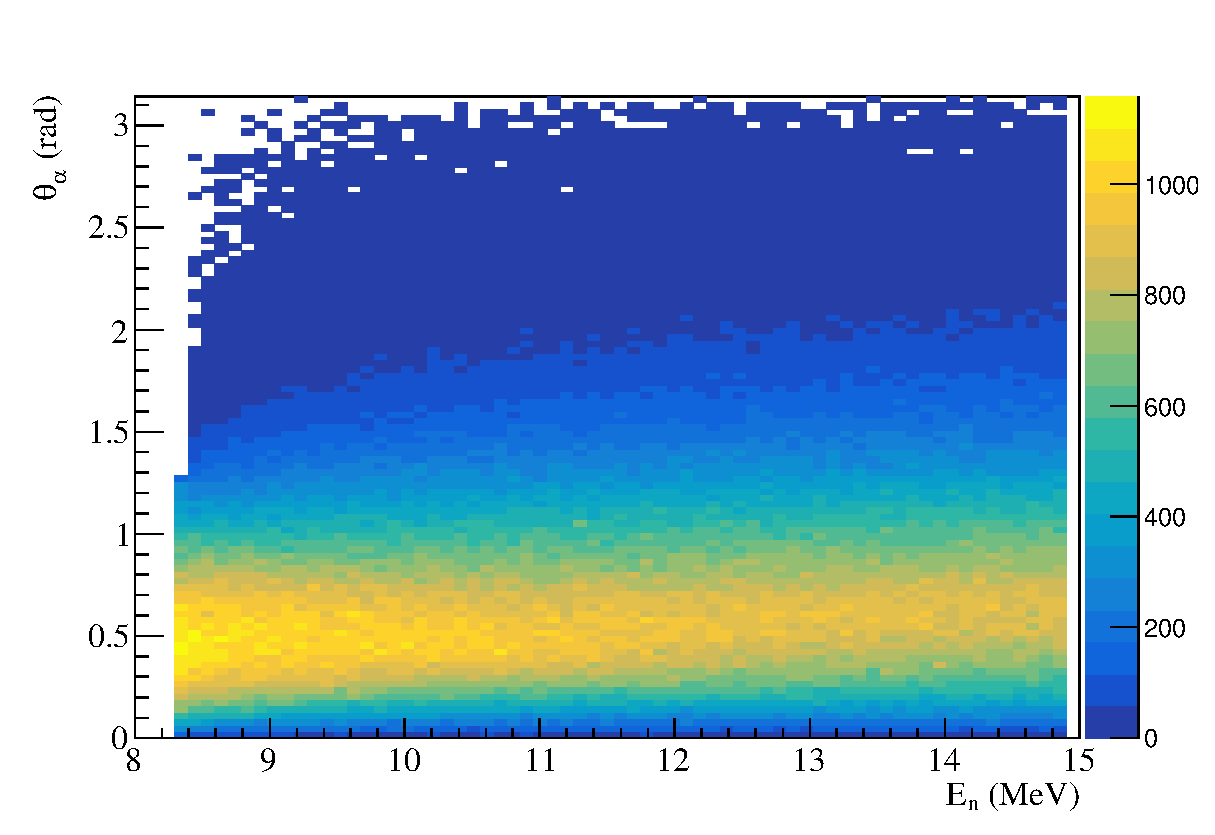
\includegraphics[clip, width=0.8\columnwidth]{alpha_theta_En_dep.eps}
  \caption{${}^{12}{\rm C} (0_2^+)$から放出された$\alpha$粒子の角度分布.}
  \label{fig::alpha_theta_En_dep}
\end{figure}
\begin{figure}
  \centering
  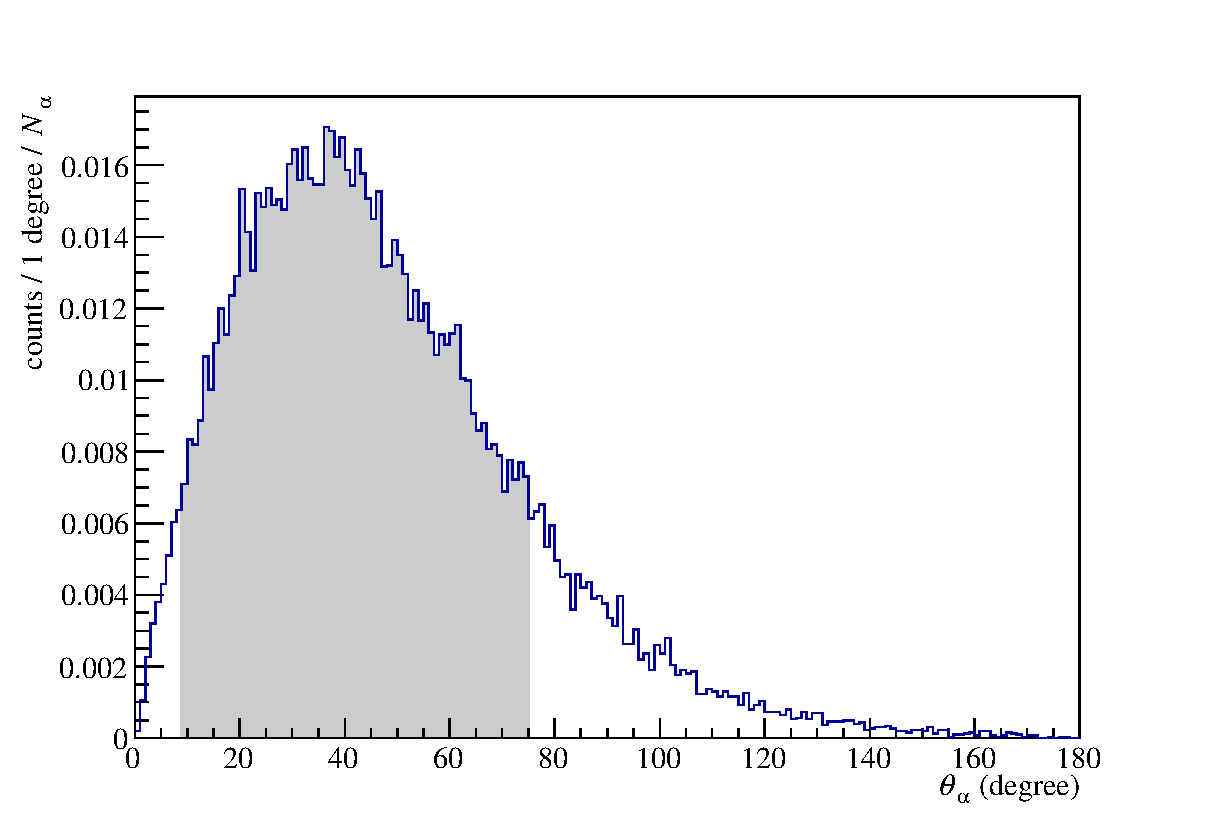
\includegraphics[clip, width=0.8\columnwidth]{alpha_theta_dist_region.eps}
  \caption[${}^{12}{\rm C} (0_2^+)$から放出された$\alpha$粒子の角度分布.]
          {$E_{\mathrm{n}}=\SI{14}{\mega\electronvolt}$のときの,
            ${}^{12}{\rm C} (0_2^+)$から放出された$\alpha$粒子の角度分布.
            ${}^{12}\mathrm{C}$から放出される3つの$\alpha$粒子すべての分布を表している.
          }
  \label{fig::alpha_theta_dist}
\end{figure}
%ピーク周りに8割を取ってくると0.13 rad -- 1.31 rad, 0 -- 0.595 MeV

%また,TPC は荷電粒子のトラックを検出することができる検出器である.
%荷電粒子を入射粒子として用いる実験では,標的粒子と散乱しなかった入射粒子のトラックも検出する.
%このような事象は背景事象となる.
%本研究では中性子を入射するため,そのような背景事象は発生しない.
%そのため,高強度の中性子ビームを用いた実験が可能であり,
%散乱事象を効率的に検出することができる.

\section{本研究の目的}
${}^{12}\mathrm{C}(\mathrm{n},\mathrm{n}'){}^{12}\mathrm{C} (0_2^+)$反応の断面積測定は,
低エネルギーの$\alpha$粒子を検出する必要がある.
\ref{seq::detector_using_experiment}節で述べたように,
MAIKo TPC を用いれば効率的に3つの低エネルギー$\alpha$粒子を検出することが可能となる.
しかし,崩壊してできた$\alpha$粒子が持つ運動エネルギーは広がりを持ち,数十倍違うこともある.
そのため,より効率的に全ての粒子を測定するための条件を検討する必要がある.
MAIKo TPC では使用する検出ガスの種類,圧力,電圧等の多くのパラメータを調整することができる.
本研究では効率的に$\alpha$粒子を検出することができる検出ガスの候補を複数選出し,
$\alpha$線源を用いて性能試験を行う.
それらのガスについて中性子との散乱で${}^{12}\mathrm{C}$原子核が3つの$\alpha$粒子に崩壊するイベントをシミュレートし,
MAIKo TPC から得られるであろう画像を生成する.
シミュレーションで生成した画像に対して解析を行い,検出効率,エネルギー分解能,角度分解能を評価する.
評価結果から実験で用いる検出ガスを決定する.
また,正しく解析を行える割合やこの測定方法で期待される収量の評価を行い,実験の実現可能性を検討する.
\end{document}

\documentclass[../master]{subfiles}

\begin{document}

\chapter{MAIKo TPC}
\section{MAIKo TPC とは}
TPC は荷電粒子のトラックを検出するために広く用いられているガス検出器である.
図\ref{fig::MAIKo_view}にTPC の模式図を示す.
荷電粒子がTPC の検出ガス中を通過するとき,トラックの周囲の粒子をイオン化させる.
イオン化で発生した電子をドリフト電場 (図\ref{fig::MAIKo_view}中$y$軸方向) により
読み出し面にドリフトさせることでトラックを検出する.
電子が読み出し面に到達する時間差によって,$y$軸方向の位置を決定することができる.
読み出し面によって$x, z$座標を決定することで,3次元的にトラックを決定できる.

TPC の有感領域中で入射粒子と標的粒子が反応することで,
散乱点の周りを有感領域で覆うことができるため,
散乱で放出される低エネルギーの荷電粒子を大立体角で検出することが可能となる.
図\ref{fig::MAIKo_view}は検出器中で中性子と${}^{12}\mathrm{C}$との散乱によって,
3つの$\alpha$粒子が放出されたイベント表す.
これを実現する方法として,検出器そのものを標的として用いるアクティブ標的がある.
アクティブ標的を用いたTPC としてMAIKo TPC が開発された.
MAIKo TPC は検出ガスを封入するチェンバー (MAIKo チェンバー) と
ドリフト電場を形成するケージ (ドリフトケージ) とからなる.
ドリフトケージを図\ref{pic::MAIKo_cage}に示す.
MAIKo チェンバーを図\ref{pic::MAIKo_chamber}に示す.
ドリフトケージをMAIKo チェンバー内に設置して用いる.
\begin{figure}
  \centering
  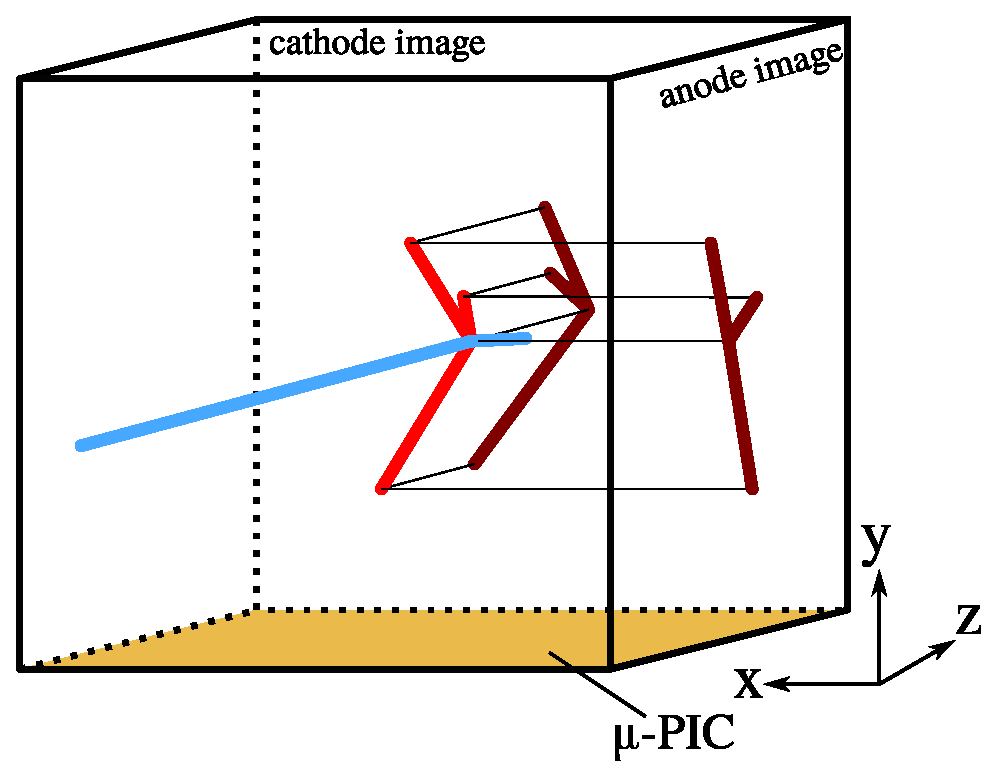
\includegraphics[clip, width=0.7\columnwidth]{MAIKo2.eps}
  \caption[MAIKo TPC の概観図.]{MAIKo TPC の概観図.
    図では紙面手前から入射した中性子 (青) がTPC の中の${}^{12}{\rm C}$と
    散乱して3つの$\alpha$粒子 (赤) に崩壊した事象を表す.
    anode image ($zy$平面) と cathode image ($zy$平面) の2平面に荷電粒子のトラックが射影される.
    中性子は電荷を持たないためanode \& cathode image にトラックとして検出されない.
  }
  \label{fig::MAIKo_view}
\end{figure}
\begin{figure}
  \centering
  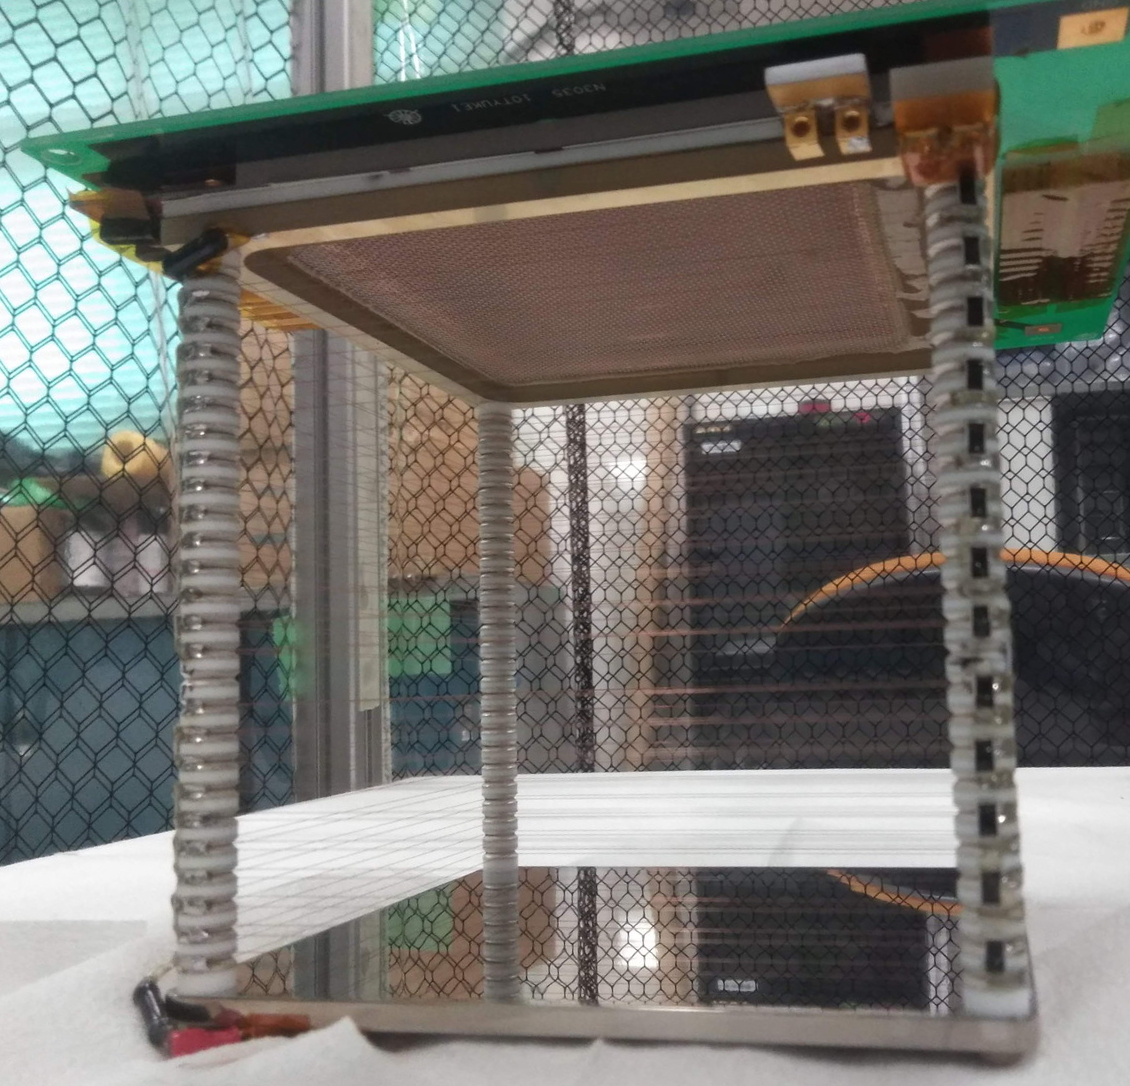
\includegraphics[clip, width=0.7\columnwidth]{IMG_20190731_110230_clpd.jpg}
  \caption[ドリフトケージの概観.]
          {ドリフトケージの概観.
          図\ref{fig::MAIKo_view}の模式図とはドリフト方向が上下が反転している.}
  \label{pic::MAIKo_cage}
\end{figure}
\begin{figure}
  \centering
  \begin{subfigure}{0.45\columnwidth}
    \centering
    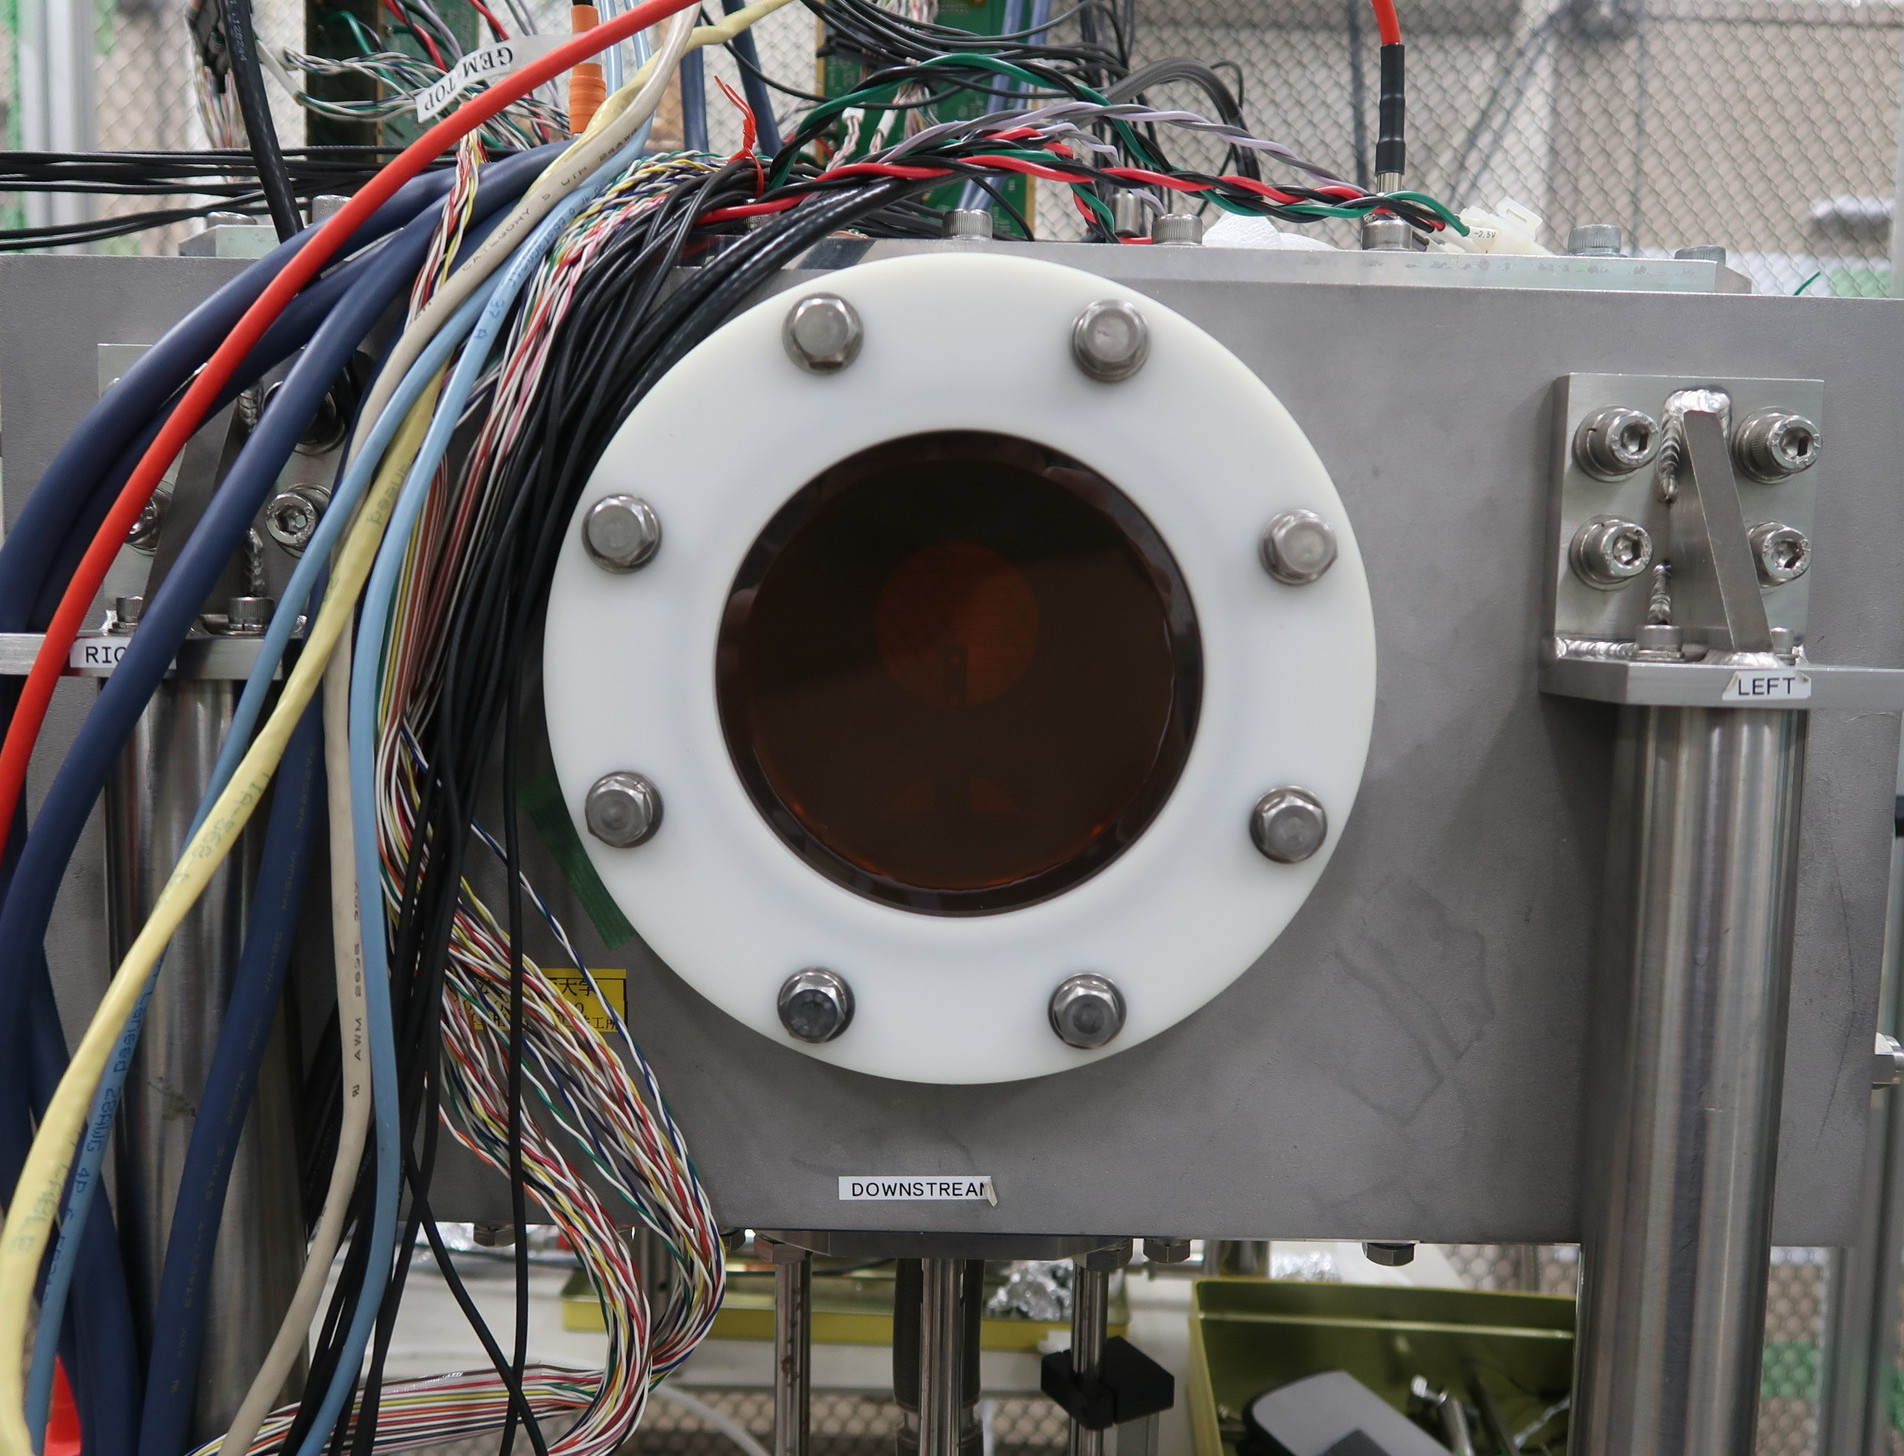
\includegraphics[clip, width=\columnwidth]{IMG_2925_clpd.jpg}
    \caption{外側.}
    \label{pic::MAIKo_chamber_out}
  \end{subfigure}
  \begin{subfigure}{0.45\columnwidth}
    \centering
    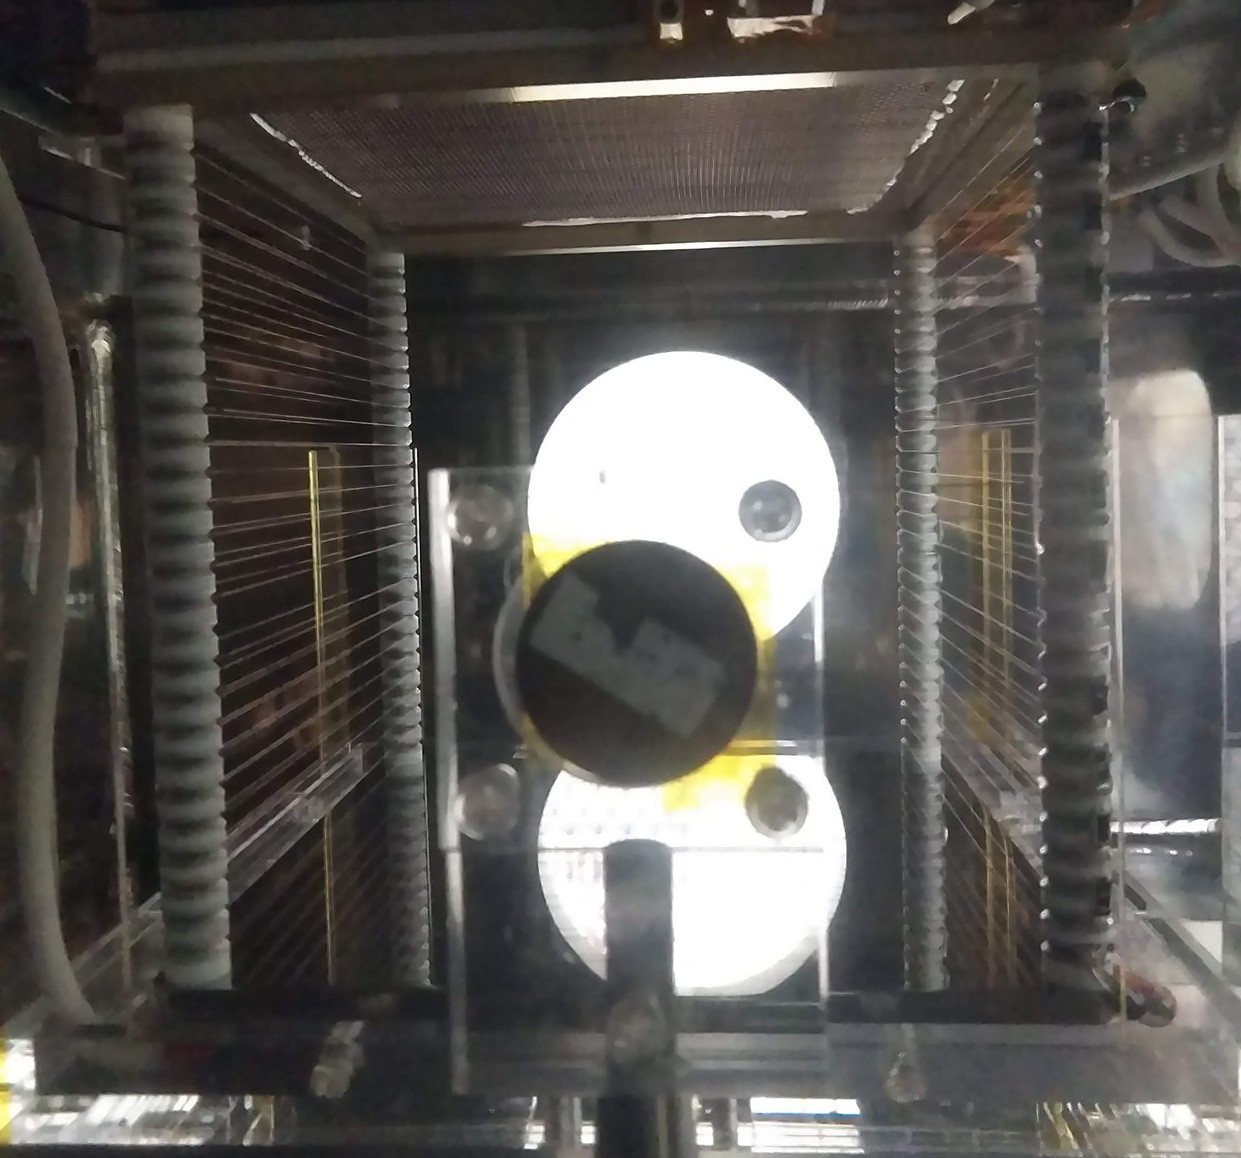
\includegraphics[clip, width=\columnwidth]{IMG_20190801_160046_clpd.jpg}
    \caption{内側.}
    \label{pic::MAIKo_chamber_in}
  \end{subfigure}
  \caption{MAIKo チェンバー.}
  \label{pic::MAIKo_chamber}
\end{figure}

図\ref{fig::MAIKo_cage}にドリフトケージの模式図を示す.
ドリフトケージはplate,wire,grid,GEM (gas electron multiplier),$\mu$-PICからなる.
plate,grid,GEM,$\mu$-PICにHV が接続されている.
plate,wire,girdの間は\SI{10}{\mega\ohm}の抵抗で繋がれている.
GEM とHV は\SI{1}{\mega\ohm}と\SI{20}{\mega\ohm}の抵抗で繋がれている.
plateからgridの間の領域をドリフト領域,
gridから$\mu$-PICの間の領域を増幅領域,
$\mu$-PICの周囲を読み出し領域と呼ぶ.
\begin{figure}
  \centering
  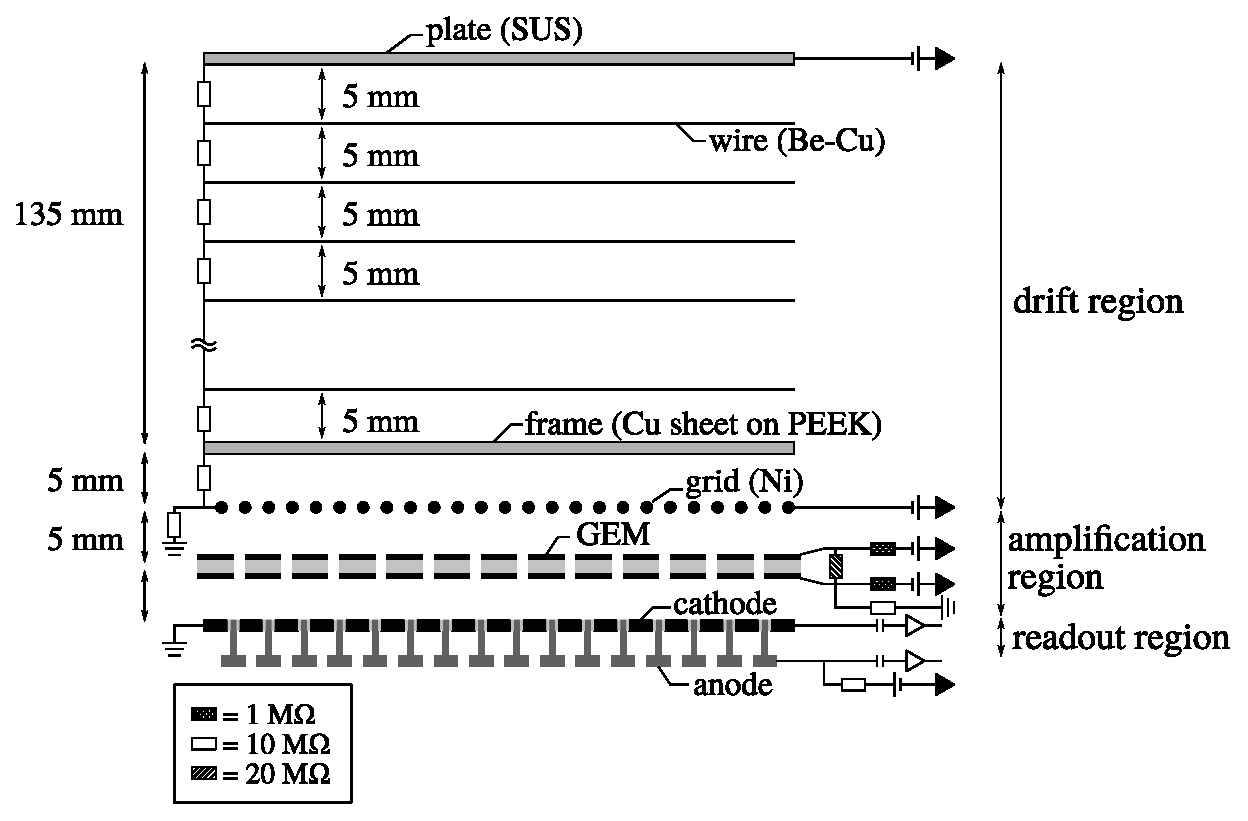
\includegraphics[clip, width=\columnwidth]{MAIKo_cage.eps}
  \caption{ドリフトケージの構造.}
  \label{fig::MAIKo_cage}
\end{figure}

%plate とgrid に電圧をかけることでドリフト領域にドリフト電場を形成する.
%ドリフト領域を荷電粒子が通過する際に生成された電子がドリフト電場によって増幅領域へ移動する.
%ドリフト電場を一様に形成するために5 mm間隔でドリフト領域の周囲にwire を巻いてある.
%ドリフト領域はドリフト方向に140 mm である.
%ドリフトしてきた電子は,まずGEM (gas electron multiplier) で増幅される.
%増幅した電子およびイオンによって$\mu$-PIC のanode とcathode に誘起された信号を読み出す.
%$\mu$-PIC では信号の読み出しだけでなく電子の増幅も行われる.

\subsection{ドリフト領域}
grid からplate の方向 (図\ref{fig::MAIKo_cage}では上向き) にドリフト電場を作ることで
トラックの周りに発生した電子を増幅領域へドリフトさせる.
plateとgridにそれぞれ高電圧を印加することでドリフト電場を形成する.
ドリフト電場の一様性が高いほど,電子を均等にドリフトすることができる.
ドリフト電場を一様に形成するために\SI{10}{\mega\ohm}の抵抗で接続されたwire が
\SI{5}{\milli\metre}間隔で巻かれている~\cite{furuno}.
ドリフト領域はドリフト電場の方向に\SI{140}{\milli\metre}である.
ドリフト領域がMAIKo TPC の有感領域となる.

\subsection{増幅領域}
MAIKo TPC ではGEM と$\mu$-PICを用いて電子の増幅を行う.
GEM は,図\ref{pic::GEM}のようにポリマーのフィルムの表面を銅で被覆し,
直径\SI{70}{\micro\metre} の穴を\SI{140}{\micro\metre}間隔で\SI{1}{\square\milli\metre}あたり
100 個の密度で開けたものである.
銅の2つの層はポリマーによって絶縁されている.
銅の両面に電圧を印加することによって,穴の中に高電場が形成されドリフトしてきた電子が増幅される.
\begin{figure}
  \centering
  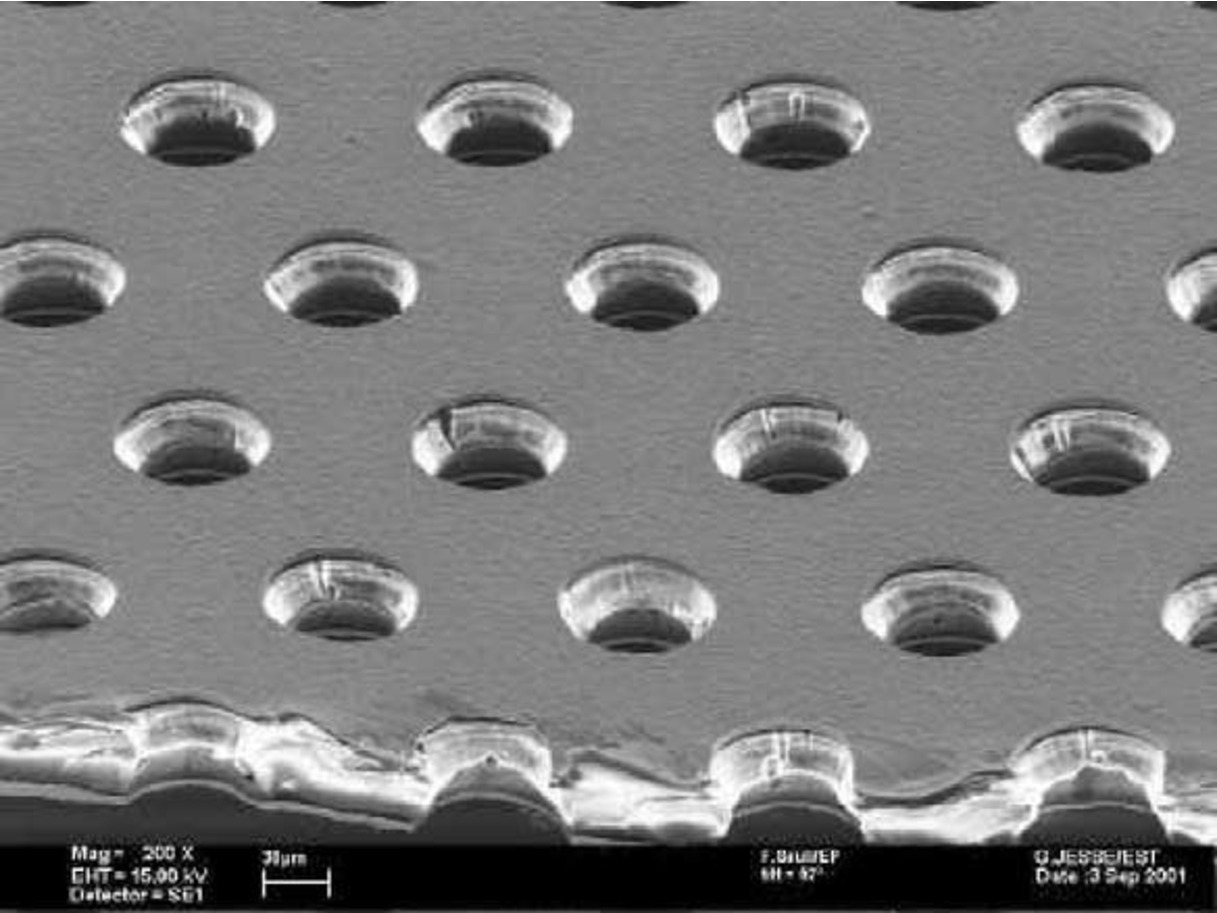
\includegraphics[clip, width=0.7\columnwidth]{gem_structure.pdf}
  \caption{GEM の拡大図~\cite{gem_compass}.}
  \label{pic::GEM}  
\end{figure}

$\mu$-PIC は図\ref{fig::mupic}のようにanode strip とcathode strip が直交するように配置されている.
anode strip,cathode strip ともに\SI{400}{\micro\metre}間隔でそれぞれ256~ch分割されている.
直径\SI{50}{\micro\metre}の円柱状のanode 電極に高電圧をかけることで高電場を形成することができ,
$\mu$-PICによって信号が読み出される直前に電子が増幅される.
\begin{figure}
  \centering
  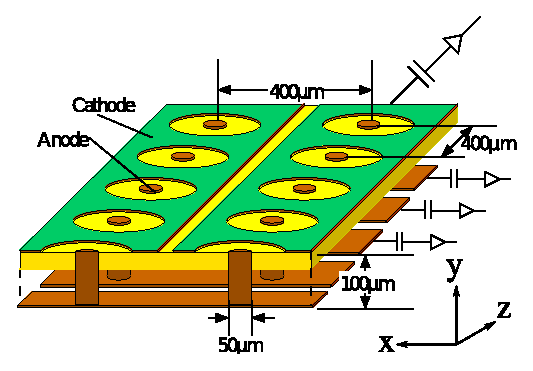
\includegraphics[clip, width=0.7\columnwidth]{upic_struc_xyz.eps}
  \caption[$\mu$-PICの概観図.]{$\mu$-PICの概観図.
    図中の横方向にanode strip,奥行き方向にcathode strip が配置されている.
  }
  \label{fig::mupic}
\end{figure}

\subsection{読み出し領域}
\label{sec::mu-pic}
図\ref{fig::MAIKo_view}中でanode strip は$x$軸,cathode strip は$z$軸と平行になるように$\mu$-PICが配置されている.
GEMと$\mu$-PICにより増幅された電子をanode strip とcathode strip により読み出し,
それぞれ$z$座標,$x$座標を検出することができる.
また,anode strip とcathode strip で検出される信号の時間分布により$y$軸座標を決定することができる.

MAIKo TPC からは図\ref{fig::MAIKo_view}のようにトラックが
anode strip に垂直な面 ($z-y$平面) に射影されたanode image と
cathode strip に垂直な面 ($x-y$平面) に射影されたcathode image の2つの画像が出力される.
MAIKo TPC から得られる画像の1例を図\ref{fig::track_demo}に示す.
anode strip とcathode strip はそれぞれ256~chで構成され,
読み出される信号は\SI{100}{\mega\hertz}で1,024~samples測定し,
閾値に対するtime over threshold (TOT) を取得する.
TOT は閾値以上を1,以下を0としたものである.
出力されるデータは解像度が$256\times1,014$~pixels の白黒画像となる.
また,anode strip,cathode strip ともに32~chごとにまとめて信号を波形としてFADC で取得している.
32~chごとにまとめられるため,anode strip,cathode strip ともに8~chずつFADC でデータを取得している.
FADC で取得した信号の一例を図\ref{fig::FADC_waveform}に示す.
FADC は\SI{25}{\mega\hertz}で波形を取得する.
\begin{figure}
  \centering
  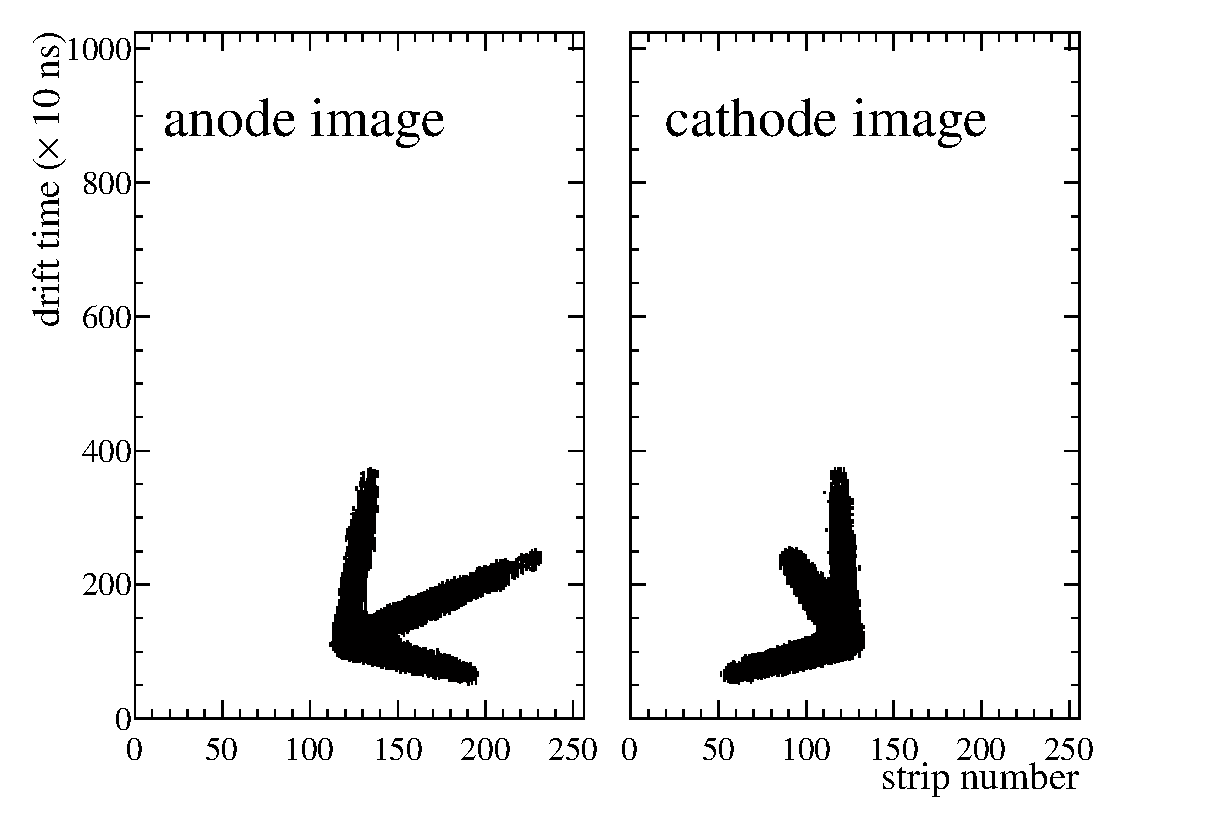
\includegraphics[clip, width=0.9\columnwidth]{10024_4.eps}
  \caption[MAIKo TPC から得られる画像データの一例.]
          {MAIKo TPC から得られる画像データの一例.
          このイベントは\ref{chap::simulation}章で述べるシミュレーションによって生成したデータである.}
  \label{fig::track_demo}
\end{figure}
\begin{figure}
  \centering
  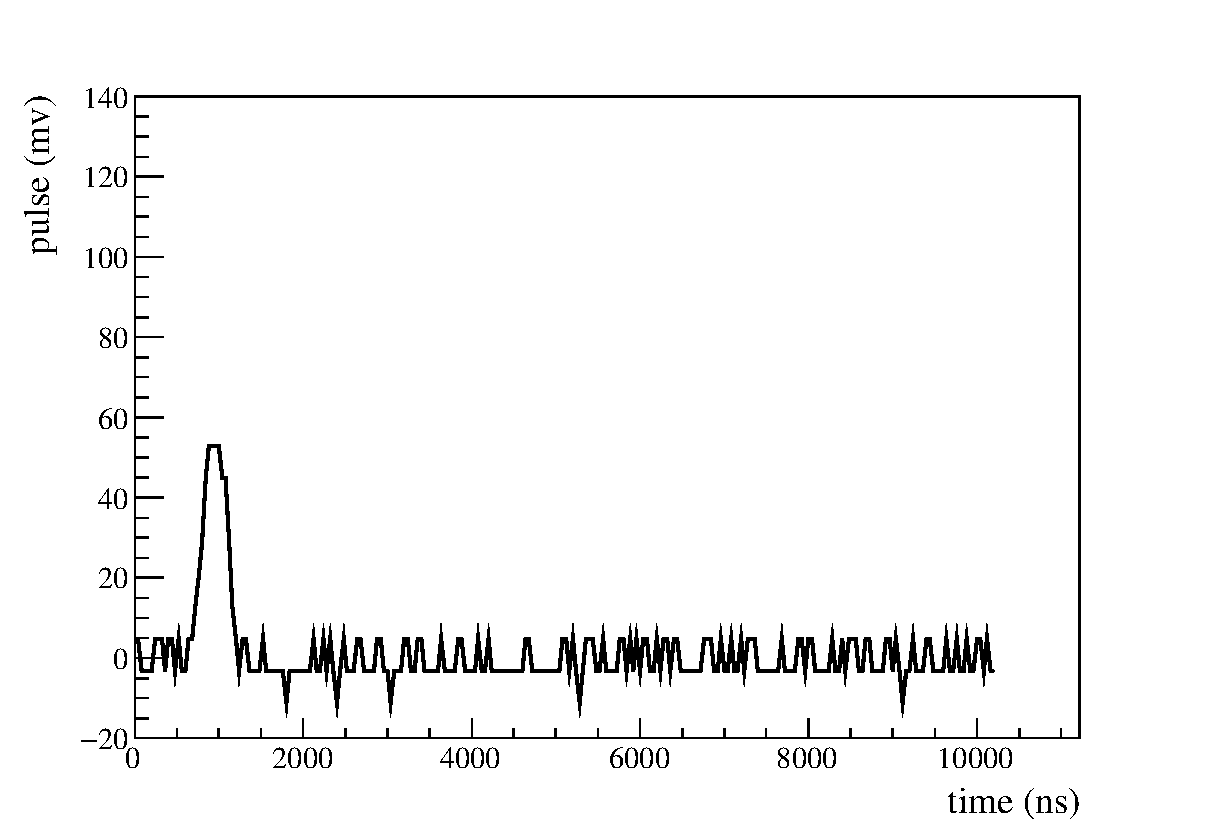
\includegraphics[clip, width=0.7\columnwidth]{0210_waveform_2.eps}
  \caption[FADCで取得された$\mu$-PICの波形の一例.]
          {FADCで取得された$\mu$-PICの波形の一例.
          この波形は\isoButaneHydro を検出ガスとして求めた際のものである.}
  \label{fig::FADC_waveform}
\end{figure}

\section{検出ガスの候補}
\label{sec::detection_gas_candidate}
標的に${}^{12}{\rm C}$を用いるため,分子中に炭素を含むガスを検出ガスに用いる必要がある.
${}^{12}{\rm C}$以外の原子核が含まれると背景事象となる.
陽子,${}^{4}{\rm He}$と14 MeV の中性子の散乱は複数の荷電粒子に崩壊しないため,
トラックの本数から背景事象を取り除くことができる.
そこで,水素と炭素以外の原子が含まれない炭化水素を検出ガスに用いる.
代表的な炭化水素に,メタン (\Methane) やエタン (${\rm C_{2}H_{6}}$),
イソブタン (\isoButane) がある.
また,水素ガスやヘリウムガスとの混合ガスも用いることができる.
検出ガスとして求められる性能には以下のようなものがある.
\begin{itemize}
\item
  放電しにくい.(安定なTPC の運用)
\item
  $\alpha$粒子のエネルギー損失 ($dE/dx$) が適切である.(トラックを正しく抽出)
\item
  適切なドリフト速度を達成できる.(有感領域を効率的に使用)
\item
  適切なドリフト電場のもとでディフュージョンが小さい.(複数のトラックを正しく抽出)
\item
  ${}^{12}{\rm C}$の量が少なくない.(散乱標的の量)
\end{itemize}
これらの項目を基準に検出ガスの種類と圧力の決定を行う.

\subsection{$\alpha$粒子のエネルギー損失}
MAIKo TPC では荷電粒子のエネルギーと運動量をトラックの長さと方向から決定するため,
トラックを正しく抽出することが必要となる.
荷電粒子のエネルギー損失 ($dE/dx$) が大きくなりすぎると検出ガス中での飛行距離が短くなり,
トラックとして識別することが難しくなる.
また,$dE/dx$ が小さくなりすぎるとトラックが有感領域で止まらず,
トラックの長さを決定することができなくなる.
検出する対象である$\alpha$粒子の $dE/dx$ が適切な大きさとなるガスの種類と圧力の候補を選出する.

まず,代表的な炭化水素である\Methane を考える.
ガス中で\SI{10}{\milli\metre} 以上飛行し,MAIKo TPC の有感領域中で停止する$\alpha$粒子を検出可能な$\alpha$粒子とする.
全ての$\alpha$粒子を検出できたイベントの割合を検出率とする.
図\ref{fig::alpha_E_dist}に示したエネルギー分布の$\alpha$粒子のうち,
検出率の圧力依存性を図\ref{fig::efficiency_P_dist}に示す.
このとき,散乱点がビーム軸上に一様に分布していると仮定した.
図\ref{fig::efficiency_P_dist}から分かるように,\SI{50}{\hecto\pascal} で最大となっている.
\SI{50}{\hecto\pascal}のときの\Methane の$dE/dx$と同程度となる,他の検出ガスを考え,
表\ref{tab::mixture}に示した6つを候補とした.
%混合ガスでは圧力を\SI{100}{\hecto\pascal} に固定し混合比をパラメータとして$dE/dx$を合わせる.
括弧内はガスの混合の割合を示す.
これらの6種類の候補から検出ガスを選ぶ.
\begin{figure}
  \centering
  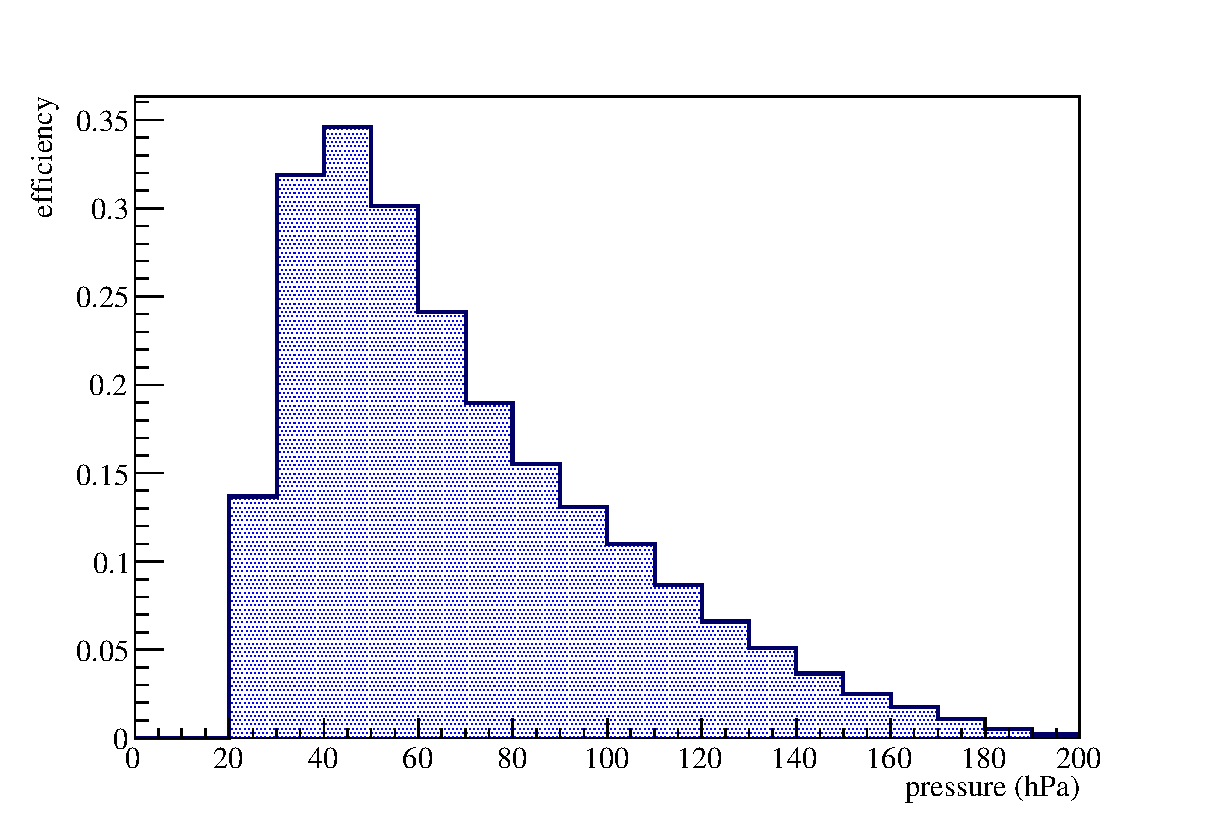
\includegraphics[clip, width=0.8\columnwidth]{efficiency_P_dist.eps}
  \caption[\Methane の圧力による検出効率の分布.]
          {\Methane の圧力による検出効率の分布.
            $\alpha$粒子は図\ref{fig::alpha_E_dist}に示したエネルギー分布を仮定した.
           }
  \label{fig::efficiency_P_dist}
\end{figure}
\SI{50}{\hecto\pascal}のときの\Methane の各種の値は表\ref{tab::CH4_50_params}のとおりである.
\begin{table}
  \centering
  \caption{\SI{50}{\hecto\pascal}のときの\Methane のパラメータ.}
  \label{tab::CH4_50_params}
  \begin{tabular}{cc}
    \toprule
    項目 & 値\\
    \midrule
    密度 & \SI{3.29e-5}{\gram\per\cubic\centi\metre} \\
    $dE/dx$ ($E_{\alpha} = \SI{0.5}{\mega\electronvolt}$, \SI{10}{\milli\metre}) & \SI{0.107}{\mega\electronvolt}\\
    飛距離 ($E_{\alpha} = \SI{0.5}{\mega\electronvolt}$) & \SI{65.6}{\milli\metre} \\
    検出率 & \SI{48.2}{\percent} \\
    \bottomrule
  \end{tabular}
\end{table}
\begin{table}
  \centering
  \caption[ガスの混合パターン,圧力,$dE/dx$.]
          {ガスの混合パターン,圧力,$dE/dx$.
          括弧内はガスの混合の割合を示す.}
  \label{tab::mixture}
  \begin{tabular}{ccccc}
    \toprule
    gas &
    \begin{tabular}{c}
      pressure \\
      (\si{\hecto\pascal})
    \end{tabular} &
    \begin{tabular}{c}
      density \\
      (\si{\gram\per\cubic\centi\metre})
    \end{tabular} &
    \begin{tabular}{c}
      $dE/dx$ (\si{\mega\electronvolt})\\
      $E_{\alpha} = \SI{0.5}{\mega\electronvolt}$ \\
      \SI{10}{\milli\metre}
    \end{tabular} &
    \begin{tabular}{c}
      ドリフト電場 (\si{\volt\per\milli\metre}) \\
      @ \SI{0.014}{\milli\metre\per\nano\second}
    \end{tabular}\\
    \midrule
    \Methane         & 50  & 3.29$\times 10^{-5}$ & 0.107 & 0.418 \\
    \MethaneHydro    & 100 & 2.55$\times 10^{-5}$ & 0.107 & 4.31 \\
    \MethaneHerium   & 100 & 3.62$\times 10^{-5}$ & 0.109 & 1.89 \\
    \isoButane       & 15  & 3.58$\times 10^{-5}$ & 0.102 & 0.644 \\
    \isoButaneHydro  & 100 & 3.13$\times 10^{-5}$ & 0.122 & 6.80 \\
    \isoButaneHerium & 100 & 3.86$\times 10^{-5}$ & 0.102 & 3.26 \\
    \bottomrule
  \end{tabular}
\end{table}

\subsection{ドリフトスピード}
MAIKo TPC では\SI{100}{\mega\hertz}で1,024 samples データを取得するため,
ドリフト方向は\SI{10.24}{\micro\second}のタイムウィンドウが開いている.
ドリフトケージの大きさ (\SI{140}{\milli\metre}) を可能な限りタイムウィンドウに収めるためには,
ドリフトスピードを$\SI{140}{\milli\metre}/\SI{10.24}{\micro\second} \sim \SI{0.014}{\milli\metre\per\nano\second}$
に調整する必要がある.
Magboltz~\cite{magboltz} によって計算したドリフト電場とドリフトスピードの関係を図\ref{fig::drift_v_magboltz}に示す.
ドリフトスピードが\SI{0.014}{\milli\metre\per\nano\second}となるドリフト電場の値を表\ref{tab::mixture}に示す.
図\ref{fig::drift_v_magboltz}の横方向の点線は\SI{0.014}{\milli\metre\per\nano\second}を表す.
以降,これらのドリフト電場で評価を行う.
\begin{figure}
  \centering
  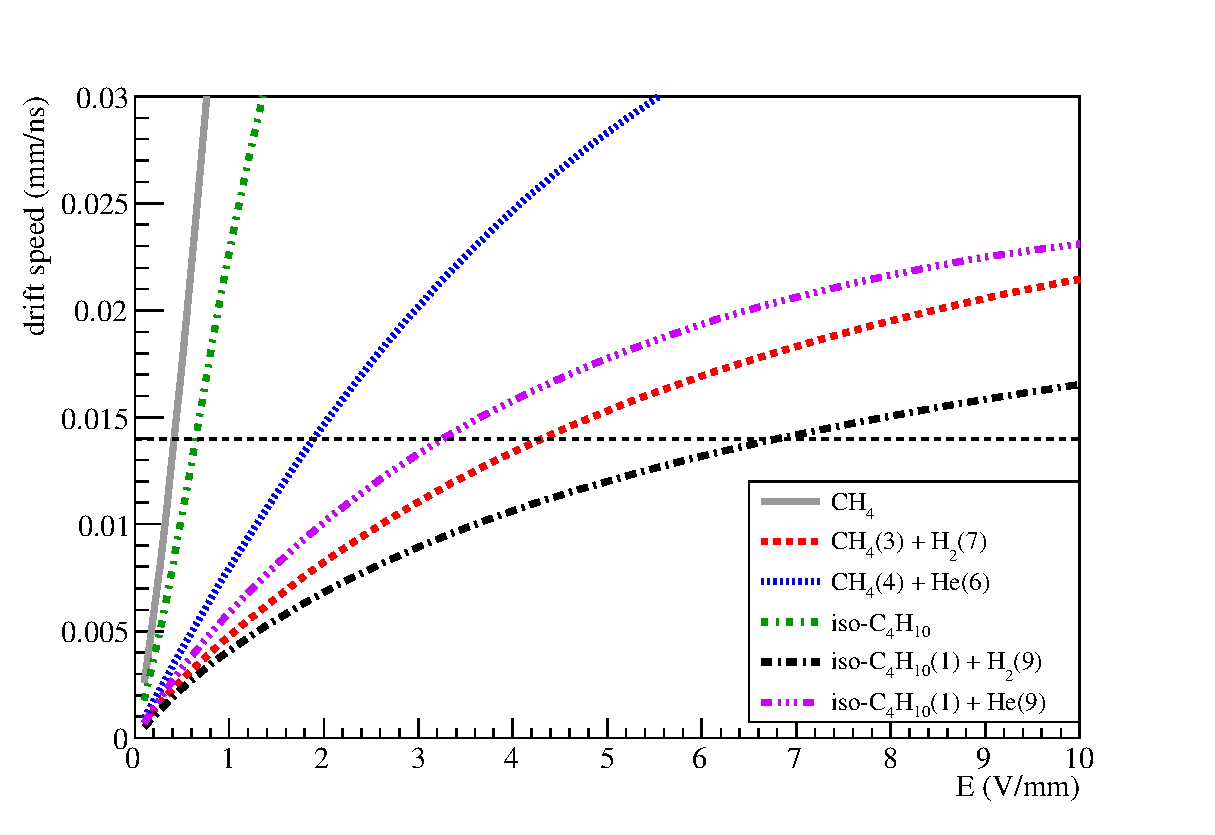
\includegraphics[clip, width=0.9\columnwidth]{drift_v_magboltz.eps}
  \caption[ドリフト電場とドリフトスピードの関係.]
          {ドリフト電場とドリフトスピードの関係.
            \Methane は\SI{50}{\hecto\pascal},\isoButane は\SI{15}{\hecto\pascal},その他は\SI{100}{\hecto\pascal}である.
            横方向の点線は\SI{0.014}{\milli\metre\per\nano\second}を示す.}
          \label{fig::drift_v_magboltz}
\end{figure}

\subsection{電子のディフュージョンの効果}
ドリフト電場によって電子が移動する間に検出ガスとの散乱と電子の熱運動により,
図\ref{fig::diffusion-image}のように広がりながらドリフトする.
電子が広がることをディフュージョンと呼ぶ.
この効果が大きくなると,
荷電粒子によって同じ場所に生成された電子が$\mu$-PICに到達するまでに広がるため,
トラックが太く検出される.
トラックが太くなると,複数のトラックを分離することが難しくなる.
そのため,ディフュージョンの効果が小さいことが望まれる.
\begin{figure}
  \centering
  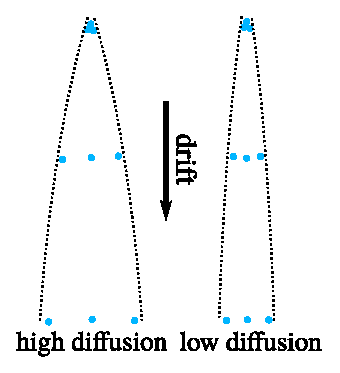
\includegraphics[clip, width=0.4\columnwidth]{diffusion_image.eps}
  \caption[ディフュージョンによって電子が拡散するイメージ.]
          {ディフュージョンによって電子が拡散するイメージ.
          同じ位置で生成された電子でもドリフトする間に位置が拡散する.}
  \label{fig::diffusion-image}
\end{figure}

ドリフト電場がない場合のディフュージョンは以下のように理解できる.
電子は熱運動により発生点から拡散する.
熱運動の平均速度$v$はMaxwell 分布より
\begin{equation}
  v = \sqrt{\frac{8k_{B}T}{\pi \si{\electronmass}}}
  \label{eq::maxwell_velocity}
\end{equation}
と表せる.
ここで$k_{B}$はボルツマン定数,$T$は温度,\si{\electronmass}は電子の質量である.
電子が発生した時刻から$\Delta t$後では,
\begin{equation}
  \frac{N_0}{\sqrt{4\pi D t}}\exp\left(-\frac{x^{2}}{4 D t}\right)
  \label{eq::gaus_dist}
\end{equation}
のガウス分布で電子が広がる.
ここで$N_{0}$は全粒子数,$x$は発生した点からの距離,$D$はディフュージョン係数を表す.
ディフュージョン係数$D$は電子の平均自由工程$\lambda$を用いて
\begin{equation}
  D = \frac{1}{3}v\lambda
  \label{eq::diffusion_coef}
\end{equation}
と表せる.
理想気体において平均自由工程$\lambda$は,ガスとの散乱の全断面積$\sigma_{0}$,圧力$p$のもとで
\begin{equation}
  \lambda = \frac{1}{\sqrt{2}}\frac{k_{B}T}{\sigma_{0}p}
  \label{eq::lambda}
\end{equation}
と表される.
式\ref{eq::maxwell_velocity}, \ref{eq::diffusion_coef}, \ref{eq::lambda}により,
\begin{equation}
  D = \frac{2}{3\sqrt{\pi}}\frac{1}{p\sigma_{0}}\sqrt{\frac{\left(k_{B}T\right)^{3}}{\si{\electronmass}}}
  \label{eq::diffusion_coef_2}
\end{equation}
となる.
式\ref{eq::diffusion_coef_2}より,
同じガスでは圧力が高いほど,温度が低いほどディフュージョン係数が小さいことが分かる.

ドリフト電場がある場合,発生点からの距離を$L$,ドリフトスピードを$v_{\text{drift}}$とすると,
\begin{equation}
  \Delta t = \frac{L}{v_{\text{drift}}}
  \label{eq::delta_t}
\end{equation}
となる.
式\ref{eq::gaus_dist}の分散$\sigma(L)$は
\begin{align}
  \sigma(L) & = \sqrt{2 D \Delta t}\\
  & = \sqrt{\frac{2 D}{v_{\text{drift}}}}\times\sqrt{L}\\
  & = D_{\rm Magboltz}\times\sqrt{L}
\end{align}
となる.
Magboltz によってディフュージョン係数$D_{\rm Magboltz}$が得られる.
Magboltz によって計算したディフュージョン係数を表\ref{tab::diffusion}に示す.
表\ref{tab::diffusion}中の$D_{t}$はドリフト方向に対して垂直な方向への拡散,$D_{l}$は電子の運動方向への拡散の係数を表す.
\Methane および\isoButane の単体ではディフージョン係数が大きく,
同じドリフトスピードのとき,ドリフト電場が大きいほどディフュージョン係数が小さいことが分かる.
\isoButaneHydro が最もディフュージョン係数が小さく,
検出ガスの最有力候補である.
シミュレーションにより生成した${}^{12}{\rm C}({\rm n},{\rm n}'){}^{12}{\rm C} (0_2^+)$イベントを解析し,
その解析効率により検出ガスを決定する.
\begin{table}
  \centering
  \caption[Magboltz で計算したディフュージョンの係数.]
          {Magboltz で計算したディフュージョンの係数.
            ディフージョンの大きさはドリフト電場に依存するため,
            ここではドリフトスピードが\SI{0.014}{\milli\metre\per\nano\second}になるドリフト電場での値を示す.
          $D_{t}$,$D_{l}$はそれぞれ運動方向に垂直,平行方向のディフュージョン.}
  \label{tab::diffusion}
  \begin{tabular}{cccc}
    \toprule
    gas & $D_{t}$(\si{\sqrt{\milli\metre}}) & $D_{l}$(\si{\sqrt{\milli\metre}}) &
    ドリフト電場 (\si{\volt\per\milli\metre}) \\
    \midrule
    \Methane & 0.433 & 0.547 & 0.418\\
    \MethaneHydro & 0.214 & 0.171 & 4.31\\
    \MethaneHerium & 0.270  & 0.248 & 1.89\\
    \isoButane & 0.357 & 0.414 & 0.644\\
    \isoButaneHydro & 0.196 & 0.145 & 6.80\\
    \isoButaneHerium & 0.246 & 0.197 & 3.26\\
    \bottomrule
  \end{tabular}
\end{table}

%\section{$\alpha$線源を用いた測定}
%$\alpha$線源を用いてMAIKo TPC の動作確認を行う.
%線源では,電子のドリフトスピード,増幅率,トラックの太さを確認する.

%\subsection{HV系}
%%ここでは電圧の変数名を説明する.
%
%\subsection{ガス系}
%
%\subsection{回路系}
%

%ドリフト速度の決定方法は30 degree 方向に$\alpha$線源から$\alpha$を出して,
%その飛跡がデータ上でどう見えるかで決定する.
%ドリフト速度の時間依存性も見た.

%\section{中性子カウンター (液体シンチレータ)}
%\subsection{キャリブレーション}
%\subsection{波形弁別}
%\subsection{検出効率}
%
%\section{中性子カウンター (金属箔)}
%

\end{document}

%\documentclass[master]{subfiles}

\begin{document}

\chapter{OKTAVIAN}
\section{OKTAVIAN}
大阪大学強力14MeV中性子工学実験装置 (OKTAVIAN) によって生成した単色中性子ビームを用いて
${}^{12}\rm{C}(n,n'){}^{12}\rm{C}(0_{2}^{+})$の断面積の測定を行う。
中性子の発生には
\begin{equation}
  t(d,{}^{4}\rm{He})n
\end{equation}
反応を用いる。
この反応を用いることにより、
およそ$14\rm{MeV}$の単色中性子を発生させることが可能となる。

コッククロフト・ワルトン型加速装置を用いることで、
デューテリウムを加速しトリチウム標的に照射する。
OKTAVIANには連続照射ラインとパルスラインの2つのビームラインがある。
パルスラインでは$1\rm{kHz}$--$2\rm{MHz}$のパルス状の
ビームを照射することができる。
ビーム電流は時間平均で$6.67\rm{p\mu A}$である。
連続照射ラインでは連続的にビームを小差hすることができ、
ビーム電流は$6.67\rm{pmA}$である。
ビームの時間情報を用いて解析を行うことが可能となるが、
パルスビームラインのトリチウム標的は実験室内にあり、
コリメートされていない中性子を用いることになる。
この場合、実験室の壁などに反跳した中性子がバックグランドになるため、
本実験には適していない。
そのため、この実験では連続照射ラインを使用する。
連続照射ラインを用いる場合、
重照射室においてデューテリウムビームをトリチウム標的に照射し、
大実験室との間にある穴から中性子ビームの取り出しを行う。

\subsection{MAIKo架台}
中性子のバックグラウンドを低減させるため、
実験装置は可能な限り取り出し穴に近づける必要がある。
しかし、取り出し穴のあるは階段上にあるため、
階段の上に実験装置を設置することとなる。

\section{中性子ビーム}
\subsection{コリメータ}
\subsection{ビーム量およびエネルギー}

\end{document}

\documentclass[../master]{subfiles}

%\graphicspath{{../eps/}}

\begin{document}

\chapter{シミュレーションによるトラックの再現}
\label{chap::simulation}
\section{\texorpdfstring{$\alpha$}{alpha}線源を用いた測定}
\ref{sec::detection_gas_candidate}節で考えた各検出ガスについて,
実際に$\alpha$線源から放出される$\alpha$粒子のトラックを測定した.
また,それらのデータから各ガスにおけるドリフト速度,ガスの電子増幅率,トラックの幅を決定した.
測定には${}^{241}{\rm Am}$の$\alpha$線源を用いた.
図\ref{fig::a_source_track}に$\alpha$線源のトラックの一例を示す.
図\ref{fig::a_source_track}では検出ガスに\SI{100}{\hecto\pascal}の\isoButaneHydro を用いた.
\ref{sec::detection_gas_candidate}節では6種類の候補を考えたが,
ここからは単体のiso-$\rm C_{4}H_{10}$を除いた5種類について考えていく.
これは単体の\isoButane を検出ガスに用いた場合に,
拡散係数が大きくトラックが太くなると予測されることと,
圧力が\SI{15}{\hecto\pascal}と低く安定したTPC の動作が難しいと予測されるためである.
\begin{figure}
  \centering
  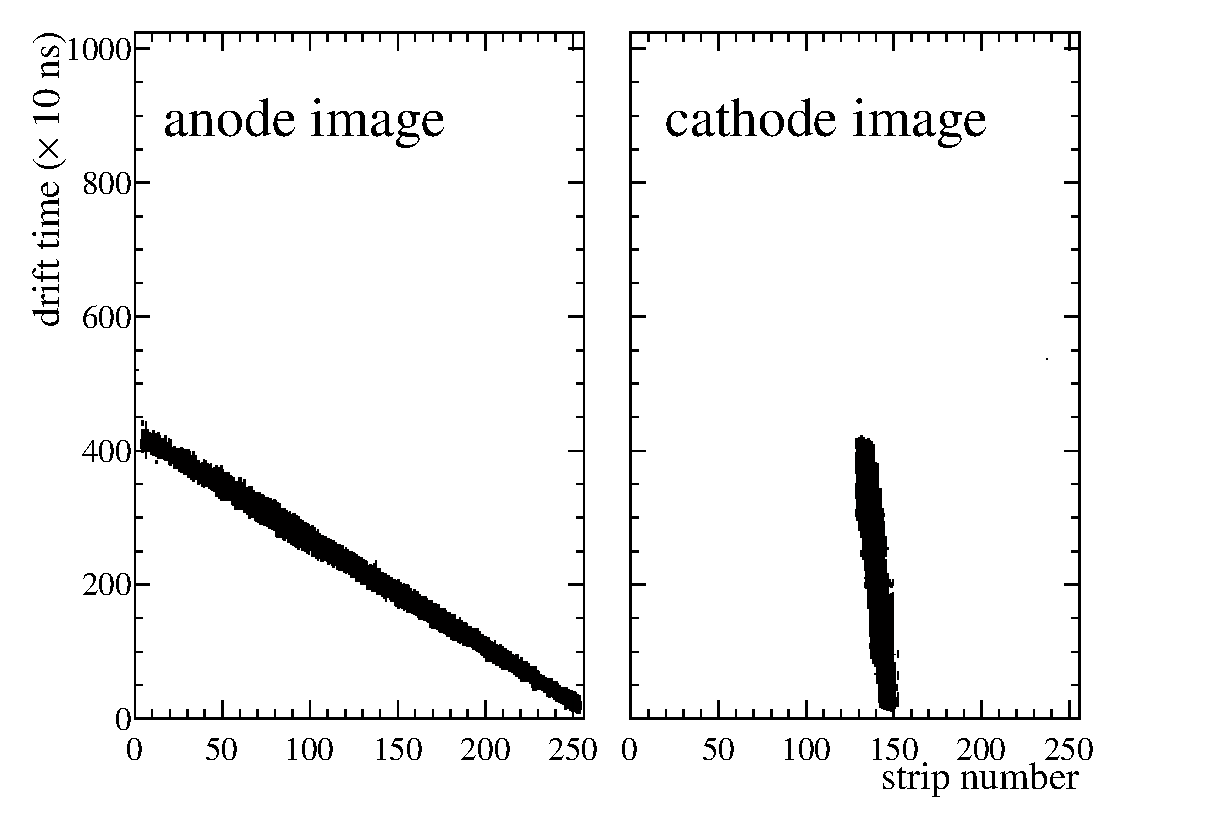
\includegraphics[clip, width=0.9\columnwidth]{0210_7.eps}
  \caption[$\alpha$粒子を測定したトラックの一例.]
          {$\alpha$粒子を測定したトラックの一例.
          検出ガスには\isoButaneHydro を用いた.}
  \label{fig::a_source_track}
\end{figure}

\subsection{ドリフト速度の測定}
電子のドリフト速度を線源によって得られるトラックから実測する.
測定には図\ref{pic::alpha_collimator}のような線源コリメータを用いる.
このコリメータはアクリルで作られており,1つの\ang{0}と4つの\ang{30}の穴が設けられている.
このコリメータを用いることで$\alpha$線の放出方向を\ang{0}と\ang{30}の方向に限定することができる.
\ang{30}方向の$\alpha$線は図\ref{fig::drift_v_image}の右のようにドリフト方向に$\Delta y$~\si{\milli\metre},
それと垂直な方向に$\Delta z$~\si{\milli\metre}移動するとき,
\begin{equation}
  \Delta y = \tan(\ang{30})\times\Delta z \label{eq::deltay_deltaz}
\end{equation}
となる.
MAIKo TPC で取得したトラックの横方向の変分を$\Delta strip$,縦方向の変分を$\Delta t$~\si{\nano\second},
ドリフト速度を$v_{\text{drift}}$~\si{\milli\metre\per\nano\second}とすると,
\begin{align}
  \frac{\Delta z}{\SI{0.4}{\milli\metre}} & = \Delta strip \label{eq::deltaz}\\
  \frac{\Delta y}{v_{\text{drift}}} & = \Delta t \label{eq::deltay}
\end{align}
という関係にある.
式\eqref{eq::deltay_deltaz}, \eqref{eq::deltaz}, \eqref{eq::deltay} より
\begin{equation}
  v_{\text{drift}} = \frac{\tan(\ang{30})\times\Delta strip\times\SI{0.4}{\milli\metre}}{\Delta t}
\end{equation}
とドリフト速度が決定される.
\begin{figure}
  \centering
  \begin{subfigure}{0.45\columnwidth}
    \centering
    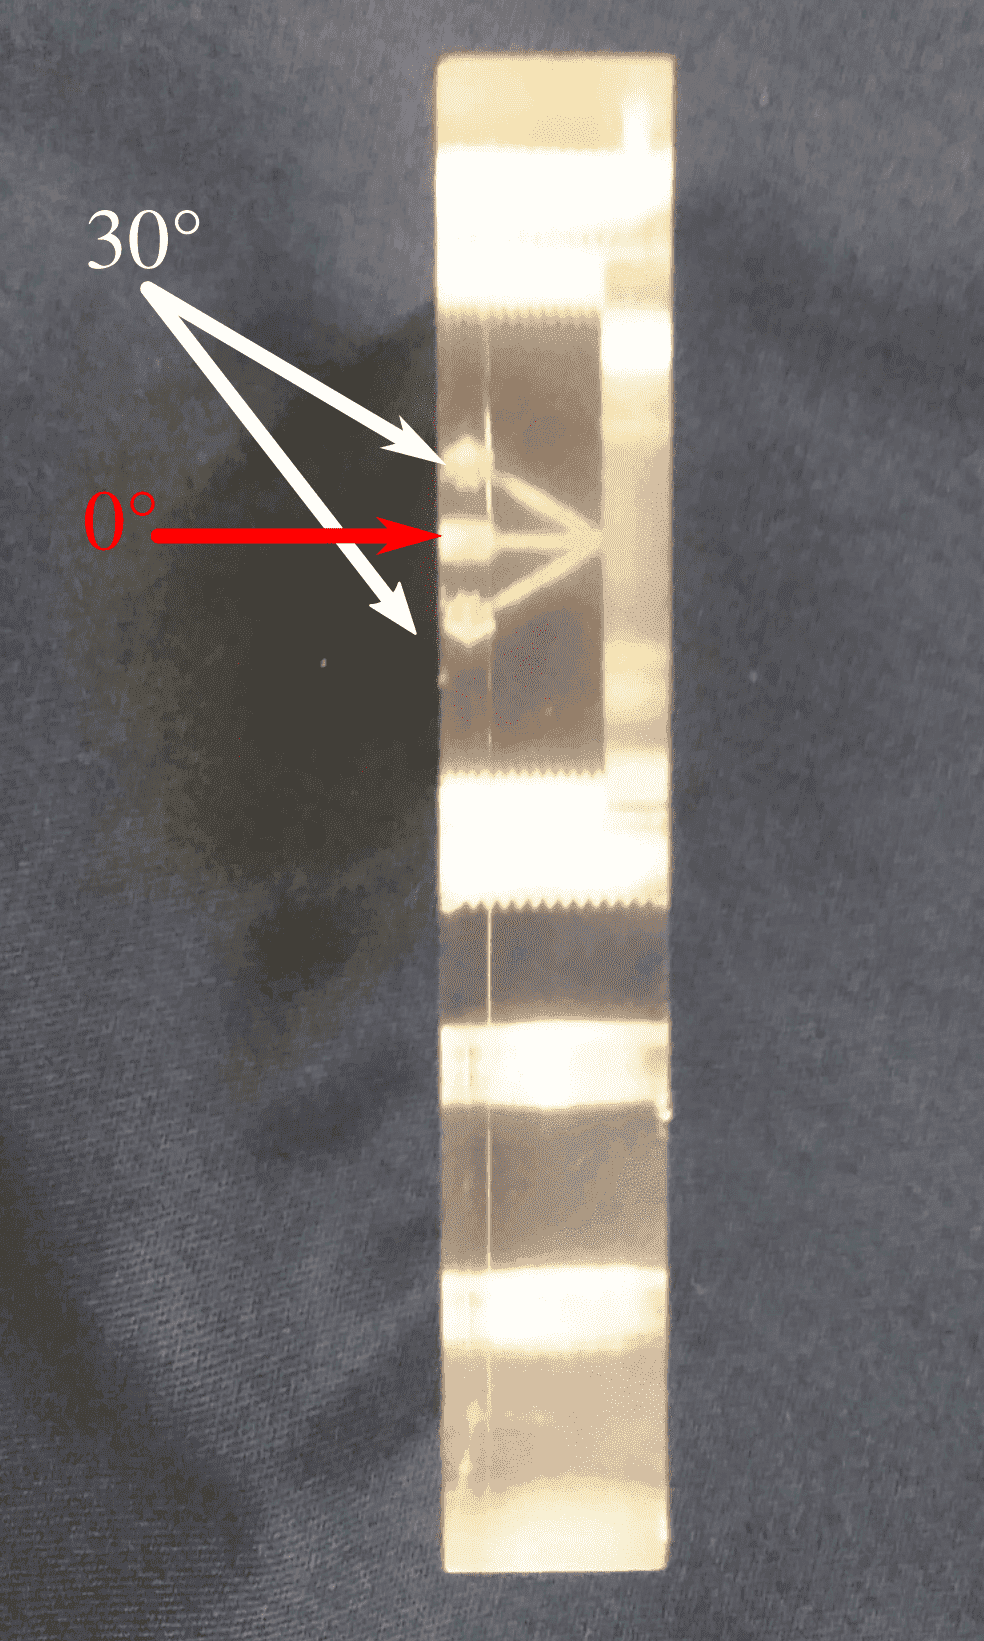
\includegraphics[clip, width=0.8\columnwidth]{image30580-min.png}
    \caption{側面.}
  \end{subfigure}
  \begin{subfigure}{0.45\columnwidth}
    \centering
    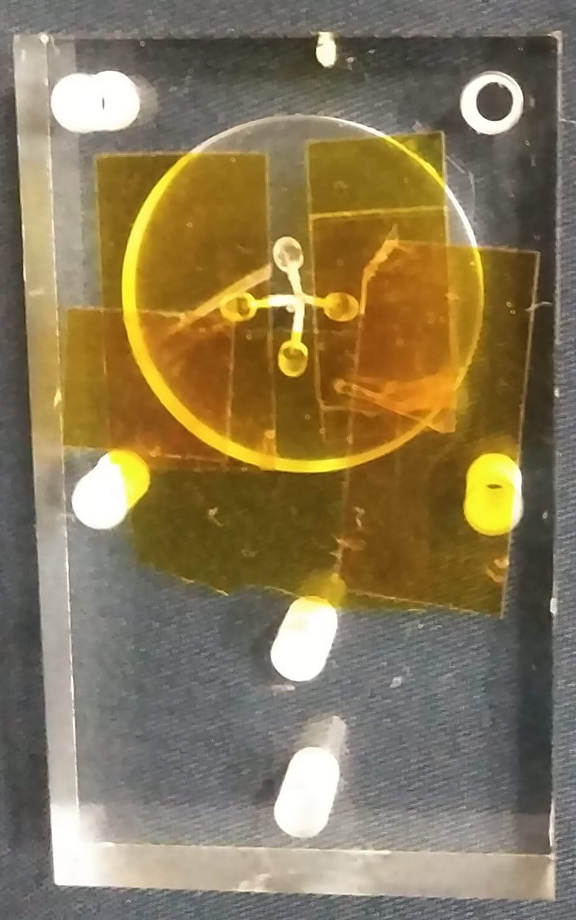
\includegraphics[clip, width=0.8\columnwidth]{IMG_20191225_183542_clip.jpg}
    \caption{正面.}
  \end{subfigure}
  \caption[線源コリメータ.]
          {線源コリメータ.中央に\ang{0},上下左右に\ang{30}の穴が設けられている.
            \ang{0}の穴と1つの\ang{30}の穴を除いてカプトンテープで封じることにより,
            $\alpha$先の放出方向を限定している.
          }
          \label{pic::alpha_collimator}
\end{figure}
\begin{figure}
  \centering
  \begin{minipage}{0.45\columnwidth}
    \centering
    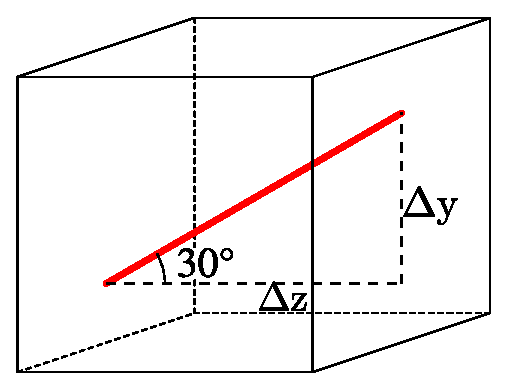
\includegraphics[clip, width=0.9\columnwidth]{drift_v_source.eps}
  \end{minipage}
  \begin{minipage}{0.45\columnwidth}
    \centering
    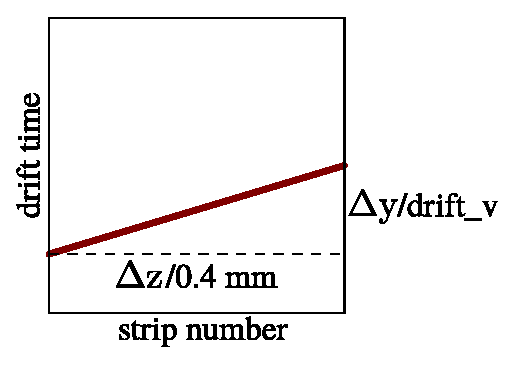
\includegraphics[clip, width=\columnwidth]{drift_v_image.eps}
  \end{minipage}
  \caption[\ang{30}に方向を限定した$\alpha$線と取得される画像データのイメージ.]
          {\ang{30}に方向を限定した$\alpha$線 (左) と取得される画像データ (右) のイメージ.}
  \label{fig::drift_v_image}
\end{figure}

$\alpha$線源を用いて測定したドリフト速度とMagboltz で計算した値を
表\ref{tab::drift_speed_compare}に示す.
$\alpha$線源を用いて測定したドリフト速度と Magboltz を用いて計算したドリフト速度が概ね一致していることが分かる.
ここで,Magboltz の計算値が\SI{0.014}{\milli\metre\per\nano\second}となっていないのは,
MAIKo TPC の実際の運用を簡単にするために設定電圧を切りの良い値にしたためである.
\Methane は実測とMagboltz による計算値に不一致が見られるが,
\Methane のみ\SI{50}{\hecto\pascal} とその他のガスと比較して圧力が半分であるため,
不純物,特に水分の影響を強く受けていると考えられる.
水分のドリフト速度へ与える影響は付録\ref{app::drift_speed_humid_dep}で述べる.
\begin{table}
  \centering
  \caption{実測したドリフト速度とMagboltz を用いて計算したドリフト速度の比較.}
  \label{tab::drift_speed_compare}
  \begin{tabular}{cccc}
    \toprule
    gas & ドリフト電場 (\si{\volt\per\milli\metre}) & 実測値 (\si{\milli\metre\per\nano\second})
    & 計算値 (\si{\milli\metre/\nano\second})\\
    \midrule
    \Methane & 0.429 & 0.0126 & 0.0145 \\
    \MethaneHydro & 4.32 & 0.0140 & 0.0140 \\
    \MethaneHerium & 1.89 & 0.0135 & 0.0140 \\
    \isoButaneHydro & 6.82 & 0.0137 & 0.0140 \\
    \isoButaneHerium & 3.29 & 0.0139 & 0.0141 \\
    \bottomrule
  \end{tabular}
\end{table}
%\begin{figure}
%  \centering
%  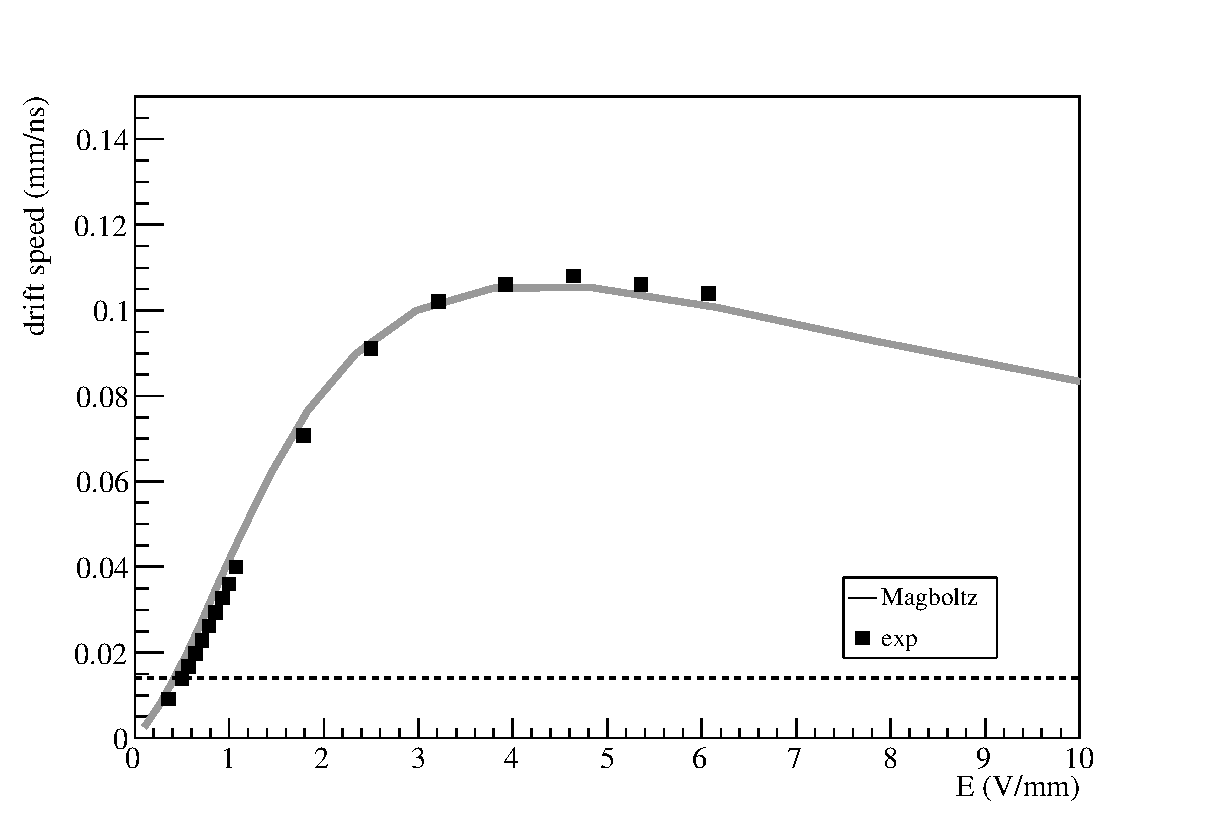
\includegraphics[clip, width=0.9\columnwidth]{drift_v_CH4.eps}
%  \caption[検出ガスに${\rm CH_{4}}$を用いたときのドリフトスピードの電場依存性.]
%          {検出ガスに${\rm CH_{4}}$を用いたときのドリフトスピードの電場依存性.
%            図中の点線は0.014 mm/ns を示す.}
%  \label{fig::drift_v_CH4}
%%  \includegraphics[clip, width=0.7\columnwidth]{drift_v_CH4_H2.eps}
%  \caption{}
%  \label{fig::drift_v_CH4_H2}
%%  \includegraphics[clip, width=0.7\columnwidth]{drift_v_CH4_He.eps}
%  \caption{}
%  \label{fig::drift_v_CH4_He}
%  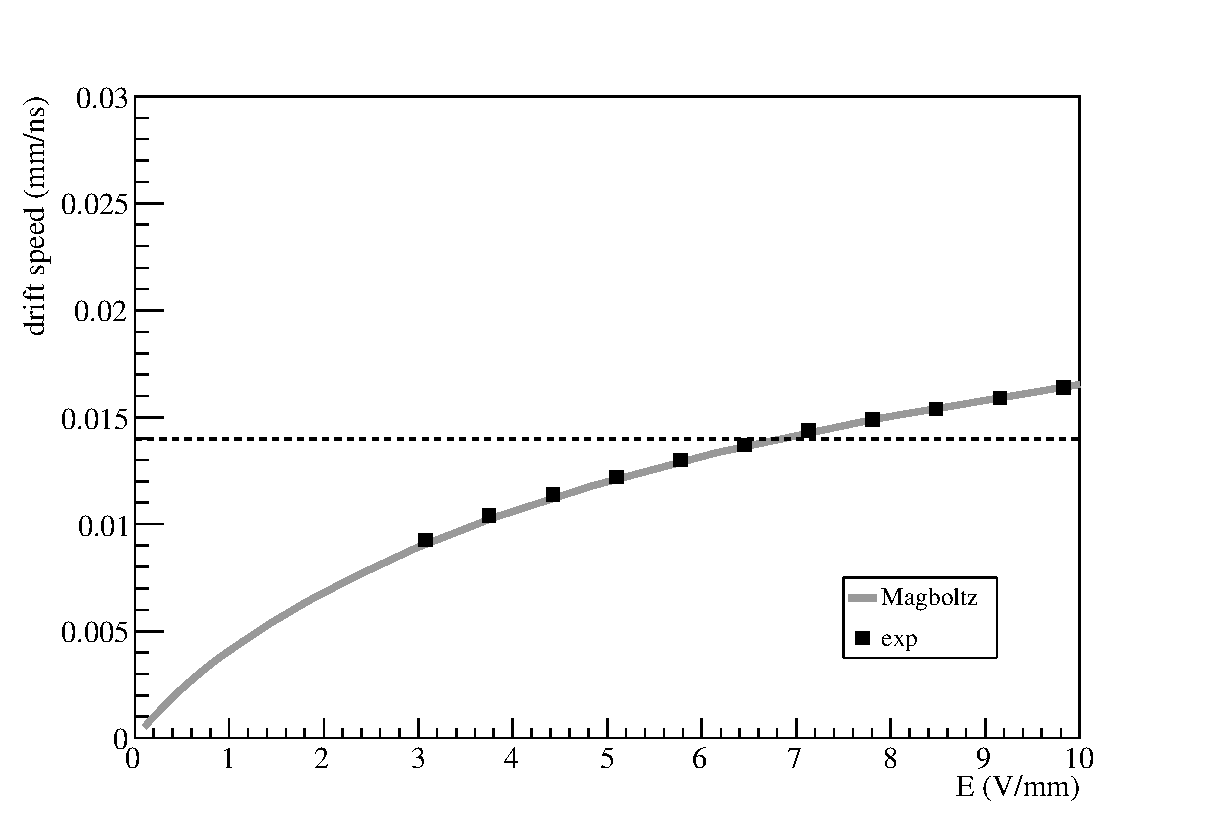
\includegraphics[clip, width=0.9\columnwidth]{drift_v_iC4H10_H2.eps}
%  \caption[検出ガスにiso-${\rm C_{4}H_{10}}$を用いたときのドリフトスピードの電場依存性.]
%          {検出ガスにiso-${\rm C_{4}H_{10}}$を用いたときのドリフトスピードの電場依存性.
%        p    図中の点線は0.014 mm/ns を示す.}
%  \label{fig::drift_v_iC4H10_H2}
%%  \includegraphics[clip, width=0.7\columnwidth]{drift_v_iC4H10_He.eps}
%  \caption{}
%  \label{fig::drift_v_iC4H10_He}
%\end{figure}

\subsection{電子増幅率}
%各部の電圧に対する電子増幅率の依存性を測定した.
GEM および$\mu$-PICによる電子の増幅率を測定した.
増幅率は荷電粒子が検出ガス中を通過した際に発生させた電子数 ($N_{\mathrm{e}}$) と
増幅後に$\mu$-PICによって収集された電子数 ($N'_{\mathrm{e}}$) から求めることができる.
$N_{\mathrm{e}}$は検出ガス中での荷電粒子のエネルギー損失と検出ガスのW値(1つの電子対の生成に必要なエネルギー)から求める.
$N'_{\mathrm{e}}$は$\mu$-PICで収集した電荷から求める.
%詳しい計算方法について以下で述べる.
%
検出ガス中で荷電粒子がエネルギーを損失すると,W値あたり平均1個の電子を電離する.
そのため,荷電粒子のエネルギー損失をW値で除することで$N_{\mathrm{e}}$が求まる.
各検出ガスにおけるエネルギー損失とW値~\cite{energy_per_ion_pair,pdg}を表\ref{tab::energy_loss_and_W_val}に示す.
本研究ではでは${}^{241}\mathrm{Am}$からの$\alpha$線を用いて測定を行った.
${}^{241}\mathrm{Am}$からは\SI{5.48}{\mega\electronvolt}の$\alpha$線が放出される.
今回の測定に用いた$\alpha$線源は線量を大きくするために,多くの${}^{241}\mathrm{Am}$が線源に含まれている.
そのため,物質厚が大きくなっており,$\alpha$線が放出される前に線源中でエネルギーを損失してしまう.
この線源から出ている$\alpha$粒子の持つエネルギーが平均\SI{4.2}{\mega\electronvolt}であることが過去の測定により確認している.
今回の測定では\ang{0}方向に放出された$\alpha$線を用いて測定した.
エネルギー損失は\SI{4.2}{\mega\electronvolt}の$\alpha$粒子が$\mu$-PIC 32 strip分の
距離 (\SI{12.8}{\milli\metre}) で落とすエネルギーを示している.
この距離で発生した電子が$\mu$-PIC の32 stripsで収集される.
\begin{table}
  \centering
  \caption[検出ガスのW値とエネルギー損失と$N_{\rm e}$.]
          {検出ガスのW値~\cite{energy_per_ion_pair,pdg}とエネルギー損失と$N_{\rm e}$.
          エネルギー損失は\SI{4.2}{\mega\electronvolt}の$\alpha$粒子が
          ガス中を\SI{12.8}{\milli\metre} 進んだ時の値である.}
  \label{tab::energy_loss_and_W_val}
  \begin{tabular}{cccc}
    \toprule
    gas & W値 (\si{\electronvolt}) & energy loss (\si{\kilo\electronvolt}) & $N_{\rm e}$\\
    \midrule
    \Methane         & 29.1 & 56.5 & 1.94$\times 10^{3}$ \\
    \MethaneHydro    & 34.2 & 53.4 & 1.56$\times 10^{3}$ \\
    \MethaneHerium   & 39.2 & 59.3 & 1.51$\times 10^{3}$ \\
%    iso-${\rm C_{4}H_{10}}$                 & 26.0 & 0.0552 & 2.12$\times 10^{3}$ \\
    \isoButaneHydro  & 35.4 & 62.0 & 1.75$\times 10^{3}$ \\
    \isoButaneHerium & 44.0 & 58.0 & 1.32$\times 10^{3}$ \\
    \bottomrule
  \end{tabular}
\end{table}

32 strips まとめた$\mu$-PICからの信号波形は図\ref{fig::FADC_waveform}のようなFADC 情報として取得している.
この信号波形を時間で積分することによって32 strips で収集した電荷量を計算することができる.
$\mu$-PICで取得した電気信号は読み出し回路内部で800倍に増幅され,
FADC の入力インピーダンス\SI{50}{\ohm}で電流値を電圧値に変換して取得している.
よって,式\eqref{eq::N'e}で$\mu$-PICで収集した電荷量を得ることができる.
\si{\elementarycharge}は電気素量である.
\begin{equation}
  N'_{\mathrm{e}} = \frac{\int V (t) dt}{ 50 \times 800 \times \si{\elementarycharge}}
  \label{eq::N'e}
\end{equation}
各検出ガスの増幅率と電子の収集効率を畳み込んだ値を表\ref{tab::multiplying_rate}に示す.
ここでは,GEMと$\mu$-PIC の両方による増幅率となっている.
また,測定時のGEM や$\mu$-PICに印加した電圧を表\ref{tab::high_voltage_config_for_gain_meas}に示す.
\begin{table}
  \centering
  \caption{各検出ガスの電子増幅率.}
  \label{tab::multiplying_rate}
  \begin{tabular}{cc}
    \toprule
    gas & 増幅率 (倍) \\
    \midrule
    \Methane         & 700 \\
    \MethaneHydro    & 354 \\
    \MethaneHerium   & 322 \\
    \isoButaneHydro  & 272 \\
    \isoButaneHerium & 392 \\
    \bottomrule
  \end{tabular}
\end{table}
\begin{table}
  \caption{電子増幅率を測定した際の電圧設定.GEM のうちgrid 側をGEMt,$\mu$-PIC側をGEMbとする.}
  \label{tab::high_voltage_config_for_gain_meas}
  \centering
  \begin{tabular}{cccccc}
    \toprule
    gas & plate (\si{\volt}) & grid (\si{\volt}) & GEMt (\si{\volt}) & GEMb (\si{\volt}) & $\mu$-PIC (\si{\volt}) \\
    \midrule
    \Methane         & $-1370$ & $-1290$ & $-560$ & $-150$ & $175$ \\
    \MethaneHydro    & $-2105$ & $-1500$ & $-620$ & $-250$ & $420$ \\
    \MethaneHerium   & $-1465$ & $-1200$ & $-600$ & $-250$ & $400$ \\
    \isoButaneHydro  & $-2255$ & $-1300$ & $-600$ & $-250$ & $400$ \\
    \isoButaneHerium & $-1430$ & $-970$ & $-600$ & $-250$ & $300$ \\
    \bottomrule
  \end{tabular}
\end{table}

\subsection{トラックの幅}
本実験の目的である3$\alpha$に崩壊するイベントでは観測されるトラックが太いと複数のトラックの区別が難しくなり,
トラックを正しく抽出できなくなる.
そこで,\ang{0}の$\alpha$粒子によるトラックの幅を測定した.
図\ref{fig::track_width}に示すように,
トラックの幅にはanode strip 128~ch目のclock方向の幅を用いる.
このようにして決定したトラックの幅を%表\ref{tab::track_width},
図\ref{fig::diffusion_compare}に示す.
図\ref{fig::diffusion_compare}から分かるようにトラックの幅と拡散係数には相関がある.
拡散係数,トラックの幅ともに\isoButaneHydro が最も小さいことが分かる.
\begin{figure}
  \centering
  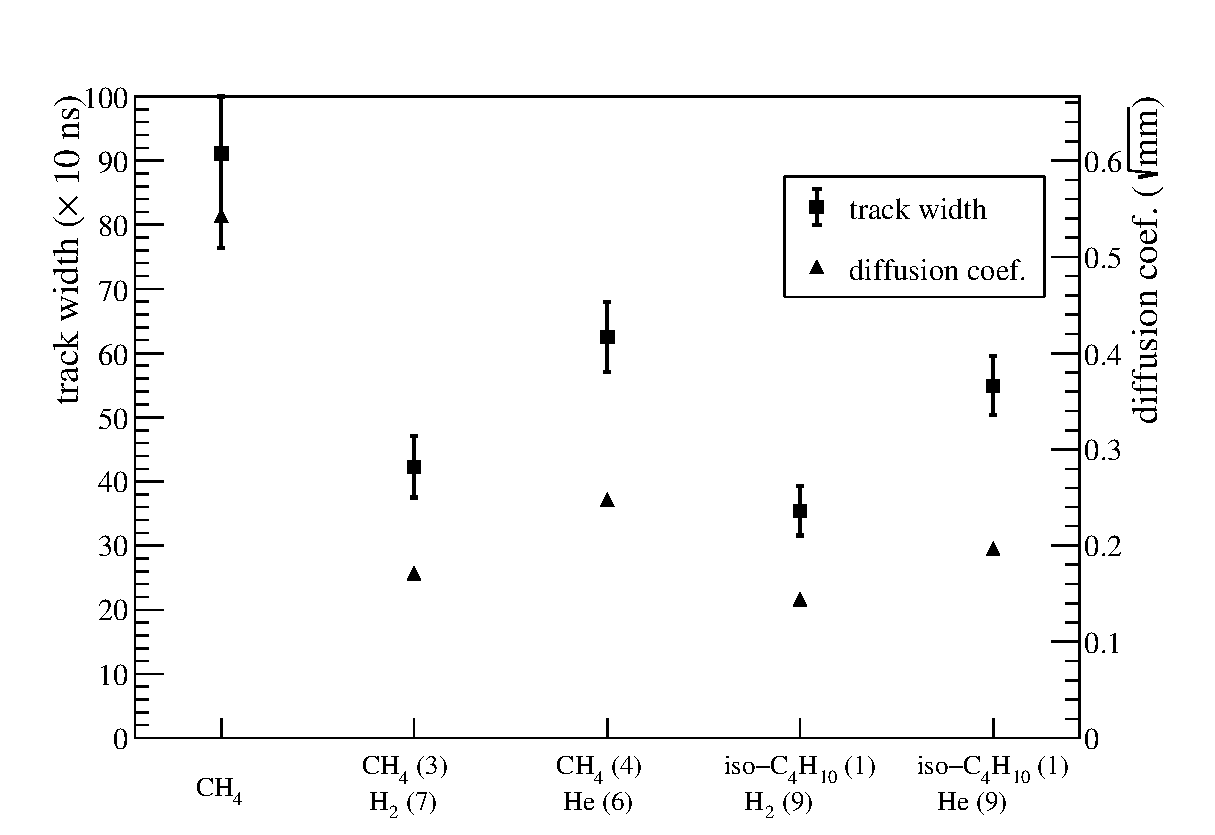
\includegraphics[clip, width=0.8\columnwidth]{track_width.eps}
  \caption{トラックの幅の決定方法のイメージ.
    トラックの幅は有感領域の中央であるanode strip 128~chのclock方向の幅を用いる.}
  \label{fig::track_width}
\end{figure}

%\begin{table}
%  \centering
%  \caption{各検出ガスでのトラックの幅.}
%  \label{tab::track_width}
%  \begin{tabular}{cc}
%    \toprule
%    gas & トラックの幅 ($\times \SI{10}{\nano\second}$)\\
%    \midrule
%    \Methane         & 91.1 \\
%    \MethaneHydro    & 42.3 \\
%    \MethaneHerium   & 62.5 \\
%    \isoButaneHydro  & 35.4 \\
%    \isoButaneHerium & 54.9 \\
%    \bottomrule
%  \end{tabular}
%\end{table}

\begin{figure}
  \centering
  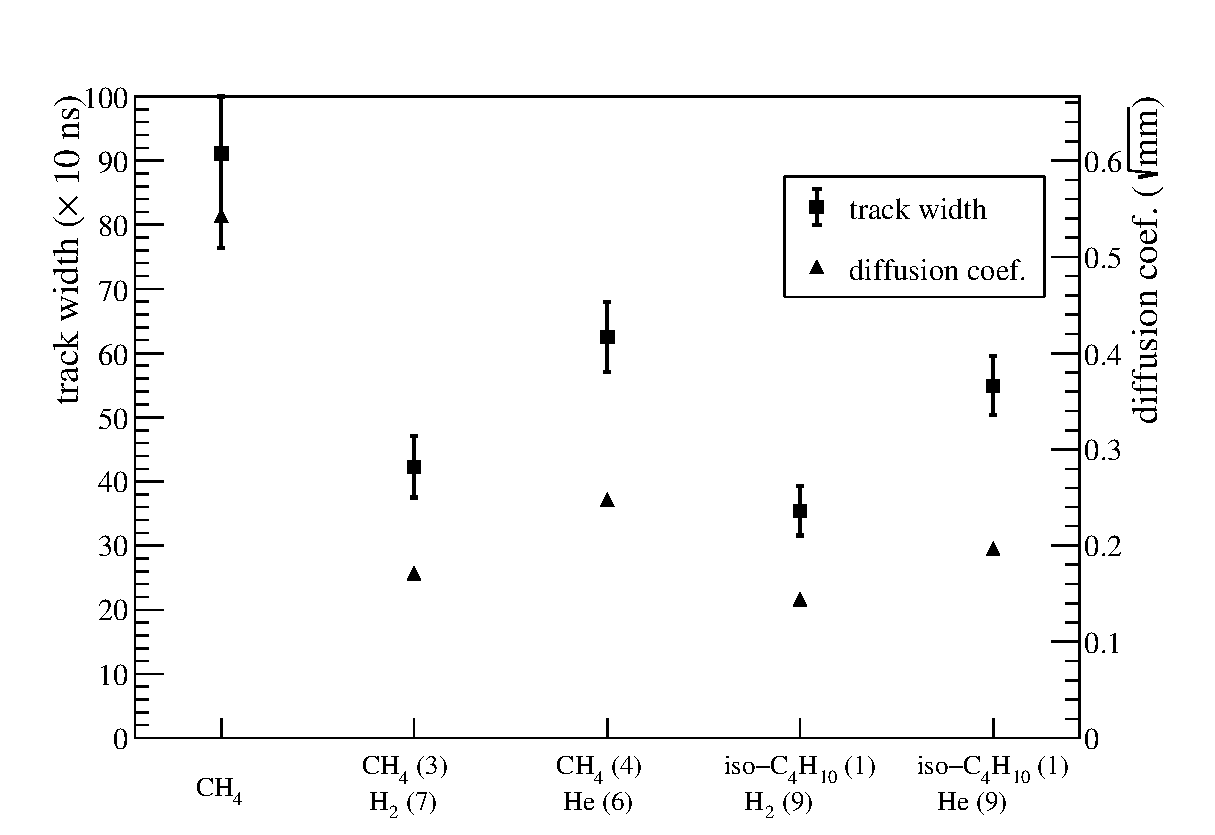
\includegraphics[clip, width=0.9\columnwidth]{diffusion_compare.eps}
  \caption{Magboltz で計算した拡散係数と実測によるトラックの幅.}
  \label{fig::diffusion_compare}
\end{figure}

\section{シミュレーションによる線源データの再現}
MAIKo TPC から得られるトラックをGarfield++~\cite{garfield++}と
Magboltz~\cite{magboltz},SRIM~\cite{SRIM}を用いたシミュレーションによりMAIKo TPC で測定されるトラックの再現を試みた.
シミュレーションでは,ドリフト電場,W値,電子増幅率,検出ガスの密度を固定した上で,
最もよく測定結果を再現する信号の閾値を探索した.
電子増幅率は$\alpha$線源を用いた測定値を用いた.
シミュレーションは以下の手順%(図\ref{fig::simulation_flow})
で行った.
\begin{enumerate}
\item\label{sim::particle_generate}
  トラックを生成する荷電粒子のエネルギー,運動量を決定し,
  Garfield++のSrimTrack に登録する.
\item
  SrimTrack によりトラックの周囲に電子を生成する.
\item
  電子をMagboltz で求めたドリフト速度で読み出し領域へドリフトさせる.
\item
  読み出し領域に到達した電子1つにつき図\ref{fig::mu-pic_readout}に示すような電気信号を
  各strip の信号波形に加算する.
\item
  設定した閾値により,信号波形を白黒画像に変換しanode image とcathode image を生成する.
\end{enumerate}
$\alpha$線源を用いた場合のシミュレーションと測定の比較を図\ref{fig::track_comp_ch4},
\ref{fig::track_comp_ch4_h2}, \ref{fig::track_comp_ch4_he}, 
\ref{fig::track_comp_ic4h10_h2}, \ref{fig::track_comp_ic4h10_he}に示す.
これらの$\alpha$線は図\ref{fig::drift_v_image}のように有感領域を貫通している.
信号の閾値を\SI{0.1}{\milli\volt}とすると,それぞれの検出ガスでの$\alpha$線源によるトラックを,
シミュレーションで再現できる.
\begin{figure}
  \centering
  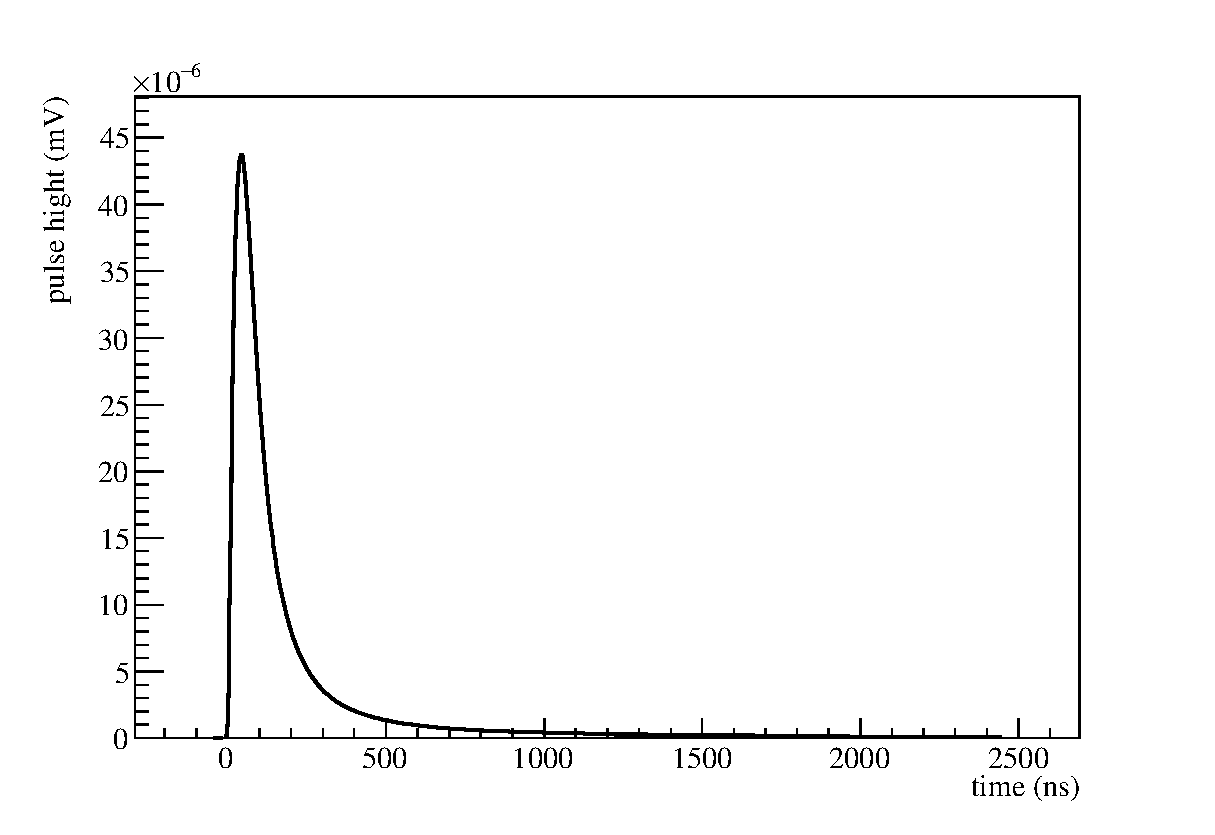
\includegraphics[clip, width=0.9\columnwidth]{waveform.eps}
  \caption{1電子が$\mu$-PICに到達した時に読み出される電気信号.}
  \label{fig::mu-pic_readout}
\end{figure}

\begin{figure}
  \centering
  \begin{subfigure}{0.48\columnwidth}
    \centering
    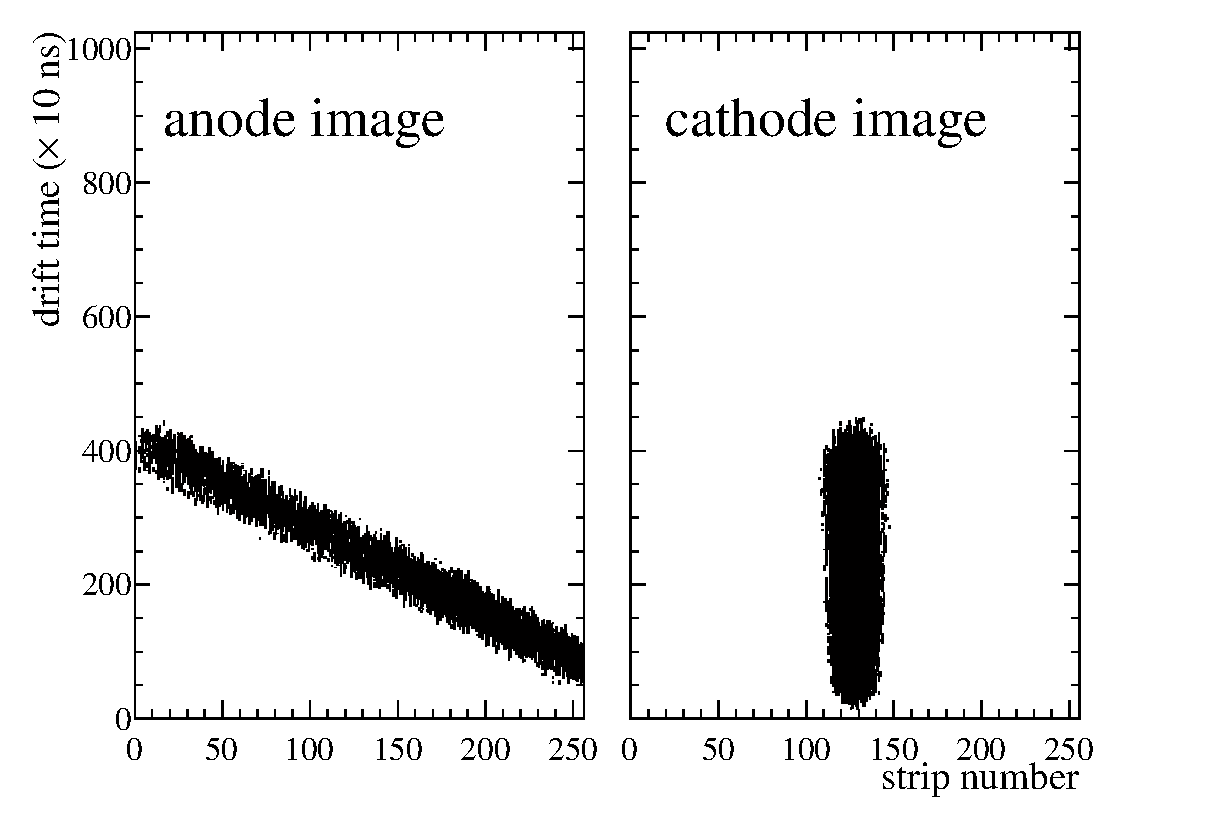
\includegraphics[clip, width=\columnwidth, trim=0 0 50 0]{CH4_0.eps}
    \caption{シミュレーションによるトラック.}
  \end{subfigure}
  \begin{subfigure}{0.48\columnwidth}
    \centering
    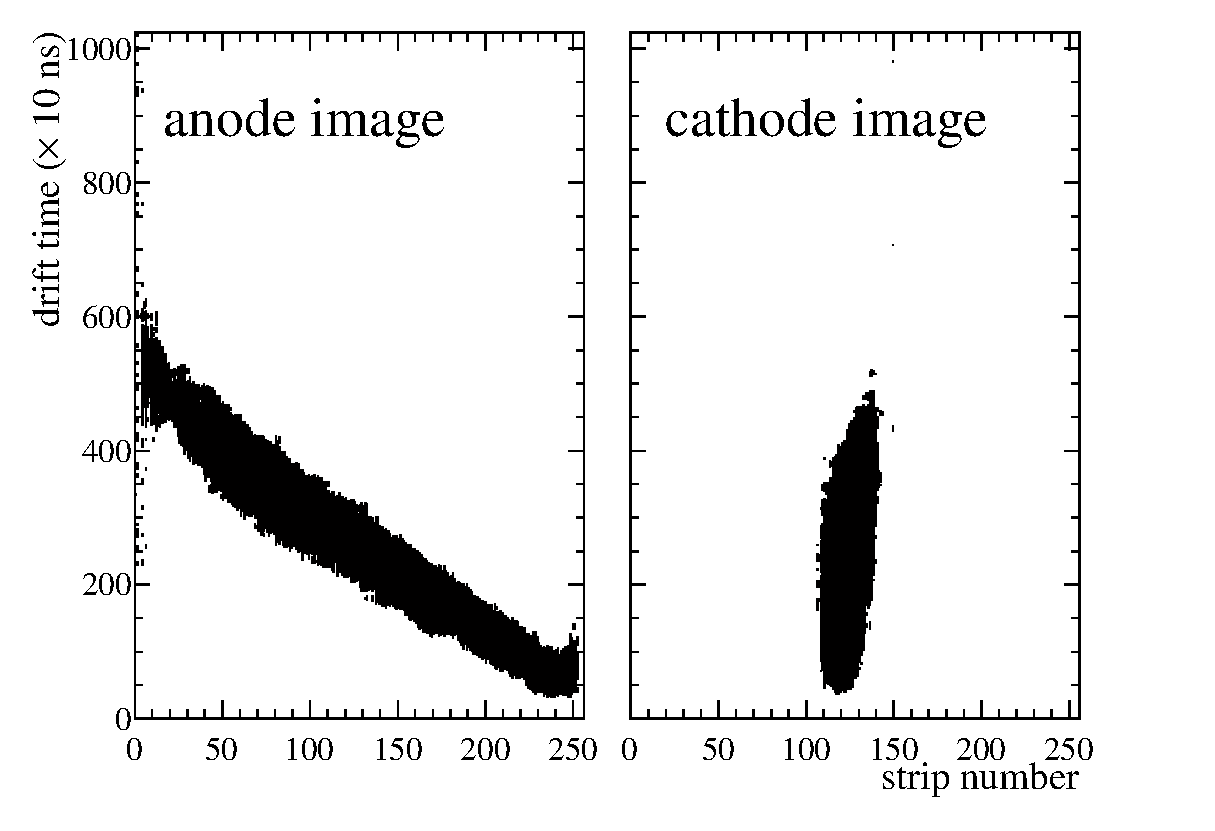
\includegraphics[width=\columnwidth, trim=0 0 50 0]{0160_5.eps}
    \caption{$\alpha$線源によるトラック.}
  \end{subfigure}
  \caption{$\alpha$粒子のトラック(\Methane の場合).}
  \label{fig::track_comp_ch4}
\end{figure}

\begin{figure}
  \centering
  \begin{subfigure}{0.48\columnwidth}
    \centering
    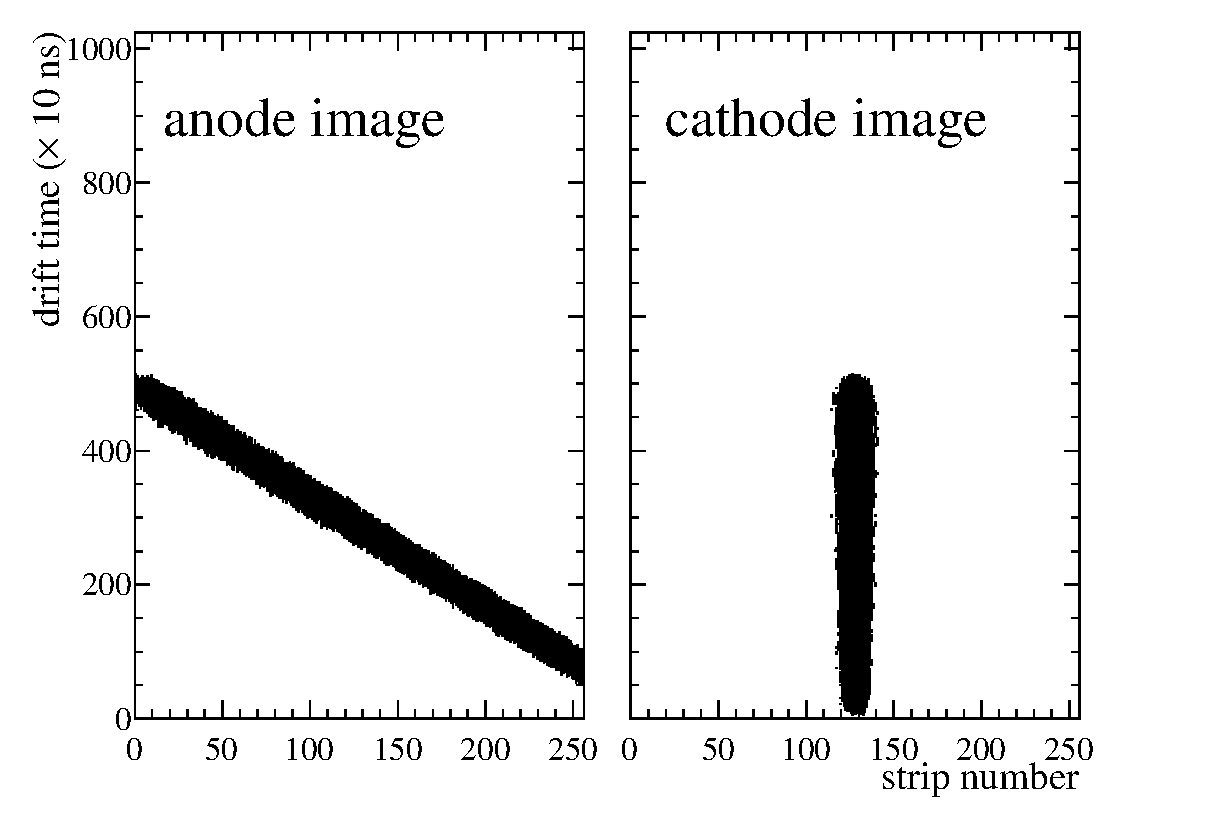
\includegraphics[clip, width=\columnwidth, trim=0 0 50 0]{CH4_3_H2_7_0.eps}
    \caption{シミュレーションによるトラック.}
  \end{subfigure}
  \begin{subfigure}{0.48\columnwidth}
    \centering
    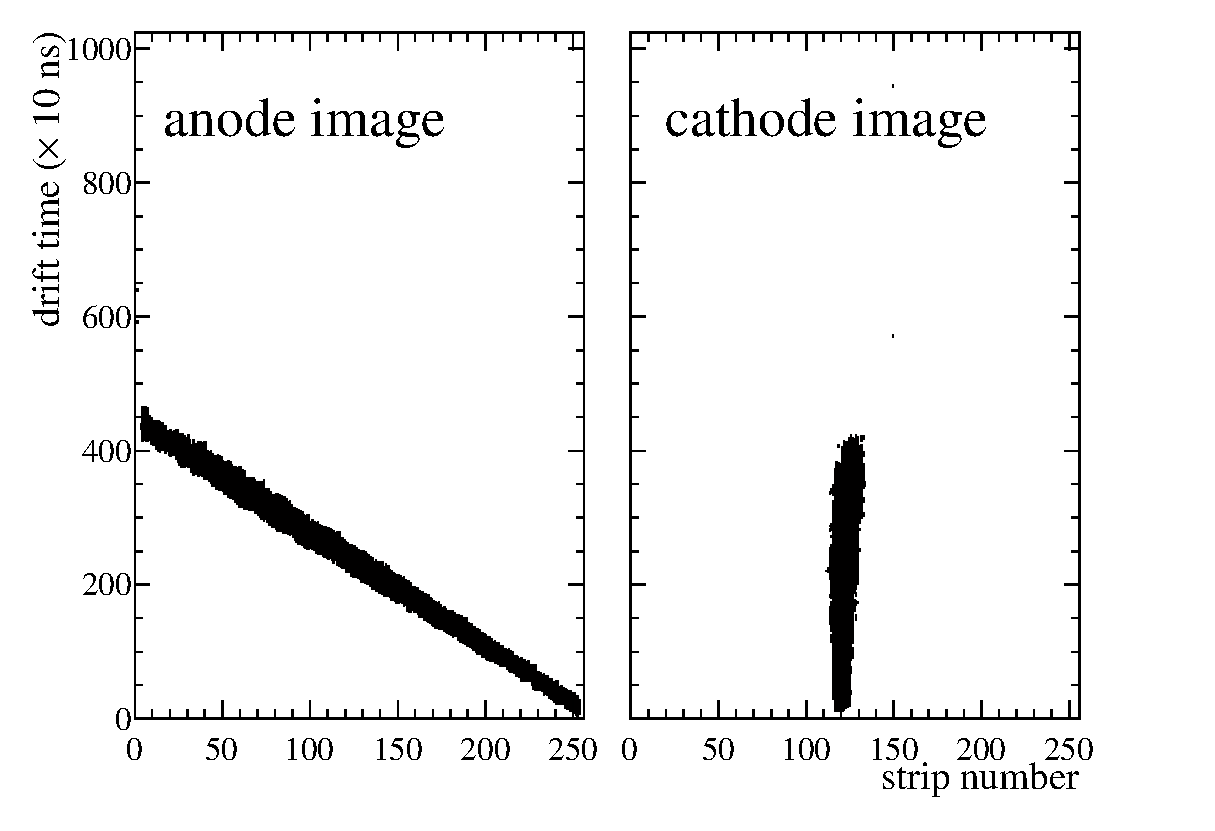
\includegraphics[clip, width=\columnwidth, trim=0 0 50 0]{0207_7.eps}
    \caption{$\alpha$線源によるトラック.}
  \end{subfigure}
  \caption{$\alpha$粒子のトラック(\MethaneHydro の場合).}
  \label{fig::track_comp_ch4_h2}
\end{figure}

\begin{figure}
  \centering
  \begin{subfigure}{0.48\columnwidth}
    \centering
    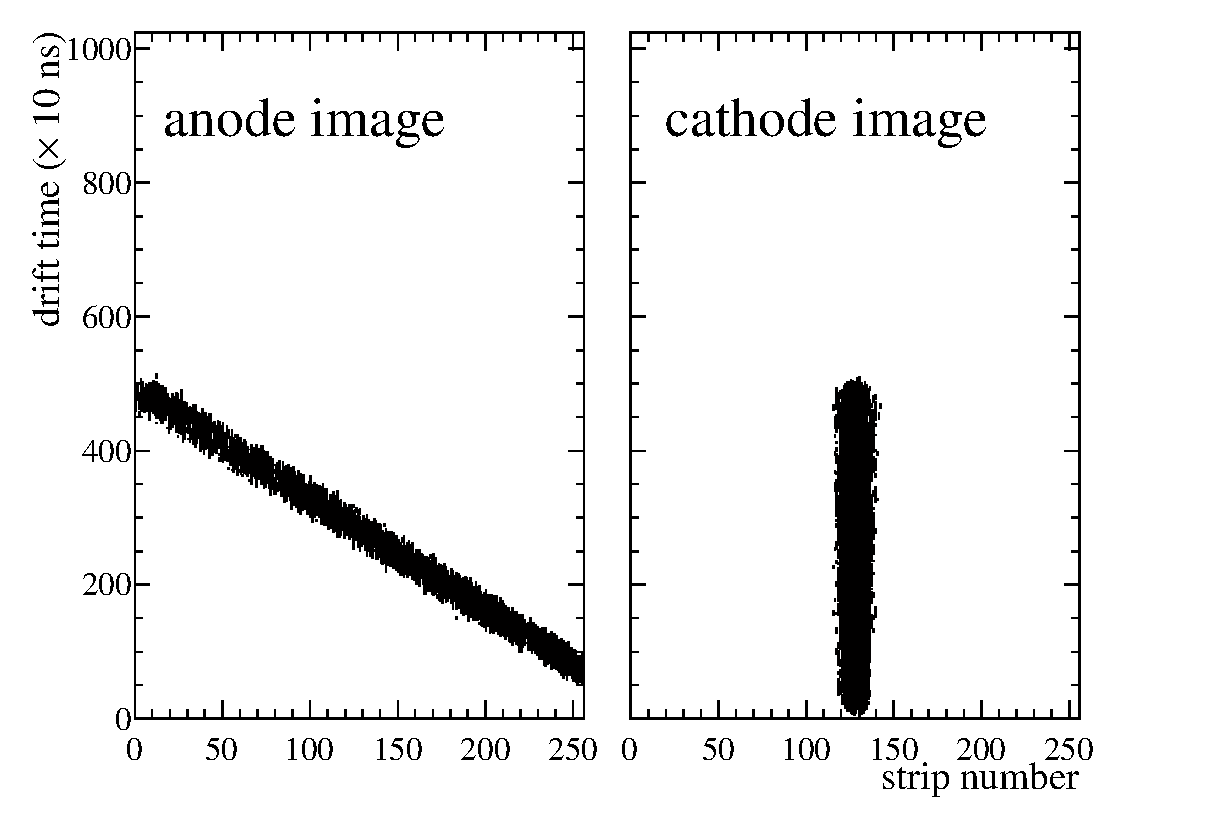
\includegraphics[clip, width=\columnwidth, trim=0 0 50 0]{CH4_4_He_6_0.eps}
    \caption{シミュレーションによるトラック.}
  \end{subfigure}
  \begin{subfigure}{0.48\columnwidth}
    \centering
    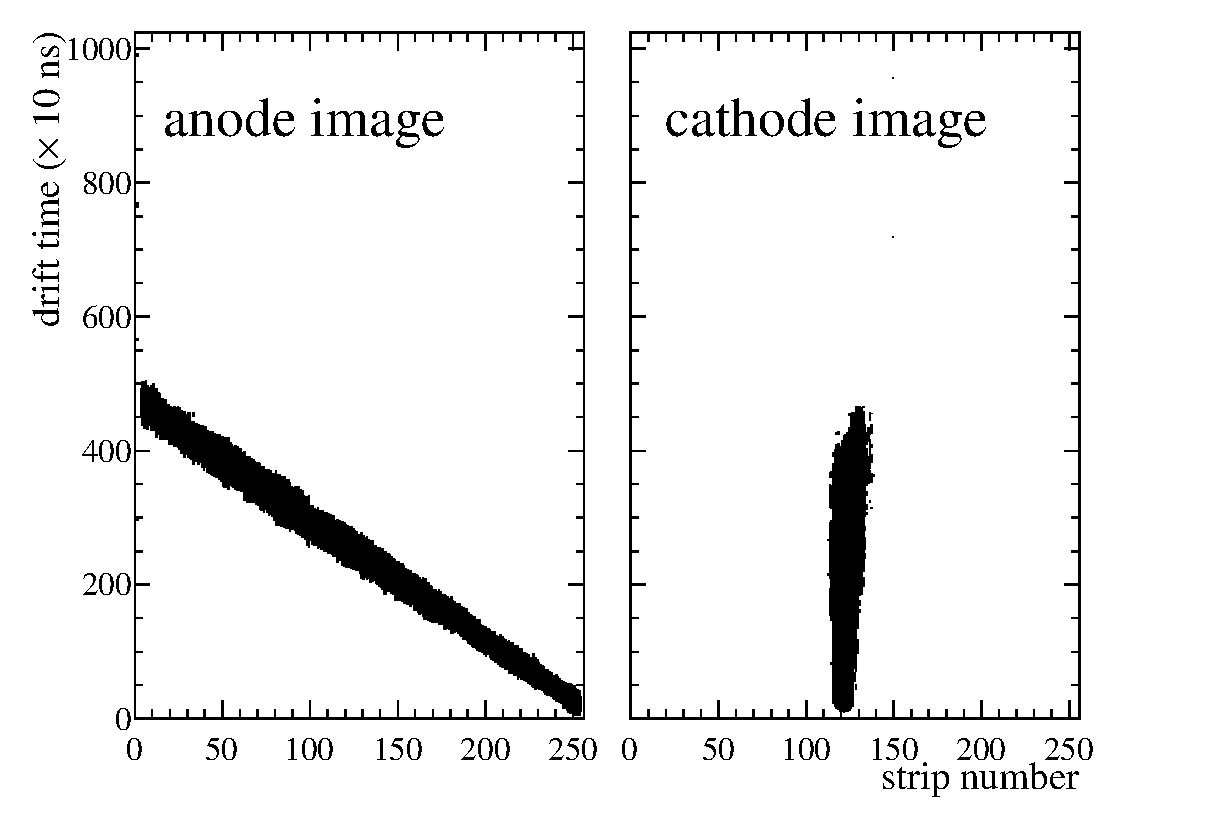
\includegraphics[clip, width=\columnwidth, trim=0 0 50 0]{0163_3.eps}
    \caption{$\alpha$線源によるトラック.}
  \end{subfigure}
  \caption{$\alpha$粒子のトラック [\MethaneHerium の場合].}
  \label{fig::track_comp_ch4_he}
\end{figure}

\begin{figure}
  \centering
  \begin{subfigure}{0.48\columnwidth}
    \centering
    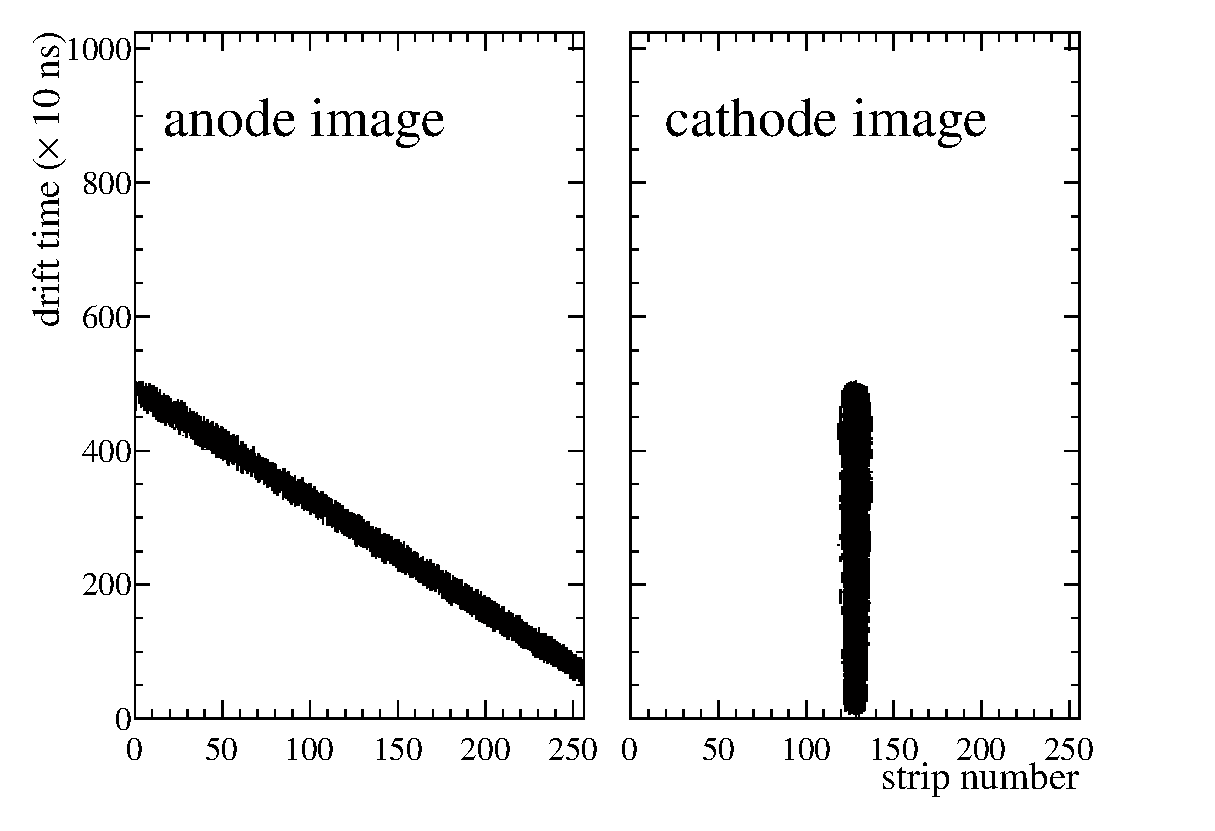
\includegraphics[clip, width=\columnwidth, trim=0 0 50 0]{iC4H10_1_H2_9_0.eps}
    \caption{シミュレーションによるトラック.}
  \end{subfigure}
  \begin{subfigure}{0.48\columnwidth}
    \centering
    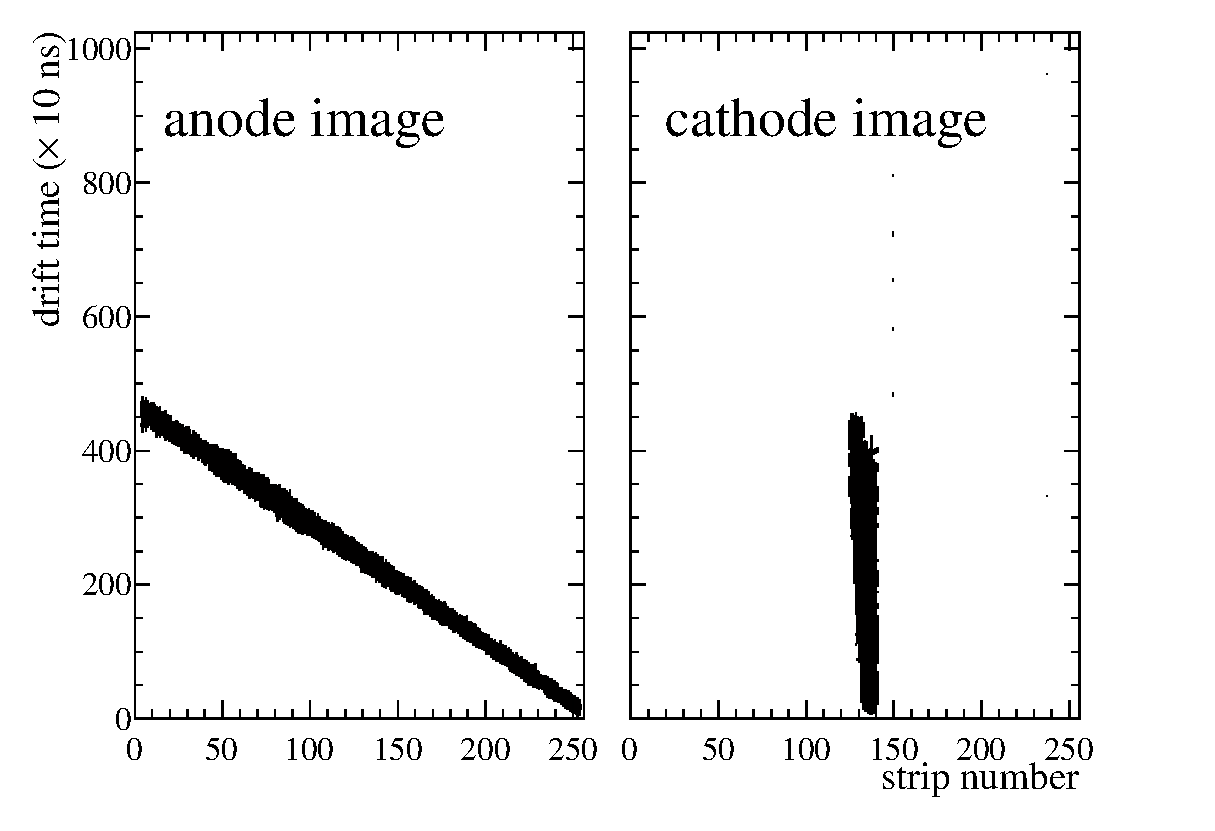
\includegraphics[clip, width=\columnwidth, trim=0 0 50 0]{0210_14.eps}
    \caption{$\alpha$線源によるトラック.}
  \end{subfigure}
  \caption{$\alpha$粒子のトラック [\isoButaneHydro の場合].}
  \label{fig::track_comp_ic4h10_h2}
\end{figure}

\begin{figure}
  \centering
  \begin{subfigure}{0.48\columnwidth}
    \centering
    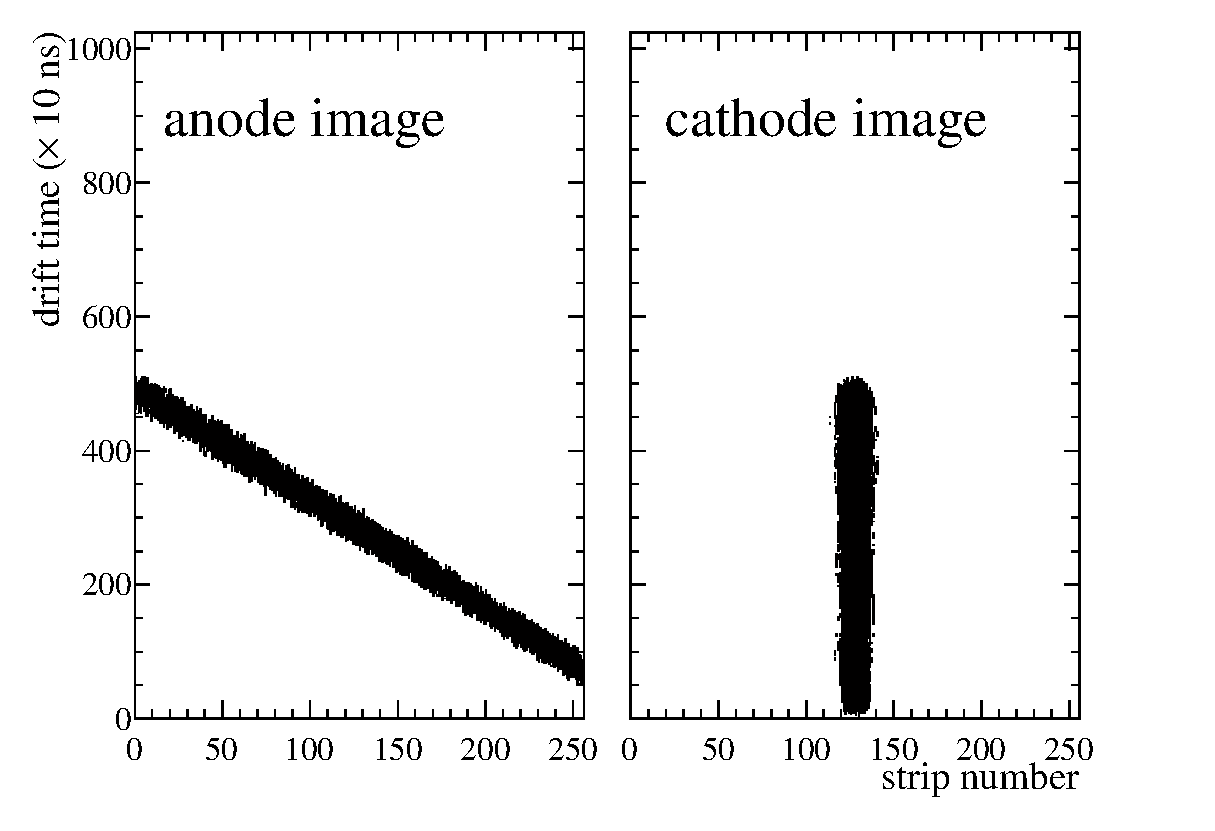
\includegraphics[clip, width=\columnwidth, trim=0 0 50 0]{iC4H10_1_He_9_0.eps}
    \caption{シミュレーションによるトラック.}
  \end{subfigure}
  \begin{subfigure}{0.48\columnwidth}
    \centering
    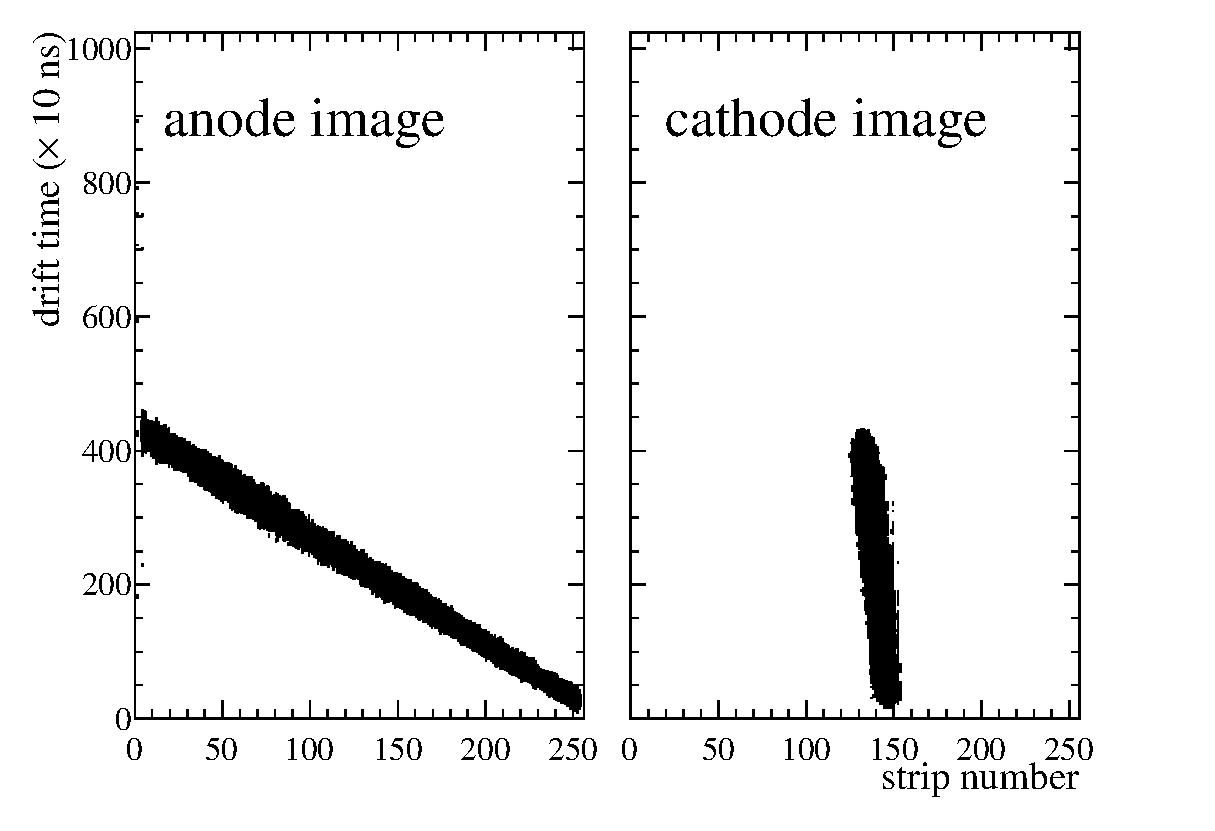
\includegraphics[clip, width=\columnwidth, trim=0 0 50 0]{0176_1.eps}
    \caption{$\alpha$線源によるトラック.}
  \end{subfigure}
  \caption{$\alpha$粒子のトラック [\isoButaneHerium の場合].}
  \label{fig::track_comp_ic4h10_he}
\end{figure}

$\alpha$線源から放出される$\alpha$粒子のエネルギーは平均\SI{4.2}{\mega\electronvolt}である.
一方で,本研究の目的である$0_2^+$状態からの崩壊$\alpha$粒子のエネルギーは数百\si{\kilo\electronvolt}である.
そこで,$\alpha$線源の前に\SI{15}{\micro\metre}のカプトンを設置することで
低エネルギー$\alpha$粒子での測定を行った.
$\alpha$粒子のエネルギーは有感領域と線源の間にある検出ガスによってさらに低下し約\SI{1}{\mega\electronvolt}となる.
図\ref{fig::track_ch4_loss},\ref{fig::track_ch4_h2_loss},\ref{fig::track_ch4_he_loss},
\ref{fig::track_ic4h10_h2_loss},\ref{fig::track_ic4h10_he_loss}に示す.
コリメータの\ang{30}の穴を用いたため,斜めのトラックとなっている.
シミュレーションでは有感領域の横から\SI{500}{\kilo\electronvolt}の$\alpha$粒子を入射させた.
これらの$\alpha$粒子はMAIKo TPC の有感領域中で停止している.
$\alpha$線源から放出されるエネルギーに広がりがあるため,
エネルギーを完全に一致できていないが,トラックの傾向は再現できている.
\begin{figure}
  \centering
  \begin{subfigure}{0.48\columnwidth}
    \centering
    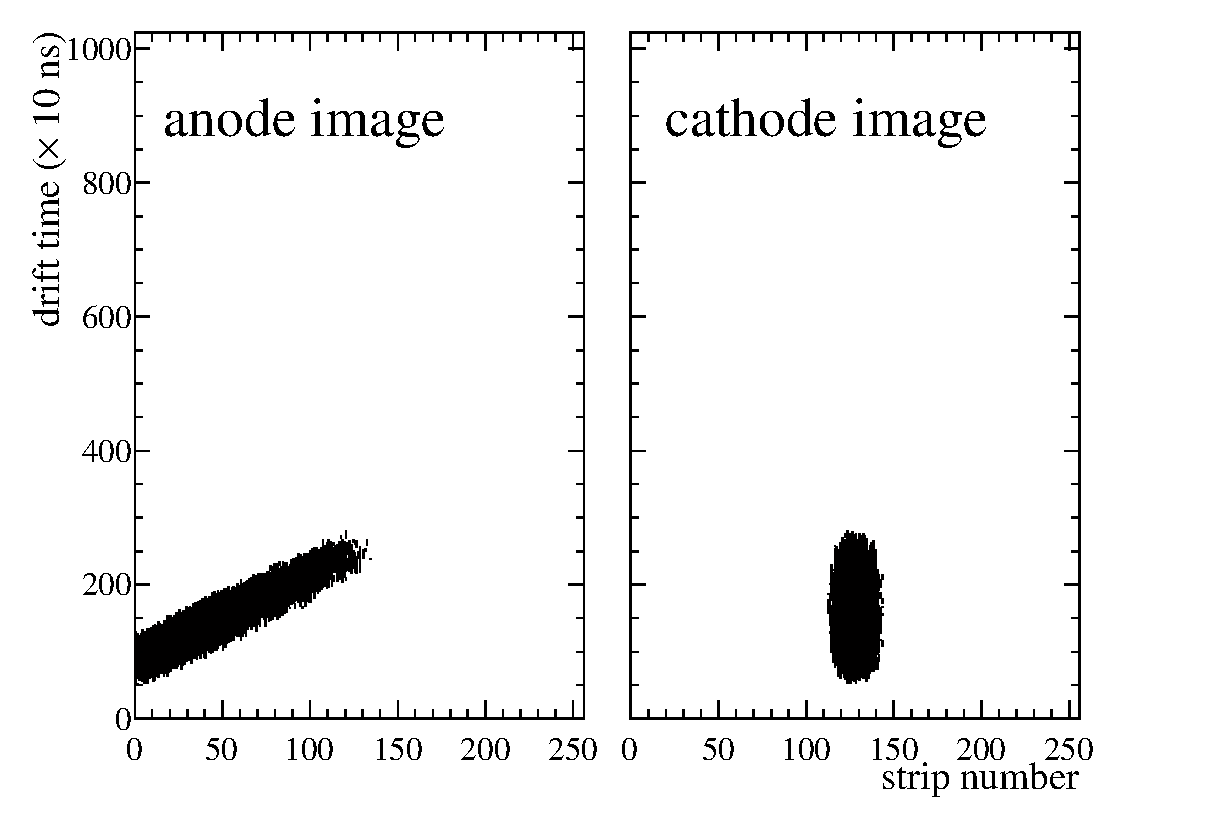
\includegraphics[clip, width=\columnwidth, trim=0 0 50 0]{a_source_CH4_50_nostr_3.eps}
    \caption{シミュレーションによるトラック.}
  \end{subfigure}
  \begin{subfigure}{0.48\columnwidth}
    \centering
    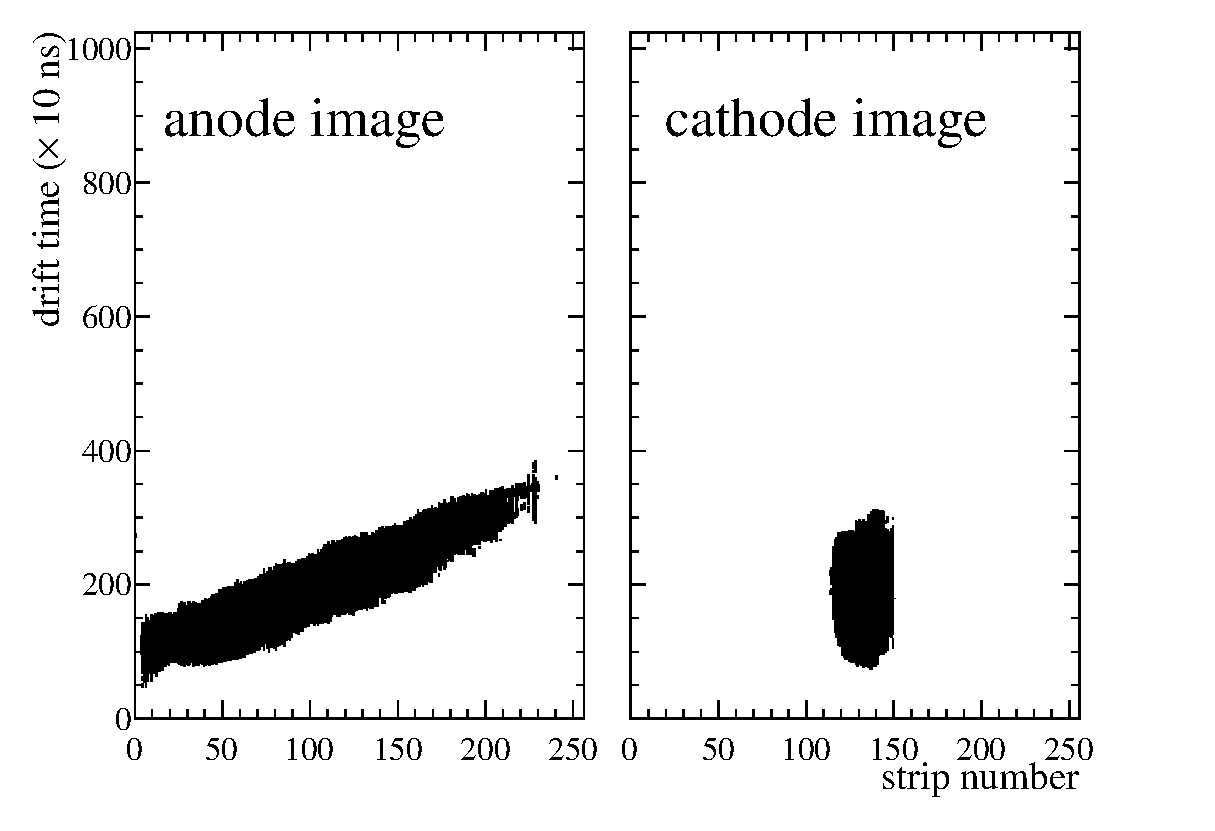
\includegraphics[clip, width=\columnwidth, trim=0 0 50 0]{0146_16.eps}
    \caption{$\alpha$線源によるトラック.}
  \end{subfigure}
  \caption{低エネルギー$\alpha$粒子のトラック [\Methane の場合].}
  \label{fig::track_ch4_loss}
\end{figure}
\begin{figure}
  \centering
  \begin{subfigure}{0.48\columnwidth}
    \centering
    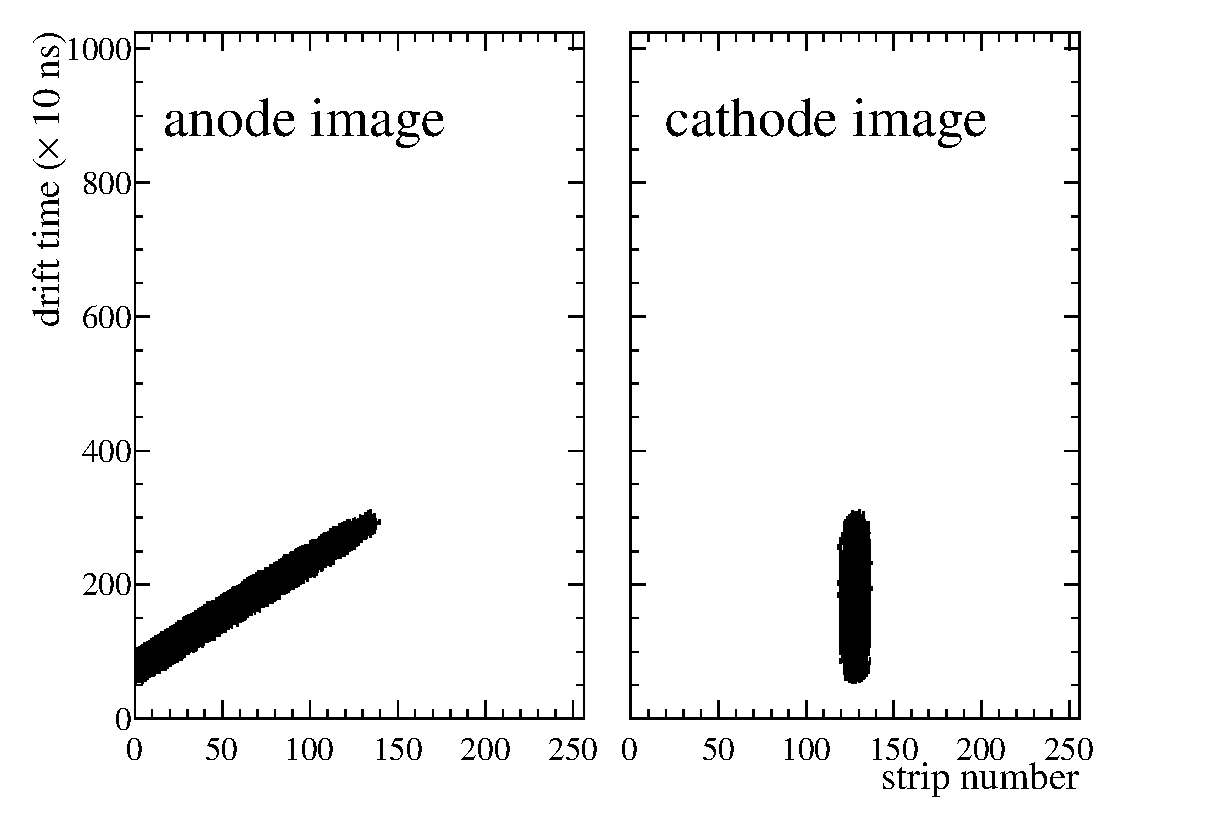
\includegraphics[clip, width=\columnwidth, trim=0 0 50 0]{a_source_CH4_3_H2_7_100_nostr_0.eps}
    \caption{シミュレーションによるトラック.}
  \end{subfigure}
  \begin{subfigure}{0.48\columnwidth}
    \centering
    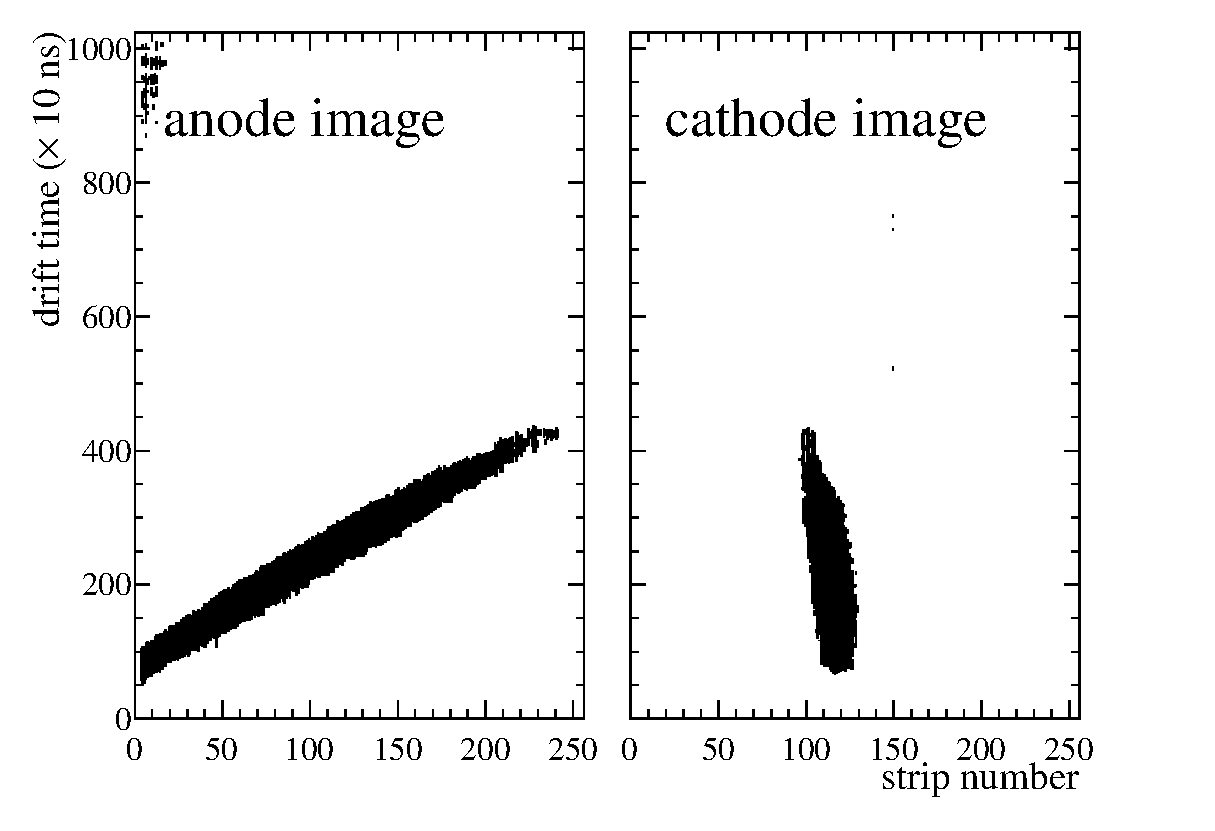
\includegraphics[clip, width=\columnwidth, trim=0 0 50 0]{0209_22.eps}
    \caption{$\alpha$線源によるトラック.}
  \end{subfigure}
  \caption{低エネルギー$\alpha$粒子のトラック [\MethaneHydro の場合].}
  \label{fig::track_ch4_h2_loss}
\end{figure}
\begin{figure}
  \centering
  \begin{subfigure}{0.48\columnwidth}
    \centering
    \includegraphics[clip, width=\columnwidth, trim=0 0 50 0]{a_source_CH4_4_He_6_100_nostr_0.eps}
    \caption{シミュレーションによるトラック.}
  \end{subfigure}
  \begin{subfigure}{0.48\columnwidth}
    \centering
    \includegraphics[clip, width=\columnwidth, trim=0 0 50 0]{0204_24.eps}
    \caption{$\alpha$線源によるトラック.}
  \end{subfigure}
  \caption{低エネルギー$\alpha$粒子のトラック [\MethaneHerium の場合].}
  \label{fig::track_ch4_he_loss}
\end{figure}
\begin{figure}
  \centering
  \begin{subfigure}{0.48\columnwidth}
    \centering
    \includegraphics[clip ,width=\columnwidth, trim=0 0 50 0]{a_source_iC4H10_1_H2_9_100_nostr_1.eps}
    \caption{シミュレーションによるトラック.}
  \end{subfigure}
  \begin{subfigure}{0.48\columnwidth}
    \centering
    \includegraphics[clip, width=\columnwidth, trim=0 0 50 0]{0211_4.eps}
    \caption{$\alpha$線源によるトラック.}
  \end{subfigure}
  \caption{低エネルギー$\alpha$粒子のトラック [\isoButaneHydro の場合].}
  \label{fig::track_ic4h10_h2_loss}
\end{figure}
\begin{figure}
  \centering
  \begin{subfigure}{0.48\columnwidth}
    \centering
    \includegraphics[clip, width=\columnwidth, trim=0 0 50 0]{a_source_iC4H10_1_He_9_100_nostr_0.eps}
    \caption{シミュレーションによるトラック.}
  \end{subfigure}
  \begin{subfigure}{0.48\columnwidth}
    \centering
    \includegraphics[clip, width=\columnwidth, trim=0 0 50 0]{0203_10.eps}
    \caption{$\alpha$線源によるトラック.}
  \end{subfigure}
  \caption{低エネルギー$\alpha$粒子のトラック [\isoButaneHerium の場合].}
  \label{fig::track_ic4h10_he_loss}
\end{figure}

\section{トリプルアルファ反応のシミュレーション}
\label{sec::triple_alpha_simulation}
$\alpha$線源から放出される$\alpha$粒子のトラックを再現することができたので,
同じ設定で${}^{12}{\mathrm{C}}({\mathrm{n}},{\mathrm{n}}')3\alpha$のシミュレーションを行った.
このシミュレーションでは以下のように3つの$\alpha$粒子を生成した.
\begin{enumerate}
\item
  ${}^{12}\mathrm{C}$を\SI{14}{\mega\electronvolt}の中性子との散乱により$0_2^+$状態に励起させる.
  この際,重心系で一様な散乱角で散乱させる.
\item
  ${}^{12}\mathrm{C} (0_2^+)$を$\alpha$粒子と${}^{8}\mathrm{Be}$に位相空間で一様に崩壊させる.
\item
  崩壊してできた${}^{8}\mathrm{Be}$を2つの$\alpha$粒子へ位相空間で一様に崩壊させる.
\end{enumerate}
このようにして得た$\alpha$粒子のトラックを生成する.
トラックの生成方法は前節で述べた通りである.
生成したトラックを図\ref{fig::three_alpha_ch4}, \ref{fig::three_alpha_ch4_h2}, \ref{fig::three_alpha_ch4_he},
\ref{fig::three_alpha_ic4h10_h2}, \ref{fig::three_alpha_ic4h10_he}に示す.
ここでは,3つのトラックを確認できたイベントを示した.
生成されたイベントの中には$\alpha$粒子のエネルギーと放出角度によっては,
3本のトラックを確認できないイベントも含まれている.
図\ref{fig::not_three_alpha_ch4},\ref{fig::not_three_alpha_ch4_h2},\ref{fig::not_three_alpha_ch4_he},
\ref{fig::not_three_alpha_ic4h10_h2},\ref{fig::not_three_alpha_ic4h10_he}に2本しかトラックを確認できないイベントを示す.

\begin{figure}
  \centering
  \includegraphics[clip, width=0.8\columnwidth]{10020_7.eps}
  \caption{3$\alpha$のシミュレーション画像 [\Methane の場合].}
  \label{fig::three_alpha_ch4}
\end{figure}

\begin{figure}
  \centering
  \includegraphics[clip, width=0.8\columnwidth]{10022_15.eps}
  \caption{3$\alpha$のシミュレーション画像 [\MethaneHydro の場合].}
  \label{fig::three_alpha_ch4_h2}
\end{figure}

\begin{figure}
  \centering
  \includegraphics[clip, width=0.8\columnwidth]{10021_5.eps}
  \caption{3$\alpha$のシミュレーション画像 [\MethaneHerium の場合].}
  \label{fig::three_alpha_ch4_he}
\end{figure}

\begin{figure}
  \centering
  \includegraphics[clip, width=0.8\columnwidth]{10024_9.eps}
  \caption{3$\alpha$のシミュレーション画像 [\isoButaneHydro の場合].}
  \label{fig::three_alpha_ic4h10_h2}
\end{figure}

\begin{figure}
  \centering
  \includegraphics[clip, width=0.8\columnwidth]{10023_0.eps}
  \caption{3$\alpha$のシミュレーション画像 [\isoButaneHerium の場合].}
  \label{fig::three_alpha_ic4h10_he}
\end{figure}
\begin{figure}
  \centering
  \includegraphics[clip, width=0.8\columnwidth]{10020_5.eps}
  \caption{2本しかトラックを確認できないイベントの画像 [\Methane の場合].}
  \label{fig::not_three_alpha_ch4}
\end{figure}
\begin{figure}
  \centering
  \includegraphics[clip, width=0.8\columnwidth]{10022_49.eps}
  \caption{2本しかトラックを確認できないイベントの画像 [\MethaneHydro の場合].}
  \label{fig::not_three_alpha_ch4_h2}
\end{figure}
\begin{figure}
  \centering
  \includegraphics[clip, width=0.8\columnwidth]{10021_24.eps}
  \caption{2本しかトラックを確認できないイベントの画像 [\MethaneHerium の場合].}
  \label{fig::not_three_alpha_ch4_he}
\end{figure}
\begin{figure}
  \centering
  \includegraphics[clip, width=0.8\columnwidth]{10024_25.eps}
  \caption{2本しかトラックを確認できないイベントの画像 [\isoButaneHydro の場合].}
  \label{fig::not_three_alpha_ic4h10_h2}
\end{figure}
\begin{figure}
  \centering
  \includegraphics[clip, width=0.8\columnwidth]{10023_32.eps}
  \caption{2本しかトラックを確認できないイベントの画像 [\isoButaneHerium の場合].}
  \label{fig::not_three_alpha_ic4h10_he}
\end{figure}

\end{document}

\documentclass[../master]{subfiles}

\begin{document}

\chapter{解析}
%\section{液体シンチレータの解析}
%\subsection{FADCの生データ}
%光電子増倍管から取得した波形データの一例を示す.
%
%\subsection{波形弁別 (n-$\gamma$ discrimination)}
%液体シンチレータのデータの中には中性子による信号とガンマ線による信号とが含まれている.
%この2つの波形には違いがあるので,その波形の違いから識別することができる.
%
%\subsection{中性子のレート}
%中性子線源から放出される中性子の量は時間とともに変化する.
%
\section{解析の概要}
MAIKo TCP の解析では背景事象の除去とトラック情報の抽出の2つが必要となる.
検出ガスには${}^{12}\mathrm{C}$だけでなく,陽子や${}^{4}\mathrm{He}$が含まれる.
そのため,中性子と陽子,${}^{4}\mathrm{He}$との散乱事象を取り除く必要がある.
その後,中性子と${}^{12}\mathrm{C}$との散乱事象に対してトラックの情報を抽出する.
トラックの情報は中性子と${}^{12}\mathrm{C}$とが散乱した座標,
$\alpha$粒子が停止した座標である.
anode image から$z, y$座標を,cathode image から$x, y$座標を決定することができる.
$x, z$座標は$\mu$-PIC の信号を検出したstrip のチャンネル番号に\SI{400}{\micro\metre}をかけることで求めることができる.
TPC では,$y$座標を荷電粒子が通過した位置から読み出し面に到達するまでの時間として測定する.
そのため,anode image, cathode image のclock にドリフトスピードをかけることで$y$座標を求めることができる.
このようにして決定したanode image, cathode image の座標を合わせることで,
3次元の座標を求めることができる.

散乱点と停止点の座標から粒子が飛行した方向ベクトルと距離が決定される.
粒子が分かれば,飛行距離から運動エネルギーが決まる.
図\ref{fig::range_to_ene_alpha}に\Methane (\SI{50}{\hecto\pascal}) 中での荷電粒子の飛行距離と運動エネルギーの対応を示す.
飛行距離と運動エネルギーの相関はSRIM~\cite{SRIM}を用いて求めた.
SRIM は,荷電粒子がが物質中を通過する際の,イオンの飛程,エネルギーロス等を算出するシミュレーションソフトウェアである.
この対応関係から粒子の運動エネルギーを決定する.
粒子の運動エネルギーを$T$,質量を$m$,単位方向ベクトルを$(dx, dy, dz)$とすると,
粒子の4元運動量は
\begin{equation}
  p =
  \begin{pmatrix}
    E \\ p_{x} \\ p_{y} \\ p_{z}
  \end{pmatrix}
  =
  \begin{pmatrix}
    T + m \\ \sqrt{(T+m)^2 + m^2} dx \\ \sqrt{(T+m)^2 + m^2} dy \\ \sqrt{(T+m)^2 + m^2} dz
  \end{pmatrix}
  \label{eq::momentum_vector}
\end{equation}
となる.
決定した3つの$\alpha$粒子の4元運動量を足し合わせることで,${}^{12}\mathrm{C}$の4元運動量を再構成できる.
このようにして求めた4元運動量から,
${}^{12}\mathrm{C}$の運動エネルギー,散乱角度,励起エネルギーを求めることができる.
\begin{figure}
  \centering
  \includegraphics[clip, width=0.8\columnwidth]{range_to_ene.eps}
  \caption[\Methane (\SI{50}{\hecto\pascal}) 中での荷電粒子 (p, $\alpha$, ${}^{12}\rm{C}$) の飛行距離と運動エネルギー.]
          {\Methane (\SI{50}{\hecto\pascal}) 中での荷電粒子 (p, $\alpha$, ${}^{12}\rm{C}$) の飛行距離と運動エネルギー.
            この相関はSRIM を用いて求めた.
          }
  \label{fig::range_to_ene_alpha}
\end{figure}

%\subsection{機械学習}
%これまではHough 変換を使って解析を行ってきたが,
%高速に処理をするためにニューラルネットワークを用いた解析方法を開発した.

\section{eye-scan}
本研究ではMAIKo TPC から得られたトラックの解析を人間の目 (eye-scan) で行った.
eye-scanでは,トラックの本数の識別と散乱点,停止点の抽出を行った.
ここではトラックの本数が3本であるイベントを${}^{12}\mathrm{C}(\mathrm{n},\mathrm{n}')3\alpha$イベントとした.
本研究では${}^{12}\mathrm{C}(\mathrm{n},\mathrm{n}')3\alpha$イベントに対して解析を行った.
検出ガスの決定のために,\ref{sec::triple_alpha_simulation}節のシミュレーションで生成したデータのうち,
有感領域中で3つの$\alpha$粒子が停止したイベントに対して解析を行った.

\subsection{解析効率}
実際には${}^{12}\mathrm{C}(\mathrm{n},\mathrm{n}')3\alpha$イベントであっても,
各$\alpha$粒子のエネルギーや放出角度,トラックの太さによっては3つのトラックを区別することができず,
${}^{12}\mathrm{C}(\mathrm{n},\mathrm{n}')3\alpha$イベントとして認識できない場合がある.
そこで,eye-scanによって正しくトラックが3本と認識できる割合(解析効率)を評価する.
eye-scanは各検出ガスについて100 events ずつ行った.
eye-scanによって決定したトラックの本数を表\ref{tab::track_number_ratio}に示す.
表\ref{tab::track_number_ratio}の3本の割合が解析効率となる.
\Methane 単体と\MethaneHerium 以外は約\SI{90}{\percent}の解析効率となっている.
%\begin{table}
%  \centering
%  \caption[シミュレーションデータに対する検出効率.]
%          {シミュレーションデータに対する検出効率.
%            検出効率は全イベントに対して3本のトラックをすべて認識できた割合である.}
%  \label{tab::detection_efficiency}
%  \begin{tabular}{cc}
%    \toprule
%    gas & 検出効率 (\%)\\
%    \midrule
%    \Methane & $55$ \\% \pm 7.42$ \\
%    \MethaneHydro & $91$ \\% \pm 9.54$ \\
%    \MethaneHerium & $78$ \\% \pm 8.83$ \\
%    \isoButaneHydro & $87$ \\% \pm 9.33$ \\
%    \isoButaneHerium & $90$ \\% \pm 9.49$ \\
%    \bottomrule
%  \end{tabular}
%\end{table}
\begin{table}
  \centering
  \caption{eye-scanによって決定したトラックの本数の割合.}
  \label{tab::track_number_ratio}
  \begin{tabular}{cccc}
    \toprule
    gas & 3本 (\si{\percent}) & 2本 (\si{\percent}) & 1本 (\si{\percent}) \\
    \midrule
    \Methane & 55 & 37 & 8 \\
    \MethaneHydro & 91 & 9 & 0 \\
    \MethaneHerium & 78 & 22 & 0 \\
    \isoButaneHydro & 87 & 11 & 2 \\
    \isoButaneHerium & 90 & 10 & 0 \\
    \bottomrule
  \end{tabular}
\end{table}

%\subsection{検出効率の角度依存性}
\subsection{エネルギー分解能}
$\alpha$粒子の飛行距離の分解能により,エネルギー分解能が決まる.
そこで,eye-scanによる$\alpha$粒子のエネルギー分解能を評価する.
シミュレーションで粒子を生成した時に決定した$\alpha$粒子の運動エネルギー ($E_{\text{ideal}}$) と
eye-scanによって決定した$\alpha$粒子の運動エネルギー ($E_{\text{eye-scan}}$) の相関を
図\ref{fig::E_corr_ch4}, \ref{fig::E_corr_ch4_h2}, \ref{fig::E_corr_ch4_he},
\ref{fig::E_corr_ic4h10_h2}, \ref{fig::E_corr_ic4h10_he}に示す.
縦軸がシミュレーションで決定した運動エネルギー,横軸がeye-scanで決定した運動エネルギーである.
この相関に対して1次関数 ($E_{\text{ideal}} = p_0\times E_{\text{eye-scan}}+p_1$) でフィットした結果を
表\ref{tab::E_corr_params}にまとめる.
どの検出ガスについても,ほぼ$E_{\text{ideal}} = E_{\text{eye-scan}}$となっている.
\begin{figure}
  \centering
  \begin{minipage}{0.45\columnwidth}
    \centering
    \includegraphics[clip, width=\columnwidth]{E_corr_10020.eps}
    \caption{\Methane の場合の$E_{\text{eye-scan}}$と$E_{\text{ideal}}$の相関.}
    \label{fig::E_corr_ch4}
  \end{minipage}  
\end{figure}
\begin{figure}
  \centering
  \begin{minipage}{0.45\columnwidth}
    \centering
    \includegraphics[clip, width=\columnwidth]{E_corr_10022.eps}
    \caption{\MethaneHydro の場合の$E_{\text{eye-scan}}$と$E_{\text{ideal}}$の相関.}
    \label{fig::E_corr_ch4_h2}
  \end{minipage}
  \begin{minipage}{0.45\columnwidth}
    \centering
    \includegraphics[clip, width=\columnwidth]{E_corr_10021.eps}
    \caption{\MethaneHerium の場合の$E_{\text{eye-scan}}$と$E_{\text{ideal}}$の相関.}
    \label{fig::E_corr_ch4_he}
  \end{minipage}
\end{figure}
\begin{figure}
  \centering
  \begin{minipage}{0.45\columnwidth}
    \centering
    \includegraphics[clip, width=\columnwidth]{E_corr_10024.eps}
    \caption{\isoButaneHydro の場合の$E_{\text{eye-scan}}$と$E_{\text{ideal}}$の相関.}
    \label{fig::E_corr_ic4h10_h2}
  \end{minipage}
  \begin{minipage}{0.45\columnwidth}
    \centering
    \includegraphics[clip, width=\columnwidth]{E_corr_10023.eps}
    \caption{\isoButaneHerium の場合の$E_{\text{eye-scan}}$と$E_{\text{ideal}}$の相関.}
    \label{fig::E_corr_ic4h10_he}
  \end{minipage}
\end{figure}
\begin{table}
  \centering
  \caption{}
  \label{tab::E_corr_params}
  \begin{tabular}{ccc}
    \toprule
    gas & $p_0$ & $p_1$ \\
    \midrule
    \Methane  & 0.985 & 0.0179 \\
    \MethaneHydro & 0.991 & 0.00260 \\
    \MethaneHerium  & 0.972 & 0.0157 \\
    \isoButaneHydro & 0.929 & 0.0309 \\
    \isoButaneHerium  & 0.962 & 0.0166 \\
    \bottomrule
  \end{tabular}
\end{table}

$E_{\text{eye-scan}}$をフィットした1次関数 ($f(x)$) で補正したエネルギーと$E_{\text{ideal}}$と
差分を$dE\ (=E_{\text{ideal}}-f(E_{\text{eye-scan}}))$とする.
各検出ガスでの$dE$の分布を図\ref{fig::dE_ch4}, \ref{fig::dE_ch4_h2}, \ref{fig::dE_ch4_he},
\ref{fig::dE_ic4h10_h2}, \ref{fig::dE_ic4h10_he}に,ガウス分布でフィットした中心値と分散を表\ref{tab::gas_summary}に示す.
エネルギー分解能は,\MethaneHydro の場合に最も小さいことが分かる.
%混合ガスの場合,分散は約20 keV となっている.
\begin{figure}
  \centering
  \begin{minipage}{0.45\columnwidth}
    \centering
    \includegraphics[clip, width=\columnwidth]{dE_10020_mod.eps}
    \caption{\Methane の場合の$dE$.}
    \label{fig::dE_ch4}
  \end{minipage}
\end{figure}
\begin{figure}
  \begin{minipage}{0.45\columnwidth}
    \centering
    \includegraphics[clip, width=\columnwidth]{dE_10022_mod.eps}
    \caption{\MethaneHydro の場合の$dE$.}
    \label{fig::dE_ch4_h2}
  \end{minipage}
  \centering
  \begin{minipage}{0.45\columnwidth}
    \centering
    \includegraphics[clip, width=\columnwidth]{dE_10021_mod.eps}
    \caption{\MethaneHerium の場合の$dE$.}
    \label{fig::dE_ch4_he}
  \end{minipage}
\end{figure}
\begin{figure}
  \begin{minipage}{0.45\columnwidth}
    \centering
    \includegraphics[clip, width=\columnwidth]{dE_10024_mod.eps}
    \caption{\isoButaneHydro の場合の$dE$.}
    \label{fig::dE_ic4h10_h2}
  \end{minipage}
  \centering
  \begin{minipage}{0.45\columnwidth}
    \centering
    \includegraphics[clip, width=\columnwidth]{dE_10023_mod.eps}
    \caption{\isoButaneHerium の場合の$dE$.}
    \label{fig::dE_ic4h10_he}
  \end{minipage}
\end{figure}
%\begin{table}
%  \centering
%  \caption{エネルギーの差分.}
%  \label{tab::energy_resolution}
%  \begin{tabular}{ccc}
%    \toprule
%    gas & $dE$ (keV) & $\sigma$ (keV) \\
%    \midrule
%    \Methane  & 11.0 & 33.0  \\
%    \MethaneHydro & 1.25 & 20.0 \\
%    \MethaneHerium  & 9.30 & 23.7 \\
%    \isoButaneHydro  & 4.56 & 23.6 \\
%    \isoButaneHerium  & 5.00 & 22.3 \\
%    \bottomrule
%  \end{tabular}
%\end{table}

\subsection{角度分解能}
シミュレーションで決定した$\alpha$粒子の角度とeye-scanでの角度の差分を$d\theta$とする.
各検出ガスでの$d\theta$の分布を図\ref{fig::dtheta_ch4}, \ref{fig::dtheta_ch4_h2}, \ref{fig::dtheta_ch4_he},
\ref{fig::dtheta_ic4h10_h2}, \ref{fig::dtheta_ic4h10_he}に,
ガウス分布でフィットした中心値と分散を表\ref{tab::gas_summary}に示す.
角度分解能は,\Methane 単体の場合に大きいことが分かる.
\begin{figure}
  \centering
  \begin{minipage}{0.45\columnwidth}
    \centering
    \includegraphics[clip, width=\columnwidth]{dtheta_10020_fit.eps}
    \caption{\Methane の場合の角度差.}
    \label{fig::dtheta_ch4}
  \end{minipage}  
\end{figure}
\begin{figure}
  \centering
  \begin{minipage}{0.45\columnwidth}
    \centering
    \includegraphics[clip, width=\columnwidth]{dtheta_10022_fit.eps}
    \caption{\MethaneHydro の場合の角度差.}
    \label{fig::dtheta_ch4_h2}
  \end{minipage}
  \begin{minipage}{0.45\columnwidth}
    \centering
    \includegraphics[clip, width=\columnwidth]{dtheta_10021_fit.eps}
    \caption{\MethaneHerium の場合の角度差.}
    \label{fig::dtheta_ch4_he}
  \end{minipage}
\end{figure}
\begin{figure}
  \centering
  \begin{minipage}{0.45\columnwidth}
    \centering
    \includegraphics[clip, width=\columnwidth]{dtheta_10024_fit.eps}
    \caption{\isoButaneHydro の場合の角度差.}
    \label{fig::dtheta_ic4h10_h2}
  \end{minipage}
  \begin{minipage}{0.45\columnwidth}
    \centering
    \includegraphics[clip, width=\columnwidth]{dtheta_10023_fit.eps}
    \caption{\isoButaneHerium の場合の角度差.}
    \label{fig::dtheta_ic4h10_he}
  \end{minipage}
\end{figure}
%\begin{table}
%  \centering
%  \caption{角度の差分.}
%  \label{tab::theta_resolution}
%  \begin{tabular}{ccc}
%    \toprule
%    gas & $d\theta$ (mrad.) & $\sigma$ (mrad.) \\
%    \midrule
%    \Methane  & 46.4 & 77.9 \\
%    \MethaneHydro & 2.10 & 24.6 \\
%    \MethaneHerium  & 3.34 & 28.2 \\
%    \isoButaneHydro  & -1.27 & 29.8 \\
%    iso-$\mathrm{C}_{4}\mathrm{H}_{10}\ (1) + \mathrm{He}\ (9) $ & 3.05 & 31.4 \\
%    \midrule
%  \end{tabular}
%\end{table}

\subsection{励起エネルギー分解能}
測定で${}^{12}\mathrm{C}$,
励起エネルギーの分解能が悪ければ各励起状態を特定することができない.
シミュレーションでは$0_2^+$状態経由での崩壊を考えているので,
${}^{12}\mathrm{C}$の励起エネルギーは\SI{7.65}{\mega\electronvolt} となっている.
eye-scanで決定した${}^{12}\mathrm{C}$の不変質量から基底状態の${}^{12}\mathrm{C}$の質量を引くことで励起エネルギーを求め,
\SI{7.65}{\mega\electronvolt} を再構築できるか評価する.
各検出ガスで再構成した励起エネルギーを図\ref{fig::Ex_ch4}, \ref{fig::Ex_ch4_h2}, \ref{fig::Ex_ch4_he},
\ref{fig::Ex_ic4h10_h2}, \ref{fig::Ex_ic4h10_he}, 表\ref{tab::gas_summary}に示す.
どの検出ガスにおいても$0_2^+$状態を再構成できていることが分かる.
$0_2^+$状態と隣り合う${}^{12}\mathrm{C}$の励起状態は$2_1^+$の\SI{4.44}{\mega\electronvolt}と
$3_1^-$の\SI{9.64}{\mega\electronvolt}であるので,
分解能も隣り合う励起状態と分けるのに十分良いことも分かる.
\begin{figure}
  \centering
  \begin{minipage}{0.45\columnwidth}
    \centering
    \includegraphics[clip, width=\columnwidth]{Ex_10020_fit.eps}
    \caption{\Methane の場合の${}^{12}\mathrm{C}$の励起エネルギー.}
    \label{fig::Ex_ch4}
  \end{minipage}
\end{figure}
\begin{figure}
  \centering
  \begin{minipage}{0.45\columnwidth}
    \centering
    \includegraphics[clip, width=\columnwidth]{Ex_10022_fit.eps}
    \caption{\MethaneHydro の場合の${}^{12}\mathrm{C}$の励起エネルギー.}
    \label{fig::Ex_ch4_h2}
  \end{minipage}
  \begin{minipage}{0.45\columnwidth}
    \centering
    \includegraphics[clip, width=\columnwidth]{Ex_10021_fit.eps}
    \caption{\MethaneHerium の場合の${}^{12}\mathrm{C}$の励起エネルギー.}
    \label{fig::Ex_ch4_he}
  \end{minipage}
\end{figure}
\begin{figure}
  \centering
  \begin{minipage}{0.45\columnwidth}
    \centering
    \includegraphics[clip, width=\columnwidth]{Ex_10024_fit.eps}
    \caption{\isoButaneHydro の場合の${}^{12}\mathrm{C}$の励起エネルギー.}
    \label{fig::Ex_ic4h10_h2}
  \end{minipage}
  \begin{minipage}{0.45\columnwidth}
    \centering
    \includegraphics[clip, width=\columnwidth]{Ex_10023_fit.eps}
    \caption{\isoButaneHerium の場合の${}^{12}\mathrm{C}$の励起エネルギー.}
    \label{fig::Ex_ic4h10_he}
  \end{minipage}
\end{figure}
%\begin{table}
%  \centering
%  \caption{各ガスで求めた励起エネルギー.}
%  \label{tab::Ex_resolution}
%  \begin{tabular}{ccc}
%    \toprule
%    gas & Ex (MeV) & $\sigma$ (MeV) \\
%    \midrule
%    \Methane  & 7.63 & $4.91\times 10^{-2}$ \\
%    \MethaneHydro & 7.67 & $1.66\times 10^{-2}$ \\
%    \MethaneHerium  & 7.67 & $2.05\times 10^{-2}$ \\
%    \isoButaneHydro  & 7.67 & $1.75\times 10^{-2}$ \\
%    \isoButaneHerium  & 7.67 & $1.90\times 10^{-2}$ \\
%    \bottomrule
%  \end{tabular}
%\end{table}

\begin{table}
  \caption{各ガスの解析効率と分解能.それぞれ100 eventsずつeye-scanによって解析を行った.}
  \label{tab::gas_summary}
  \begin{tabular}{ccccc}
    \toprule
    gas & 解析効率 (\si{\percent}) & 
    \begin{tabular}{c}
      $dE$ \\
      ($\sigma_{dE}$)
    \end{tabular} (\si{\kilo\electronvolt}) &
    \begin{tabular}{c}
      $d\theta$ \\
      ($\sigma_{d\theta}$)
    \end{tabular} (\si{\milli\radian}) &
    \begin{tabular}{c}
      Ex \\
      ($\sigma_{\text{Ex}}$)
    \end{tabular} (\si{\mega\electronvolt})\\
    \midrule
    \Methane  & 55 &
    \begin{tabular}{c}$-4.21\times10^{-3}$\\($3.13\times10^{-2}$)\end{tabular} &
    \begin{tabular}{c}$46.4$\\($77.9$)\end{tabular} &
    \begin{tabular}{C}$7.63$\\($4.91\times10^{-2}$)\end{tabular} \\
    \MethaneHydro & 91 &
    \begin{tabular}{c}$1.36\times10^{-3}$\\($1.97\times10^{-2}$)\end{tabular} &
    \begin{tabular}{c}$2.10$\\($24.6$)\end{tabular} &
    \begin{tabular}{c}$7.67$\\($1.66\times10^{-2}$)\end{tabular} \\
    \MethaneHerium & 78 &
    \begin{tabular}{c}$3.75\times10^{-3}$\\($2.34\times10^{-2}$)\end{tabular} &
    \begin{tabular}{c}$3.34$\\($28.2$)\end{tabular} &
    \begin{tabular}{c}$7.67$\\($2.05\times10^{-2}$)\end{tabular} \\
    \isoButaneHydro  & 87 &
    \begin{tabular}{c}$3.75\times10^{-4}$\\($2.80\times10^{-2}$)\end{tabular} &
    \begin{tabular}{c}$-1.27$\\($29.8$)\end{tabular} &
    \begin{tabular}{c}$7.67$\\($1.75\times10^{-2}$)\end{tabular} \\
    \isoButaneHerium  & 90 &
    \begin{tabular}{c}$2.14\times10^{-3}$\\($2.20\times10^{-2}$)\end{tabular} &
    \begin{tabular}{c}$3.05$\\($31.4$)\end{tabular} &
    \begin{tabular}{c}$7.67$\\($1.90\times10^{-2}$)\end{tabular} \\
    \bottomrule
  \end{tabular}
\end{table}

\section{検出ガスの決定}
表\ref{tab::result_summary}に各検出ガスでの優劣をまとめた.
ディフュージョンとトラックの幅の観点では\MethaneHydro ,
\isoButaneHydro  が良い.
解析効率は\MethaneHydro , \isoButaneHydro ,
\isoButaneHerium が良い.
$\alpha$粒子のエネルギー分解能の観点では\MethaneHydro が良い.
角度分解能の観点では\MethaneHydro ,
\isoButaneHydro が良い.
これらから考えると,\MethaneHydro または
\isoButaneHydro が適すると判断できる.
\MethaneHydro と \isoButaneHydro とで
含まれる${}^{12}\mathrm{C}$の量を比較すると,
\isoButaneHydro の方が4/3倍多い.
よって,検出ガスには\isoButaneHydro (\SI{100}{\hecto\pascal}) を用いる.
\begin{table}
  \centering
  \caption{各検討項目に対する検出ガスの優劣.標的の量は\Methane に含まれる量を1とした.}
  \label{tab::result_summary}
  \begin{tabular}{ccccc}
    \toprule
    gas & 解析効率 & ディフュージョン & 励起エネルギー分解能 & 標的の量 \\
    \midrule
    \Methane & $\times$ & $\times$ & $\bigcirc$ & 1 \\
    \MethaneHydro & $\bigcirc$ & $\bigcirc$ & $\bigcirc$ & 0.6 \\
    \MethaneHerium & $\triangle$ & $\triangle$ & $\bigcirc$ & 0.8 \\
    \isoButaneHydro & $\bigcirc$ & $\bigcirc$ & $\bigcirc$ & 0.8 \\
    \isoButaneHerium & $\bigcirc$ & $\triangle$ & $\bigcirc$ & 0.8 \\
    \bottomrule
  \end{tabular}
\end{table}

\end{document}

\documentclass[../master]{subfiles}

\begin{document}

\chapter{iso-C$_{\text 4}$H$_{\text{10}}$(10) + H$_{\text 2}$(9)のガス特性}
本章では検出ガスとして用いるiso-$\rm C_{4}H_{10} (1) + H_{2} (9)$の特性について述べる.
\section{ドリフトスピード}
ドリフトスピードのドリフト電場依存性を調べた.
plate, grid間の電場を\SI{3.25}{\volt/\milli\metre} -- \SI{10.4}{\volt/\milli\metre} の間で変化させた.
線源を用いて測定したドリフトスピードとMagboltz により求めたドリフトスピードを図\ref{fig::drift_speed_E_dep}に示す.
\begin{figure}
  \centering
  \includegraphics[clip, width=0.8\columnwidth]{drift_E_dep.eps}
  \caption{ドリフトスピードの電場依存性.点は測定したドリフトスピード,実線はMagboltz で求めたドリフトスピードを示す.}
  \label{fig::drift_speed_E_dep}
\end{figure}
線源を用いて測定したドリフトスピードと Magboltz で求めたドリフトスピードがおよそ一致していることが分かる.
ただ,全体的に測定値のドリフトスピードの方が小さくなている.
これは測定で用いた検出ガスに水などの不純物が含まれていることが原因と考えられる.

\section{電子増幅率}
電子の増幅率はGEM, $\mu$-PICの電圧によって変化する.
また,gridやGEMを通過する際に電子の一部が増幅されずに吸収されてしまう.
そこで,電子増幅率の電位差依存性を調べる.
grid とGEM との電位差を$\Delta V_{\text{grid-GEM}}$, GEMの両面間の電位差を$\Delta V_{\text{GEM}}$,
GEM の$\mu$-PIC側と$\mu$-PICとの電位差を$\Delta V_{\text{GEM-}\mu\text{-PIC}}$,
$\mu$-PICのanode 電極の電圧を$V_{\mu\text{-PIC}}$とする.
$\mu$-PICのcathode 電極は接地されている.
\begin{table}
  \centering
  \caption{基準となる電圧構成.}
  \label{tab::voltage_configuration}
%  \begin{tabular}{cc}
%    \toprule
%    & 電圧 (\si{\volt})\\
%    \midrule
%    plate & -2255 \\
%    grid & -1300 \\
%    GEM (top) & -600 \\
%    GEM (bottom) & -250 \\
%    $\mu$-PIC & 400\\
%    \bottomrule 
%  \end{tabular}
%\end{table}
%\begin{table}
%  \centering
%  \caption{}
%  
  \begin{tabular}{cc}
    \toprule
    項目 & 電位差 (\si{\volt}) \\
    \midrule
    $\Delta V_{\text{grid-GEM}}$ & 700 \\
    $\Delta V_{\text{GEM}}$ & 350 \\
    $\Delta V_{\text{GEM-}\mu\text{-PIC}}$ & 650 \\
    $V_{\mu\text{-PIC}}$ & 400 \\
    \bottomrule
  \end{tabular}
\end{table}
表\ref{tab::voltage_configuration}にあるような電位差を基準として,
各項目の電位差依存性を調べた.

%ここで,GEMのうちgrid側をtop, $\mu$-PIC側をbottomと呼ぶ.

\subsection{gridとGEMとの電位差による電子の増幅率}
gridとGEMの間の電位差によって電子がドリフト領域から増幅領域へ移動する効率が変化することがわかっている~\cite{furuno}.
最終的に得られる電子の増幅率のgridとGEMの間の電位差 ($\Delta V_{\text{grid-GEM}}$) 依存性を
図\ref{fig::gain_grid_GEM_V_dep}に示す.
\begin{figure}
  \centering
%  \includegraphics[clip, width=0.8\columnwidth]{gain_grid_V_dep_fit.eps}
  \scalebox{0.7}{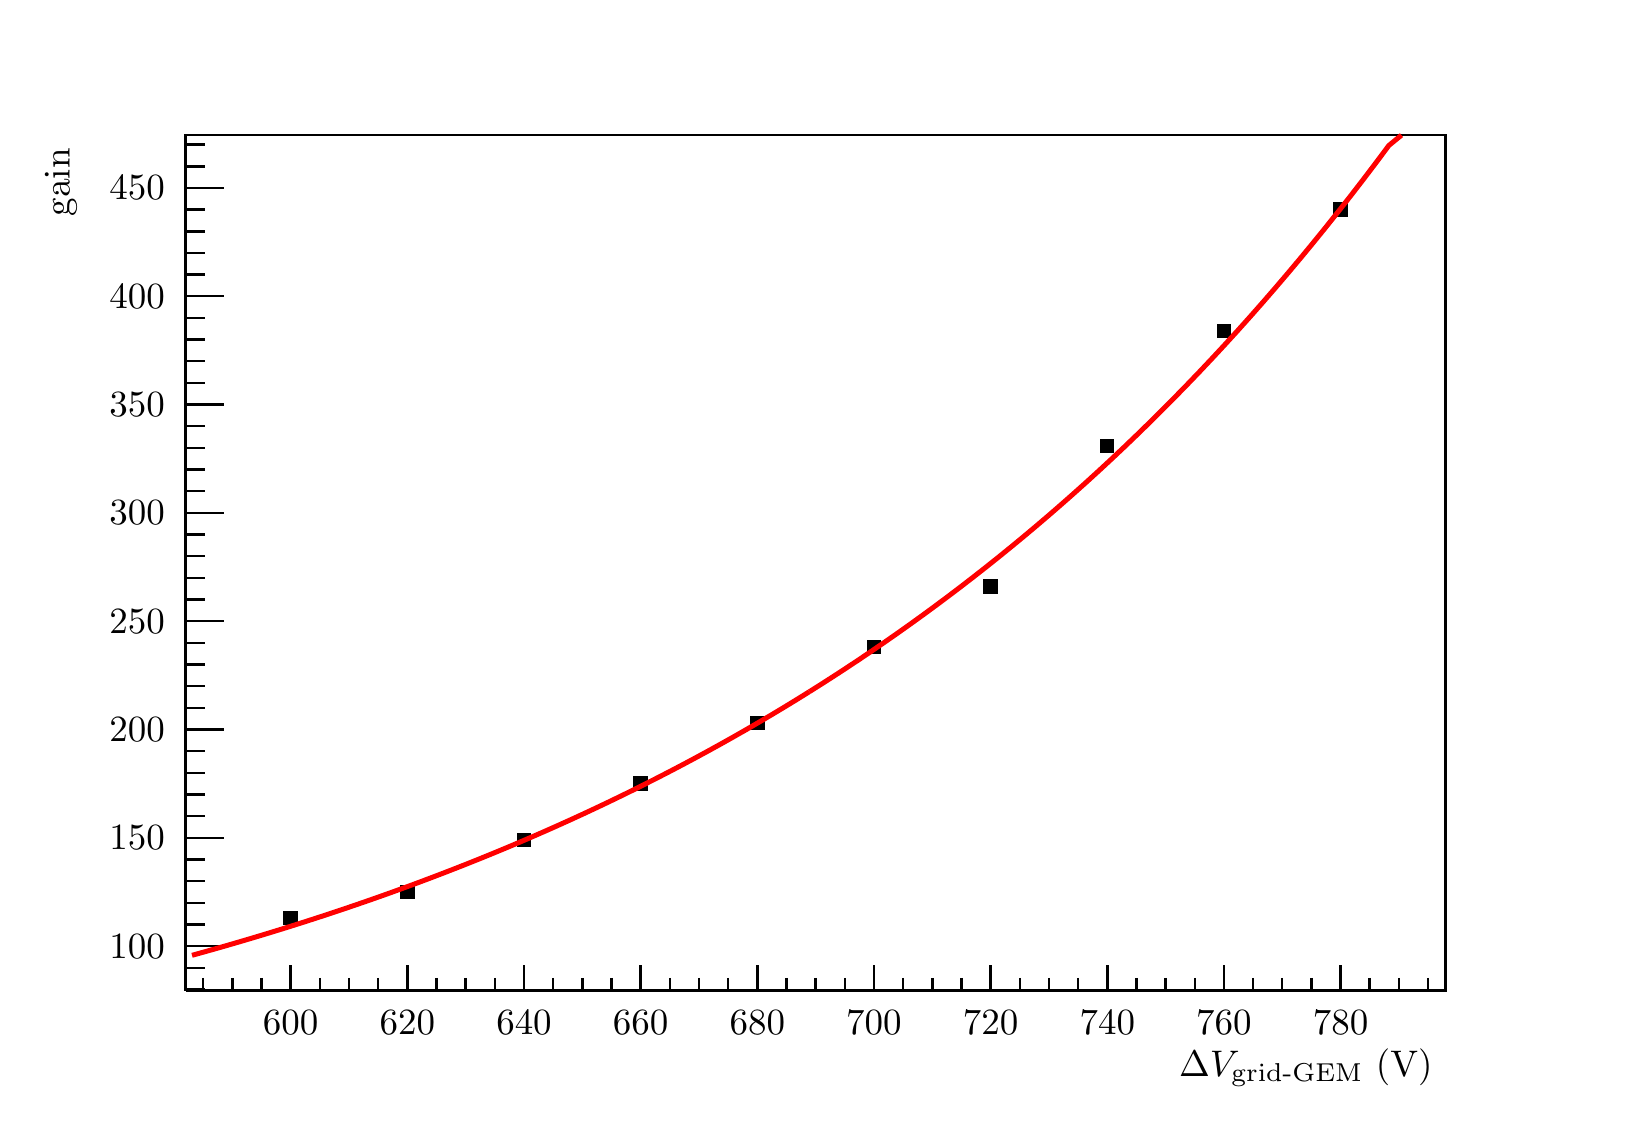
\begin{tikzpicture}
\pgfdeclareplotmark{cross} {
\pgfpathmoveto{\pgfpoint{-0.3\pgfplotmarksize}{\pgfplotmarksize}}
\pgfpathlineto{\pgfpoint{+0.3\pgfplotmarksize}{\pgfplotmarksize}}
\pgfpathlineto{\pgfpoint{+0.3\pgfplotmarksize}{0.3\pgfplotmarksize}}
\pgfpathlineto{\pgfpoint{+1\pgfplotmarksize}{0.3\pgfplotmarksize}}
\pgfpathlineto{\pgfpoint{+1\pgfplotmarksize}{-0.3\pgfplotmarksize}}
\pgfpathlineto{\pgfpoint{+0.3\pgfplotmarksize}{-0.3\pgfplotmarksize}}
\pgfpathlineto{\pgfpoint{+0.3\pgfplotmarksize}{-1.\pgfplotmarksize}}
\pgfpathlineto{\pgfpoint{-0.3\pgfplotmarksize}{-1.\pgfplotmarksize}}
\pgfpathlineto{\pgfpoint{-0.3\pgfplotmarksize}{-0.3\pgfplotmarksize}}
\pgfpathlineto{\pgfpoint{-1.\pgfplotmarksize}{-0.3\pgfplotmarksize}}
\pgfpathlineto{\pgfpoint{-1.\pgfplotmarksize}{0.3\pgfplotmarksize}}
\pgfpathlineto{\pgfpoint{-0.3\pgfplotmarksize}{0.3\pgfplotmarksize}}
\pgfpathclose
\pgfusepathqstroke
}
\pgfdeclareplotmark{cross*} {
\pgfpathmoveto{\pgfpoint{-0.3\pgfplotmarksize}{\pgfplotmarksize}}
\pgfpathlineto{\pgfpoint{+0.3\pgfplotmarksize}{\pgfplotmarksize}}
\pgfpathlineto{\pgfpoint{+0.3\pgfplotmarksize}{0.3\pgfplotmarksize}}
\pgfpathlineto{\pgfpoint{+1\pgfplotmarksize}{0.3\pgfplotmarksize}}
\pgfpathlineto{\pgfpoint{+1\pgfplotmarksize}{-0.3\pgfplotmarksize}}
\pgfpathlineto{\pgfpoint{+0.3\pgfplotmarksize}{-0.3\pgfplotmarksize}}
\pgfpathlineto{\pgfpoint{+0.3\pgfplotmarksize}{-1.\pgfplotmarksize}}
\pgfpathlineto{\pgfpoint{-0.3\pgfplotmarksize}{-1.\pgfplotmarksize}}
\pgfpathlineto{\pgfpoint{-0.3\pgfplotmarksize}{-0.3\pgfplotmarksize}}
\pgfpathlineto{\pgfpoint{-1.\pgfplotmarksize}{-0.3\pgfplotmarksize}}
\pgfpathlineto{\pgfpoint{-1.\pgfplotmarksize}{0.3\pgfplotmarksize}}
\pgfpathlineto{\pgfpoint{-0.3\pgfplotmarksize}{0.3\pgfplotmarksize}}
\pgfpathclose
\pgfusepathqfillstroke
}
\pgfdeclareplotmark{newstar} {
\pgfpathmoveto{\pgfqpoint{0pt}{\pgfplotmarksize}}
\pgfpathlineto{\pgfqpointpolar{44}{0.5\pgfplotmarksize}}
\pgfpathlineto{\pgfqpointpolar{18}{\pgfplotmarksize}}
\pgfpathlineto{\pgfqpointpolar{-20}{0.5\pgfplotmarksize}}
\pgfpathlineto{\pgfqpointpolar{-54}{\pgfplotmarksize}}
\pgfpathlineto{\pgfqpointpolar{-90}{0.5\pgfplotmarksize}}
\pgfpathlineto{\pgfqpointpolar{234}{\pgfplotmarksize}}
\pgfpathlineto{\pgfqpointpolar{198}{0.5\pgfplotmarksize}}
\pgfpathlineto{\pgfqpointpolar{162}{\pgfplotmarksize}}
\pgfpathlineto{\pgfqpointpolar{134}{0.5\pgfplotmarksize}}
\pgfpathclose
\pgfusepathqstroke
}
\pgfdeclareplotmark{newstar*} {
\pgfpathmoveto{\pgfqpoint{0pt}{\pgfplotmarksize}}
\pgfpathlineto{\pgfqpointpolar{44}{0.5\pgfplotmarksize}}
\pgfpathlineto{\pgfqpointpolar{18}{\pgfplotmarksize}}
\pgfpathlineto{\pgfqpointpolar{-20}{0.5\pgfplotmarksize}}
\pgfpathlineto{\pgfqpointpolar{-54}{\pgfplotmarksize}}
\pgfpathlineto{\pgfqpointpolar{-90}{0.5\pgfplotmarksize}}
\pgfpathlineto{\pgfqpointpolar{234}{\pgfplotmarksize}}
\pgfpathlineto{\pgfqpointpolar{198}{0.5\pgfplotmarksize}}
\pgfpathlineto{\pgfqpointpolar{162}{\pgfplotmarksize}}
\pgfpathlineto{\pgfqpointpolar{134}{0.5\pgfplotmarksize}}
\pgfpathclose
\pgfusepathqfillstroke
}
\definecolor{c}{rgb}{1,1,1};
\draw [color=c, fill=c] (0,0) rectangle (20,13.5817);
\draw [color=c, fill=c] (2,1.35817) rectangle (18,12.2235);
\definecolor{c}{rgb}{0,0,0};
\draw [c,line width=0.9] (2,1.35817) -- (2,12.2235) -- (18,12.2235) -- (18,1.35817) -- (2,1.35817);
\draw [c,line width=0.9] (2,1.35817) -- (18,1.35817);
\draw [c,line width=0.9] (3.33333,1.68413) -- (3.33333,1.35817);
\draw [c,line width=0.9] (3.7037,1.52115) -- (3.7037,1.35817);
\draw [c,line width=0.9] (4.07407,1.52115) -- (4.07407,1.35817);
\draw [c,line width=0.9] (4.44444,1.52115) -- (4.44444,1.35817);
\draw [c,line width=0.9] (4.81482,1.68413) -- (4.81482,1.35817);
\draw [c,line width=0.9] (5.18519,1.52115) -- (5.18519,1.35817);
\draw [c,line width=0.9] (5.55556,1.52115) -- (5.55556,1.35817);
\draw [c,line width=0.9] (5.92593,1.52115) -- (5.92593,1.35817);
\draw [c,line width=0.9] (6.2963,1.68413) -- (6.2963,1.35817);
\draw [c,line width=0.9] (6.66667,1.52115) -- (6.66667,1.35817);
\draw [c,line width=0.9] (7.03704,1.52115) -- (7.03704,1.35817);
\draw [c,line width=0.9] (7.40741,1.52115) -- (7.40741,1.35817);
\draw [c,line width=0.9] (7.77778,1.68413) -- (7.77778,1.35817);
\draw [c,line width=0.9] (8.14815,1.52115) -- (8.14815,1.35817);
\draw [c,line width=0.9] (8.51852,1.52115) -- (8.51852,1.35817);
\draw [c,line width=0.9] (8.88889,1.52115) -- (8.88889,1.35817);
\draw [c,line width=0.9] (9.25926,1.68413) -- (9.25926,1.35817);
\draw [c,line width=0.9] (9.62963,1.52115) -- (9.62963,1.35817);
\draw [c,line width=0.9] (10,1.52115) -- (10,1.35817);
\draw [c,line width=0.9] (10.3704,1.52115) -- (10.3704,1.35817);
\draw [c,line width=0.9] (10.7407,1.68413) -- (10.7407,1.35817);
\draw [c,line width=0.9] (11.1111,1.52115) -- (11.1111,1.35817);
\draw [c,line width=0.9] (11.4815,1.52115) -- (11.4815,1.35817);
\draw [c,line width=0.9] (11.8519,1.52115) -- (11.8519,1.35817);
\draw [c,line width=0.9] (12.2222,1.68413) -- (12.2222,1.35817);
\draw [c,line width=0.9] (12.5926,1.52115) -- (12.5926,1.35817);
\draw [c,line width=0.9] (12.963,1.52115) -- (12.963,1.35817);
\draw [c,line width=0.9] (13.3333,1.52115) -- (13.3333,1.35817);
\draw [c,line width=0.9] (13.7037,1.68413) -- (13.7037,1.35817);
\draw [c,line width=0.9] (14.0741,1.52115) -- (14.0741,1.35817);
\draw [c,line width=0.9] (14.4444,1.52115) -- (14.4444,1.35817);
\draw [c,line width=0.9] (14.8148,1.52115) -- (14.8148,1.35817);
\draw [c,line width=0.9] (15.1852,1.68413) -- (15.1852,1.35817);
\draw [c,line width=0.9] (15.5556,1.52115) -- (15.5556,1.35817);
\draw [c,line width=0.9] (15.9259,1.52115) -- (15.9259,1.35817);
\draw [c,line width=0.9] (16.2963,1.52115) -- (16.2963,1.35817);
\draw [c,line width=0.9] (16.6667,1.68413) -- (16.6667,1.35817);
\draw [c,line width=0.9] (3.33333,1.68413) -- (3.33333,1.35817);
\draw [c,line width=0.9] (2.96296,1.52115) -- (2.96296,1.35817);
\draw [c,line width=0.9] (2.59259,1.52115) -- (2.59259,1.35817);
\draw [c,line width=0.9] (2.22222,1.52115) -- (2.22222,1.35817);
\draw [c,line width=0.9] (16.6667,1.68413) -- (16.6667,1.35817);
\draw [c,line width=0.9] (17.037,1.52115) -- (17.037,1.35817);
\draw [c,line width=0.9] (17.4074,1.52115) -- (17.4074,1.35817);
\draw [c,line width=0.9] (17.7778,1.52115) -- (17.7778,1.35817);
\draw [anchor=base] (3.33333,0.801318) node[scale=1.3364, color=c, rotate=0]{600};
\draw [anchor=base] (4.81482,0.801318) node[scale=1.3364, color=c, rotate=0]{620};
\draw [anchor=base] (6.2963,0.801318) node[scale=1.3364, color=c, rotate=0]{640};
\draw [anchor=base] (7.77778,0.801318) node[scale=1.3364, color=c, rotate=0]{660};
\draw [anchor=base] (9.25926,0.801318) node[scale=1.3364, color=c, rotate=0]{680};
\draw [anchor=base] (10.7407,0.801318) node[scale=1.3364, color=c, rotate=0]{700};
\draw [anchor=base] (12.2222,0.801318) node[scale=1.3364, color=c, rotate=0]{720};
\draw [anchor=base] (13.7037,0.801318) node[scale=1.3364, color=c, rotate=0]{740};
\draw [anchor=base] (15.1852,0.801318) node[scale=1.3364, color=c, rotate=0]{760};
\draw [anchor=base] (16.6667,0.801318) node[scale=1.3364, color=c, rotate=0]{780};
\draw [anchor= east] (18,0.380287) node[scale=1.3364, color=c, rotate=0]{$\Delta V_{\text{grid-GEM}}\text{ (V)}$};
\draw [c,line width=0.9] (2,1.35817) -- (2,12.2235);
\draw [c,line width=0.9] (2.48,1.92486) -- (2,1.92486);
\draw [c,line width=0.9] (2.24,2.19995) -- (2,2.19995);
\draw [c,line width=0.9] (2.24,2.47505) -- (2,2.47505);
\draw [c,line width=0.9] (2.24,2.75015) -- (2,2.75015);
\draw [c,line width=0.9] (2.24,3.02524) -- (2,3.02524);
\draw [c,line width=0.9] (2.48,3.30034) -- (2,3.30034);
\draw [c,line width=0.9] (2.24,3.57544) -- (2,3.57544);
\draw [c,line width=0.9] (2.24,3.85054) -- (2,3.85054);
\draw [c,line width=0.9] (2.24,4.12563) -- (2,4.12563);
\draw [c,line width=0.9] (2.24,4.40073) -- (2,4.40073);
\draw [c,line width=0.9] (2.48,4.67583) -- (2,4.67583);
\draw [c,line width=0.9] (2.24,4.95093) -- (2,4.95093);
\draw [c,line width=0.9] (2.24,5.22602) -- (2,5.22602);
\draw [c,line width=0.9] (2.24,5.50112) -- (2,5.50112);
\draw [c,line width=0.9] (2.24,5.77622) -- (2,5.77622);
\draw [c,line width=0.9] (2.48,6.05131) -- (2,6.05131);
\draw [c,line width=0.9] (2.24,6.32641) -- (2,6.32641);
\draw [c,line width=0.9] (2.24,6.60151) -- (2,6.60151);
\draw [c,line width=0.9] (2.24,6.87661) -- (2,6.87661);
\draw [c,line width=0.9] (2.24,7.1517) -- (2,7.1517);
\draw [c,line width=0.9] (2.48,7.4268) -- (2,7.4268);
\draw [c,line width=0.9] (2.24,7.7019) -- (2,7.7019);
\draw [c,line width=0.9] (2.24,7.977) -- (2,7.977);
\draw [c,line width=0.9] (2.24,8.25209) -- (2,8.25209);
\draw [c,line width=0.9] (2.24,8.52719) -- (2,8.52719);
\draw [c,line width=0.9] (2.48,8.80229) -- (2,8.80229);
\draw [c,line width=0.9] (2.24,9.07738) -- (2,9.07738);
\draw [c,line width=0.9] (2.24,9.35248) -- (2,9.35248);
\draw [c,line width=0.9] (2.24,9.62758) -- (2,9.62758);
\draw [c,line width=0.9] (2.24,9.90268) -- (2,9.90268);
\draw [c,line width=0.9] (2.48,10.1778) -- (2,10.1778);
\draw [c,line width=0.9] (2.24,10.4529) -- (2,10.4529);
\draw [c,line width=0.9] (2.24,10.728) -- (2,10.728);
\draw [c,line width=0.9] (2.24,11.0031) -- (2,11.0031);
\draw [c,line width=0.9] (2.24,11.2782) -- (2,11.2782);
\draw [c,line width=0.9] (2.48,11.5533) -- (2,11.5533);
\draw [c,line width=0.9] (2.48,1.92486) -- (2,1.92486);
\draw [c,line width=0.9] (2.24,1.64976) -- (2,1.64976);
\draw [c,line width=0.9] (2.24,1.37466) -- (2,1.37466);
\draw [c,line width=0.9] (2.48,11.5533) -- (2,11.5533);
\draw [c,line width=0.9] (2.24,11.8284) -- (2,11.8284);
\draw [c,line width=0.9] (2.24,12.1035) -- (2,12.1035);
\draw [anchor= east] (1.9,1.92486) node[scale=1.3364, color=c, rotate=0]{100};
\draw [anchor= east] (1.9,3.30034) node[scale=1.3364, color=c, rotate=0]{150};
\draw [anchor= east] (1.9,4.67583) node[scale=1.3364, color=c, rotate=0]{200};
\draw [anchor= east] (1.9,6.05131) node[scale=1.3364, color=c, rotate=0]{250};
\draw [anchor= east] (1.9,7.4268) node[scale=1.3364, color=c, rotate=0]{300};
\draw [anchor= east] (1.9,8.80229) node[scale=1.3364, color=c, rotate=0]{350};
\draw [anchor= east] (1.9,10.1778) node[scale=1.3364, color=c, rotate=0]{400};
\draw [anchor= east] (1.9,11.5533) node[scale=1.3364, color=c, rotate=0]{450};
\draw [anchor= east] (0.416,12.2235) node[scale=1.3364, color=c, rotate=90]{gain};
\foreach \P in {(3.33333,2.28248), (4.81482,2.6126), (6.2963,3.27283), (7.77778,3.98809), (9.25926,4.75836), (10.7407,5.7212), (12.2222,6.49147), (13.7037,8.2796), (15.1852,9.73762), (16.6667,11.2782)}{\draw[mark options={color=c,fill=c},mark
 size=2.402402pt,mark=square*] plot coordinates {\P};}
\definecolor{c}{rgb}{1,0,0};
\draw [c,line width=1.8] (2.08,1.80756) -- (2.24,1.85202) -- (2.4,1.89723) -- (2.56,1.9432) -- (2.72,1.98995) -- (2.88,2.03749) -- (3.04,2.08583) -- (3.2,2.13499) -- (3.36,2.18497) -- (3.52,2.2358) -- (3.68,2.28749) -- (3.84,2.34005) -- (4,2.3935) --
 (4.16,2.44785) -- (4.32,2.50312) -- (4.48,2.55932) -- (4.64,2.61646) -- (4.8,2.67458) -- (4.96,2.73367) -- (5.12,2.79376) -- (5.28,2.85487) -- (5.44,2.91701) -- (5.6,2.9802) -- (5.76,3.04445) -- (5.92,3.10979) -- (6.08,3.17623) -- (6.24,3.24379) --
 (6.4,3.3125) -- (6.56,3.38236) -- (6.72,3.4534) -- (6.88,3.52564) -- (7.04,3.5991) -- (7.2,3.67381) -- (7.36,3.74977) -- (7.52,3.82701) -- (7.68,3.90556) -- (7.84,3.98544) -- (8,4.06666) -- (8.16,4.14925) -- (8.32,4.23324) -- (8.48,4.31865) --
 (8.64,4.4055) -- (8.8,4.49381) -- (8.96,4.58361) -- (9.12,4.67494) -- (9.28,4.7678) -- (9.44,4.86223) -- (9.6,4.95825) -- (9.76,5.0559) -- (9.92,5.15519);
\draw [c,line width=1.8] (9.92,5.15519) -- (10.08,5.25616) -- (10.24,5.35883) -- (10.4,5.46324) -- (10.56,5.56941) -- (10.72,5.67737) -- (10.88,5.78716) -- (11.04,5.89879) -- (11.2,6.01232) -- (11.36,6.12775) -- (11.52,6.24514) -- (11.68,6.36451) --
 (11.84,6.48589) -- (12,6.60933) -- (12.16,6.73484) -- (12.32,6.86248) -- (12.48,6.99227) -- (12.64,7.12425) -- (12.8,7.25846) -- (12.96,7.39493) -- (13.12,7.53371) -- (13.28,7.67483) -- (13.44,7.81833) -- (13.6,7.96426) -- (13.76,8.11265) --
 (13.92,8.26354) -- (14.08,8.41698) -- (14.24,8.57301) -- (14.4,8.73168) -- (14.56,8.89302) -- (14.72,9.05709) -- (14.88,9.22393) -- (15.04,9.39358) -- (15.2,9.5661) -- (15.36,9.74152) -- (15.52,9.91992) -- (15.68,10.1013) -- (15.84,10.2858) --
 (16,10.4734) -- (16.16,10.6641) -- (16.32,10.8581) -- (16.48,11.0553) -- (16.64,11.2559) -- (16.8,11.4598) -- (16.96,11.6672) -- (17.12,11.8781) -- (17.28,12.0926) -- (17.44,12.2235);
\end{tikzpicture}
}
  \caption{電子増幅率の$\Delta V_{\text{grid-GEM}}$依存性.}
  \label{fig::gain_grid_GEM_V_dep}
\end{figure}
%$\Delta V_{\text{grid-GEM}}$にたいして増幅率が単調に増加していることが分かる.
増幅率の変化は$0.00704\times{\Delta V_{\text{grid-GEM}}}^2-7.92\times{\Delta V_{\text{grid-GEM}}}+2330$とフィットできる.
%図\ref{fig::gain_GEM_V_dep}と同様に$\Delta V_{\rm grid-GEM} = $\SI{720}{\volt}で不連続性が見られる.
%これは,1時間ほどの時間のズレがあるためである.

\subsection{GEMによる電子増幅率}
GEM は絶縁体のフィルムの両面を銅で被覆し,微細な穴を開けたものである.
GEM の各面に電圧をかけることで高電場を形成し,電子のアバランシェ増幅を起こす.
$\Delta V_{\text{GEM}}$を変化させることで電子の増幅率が変化する.
最終的に得られる電子の増幅率の$\Delta V_{\text{GEM}}$依存性を図\ref{fig::gain_GEM_V_dep}に示す.
\begin{figure}
  \centering
% \includegraphics[clip, width=0.8\columnwidth]{gain_GEM_V_dep.eps}
  \scalebox{0.7}{\begin{tikzpicture}
\pgfdeclareplotmark{cross} {
\pgfpathmoveto{\pgfpoint{-0.3\pgfplotmarksize}{\pgfplotmarksize}}
\pgfpathlineto{\pgfpoint{+0.3\pgfplotmarksize}{\pgfplotmarksize}}
\pgfpathlineto{\pgfpoint{+0.3\pgfplotmarksize}{0.3\pgfplotmarksize}}
\pgfpathlineto{\pgfpoint{+1\pgfplotmarksize}{0.3\pgfplotmarksize}}
\pgfpathlineto{\pgfpoint{+1\pgfplotmarksize}{-0.3\pgfplotmarksize}}
\pgfpathlineto{\pgfpoint{+0.3\pgfplotmarksize}{-0.3\pgfplotmarksize}}
\pgfpathlineto{\pgfpoint{+0.3\pgfplotmarksize}{-1.\pgfplotmarksize}}
\pgfpathlineto{\pgfpoint{-0.3\pgfplotmarksize}{-1.\pgfplotmarksize}}
\pgfpathlineto{\pgfpoint{-0.3\pgfplotmarksize}{-0.3\pgfplotmarksize}}
\pgfpathlineto{\pgfpoint{-1.\pgfplotmarksize}{-0.3\pgfplotmarksize}}
\pgfpathlineto{\pgfpoint{-1.\pgfplotmarksize}{0.3\pgfplotmarksize}}
\pgfpathlineto{\pgfpoint{-0.3\pgfplotmarksize}{0.3\pgfplotmarksize}}
\pgfpathclose
\pgfusepathqstroke
}
\pgfdeclareplotmark{cross*} {
\pgfpathmoveto{\pgfpoint{-0.3\pgfplotmarksize}{\pgfplotmarksize}}
\pgfpathlineto{\pgfpoint{+0.3\pgfplotmarksize}{\pgfplotmarksize}}
\pgfpathlineto{\pgfpoint{+0.3\pgfplotmarksize}{0.3\pgfplotmarksize}}
\pgfpathlineto{\pgfpoint{+1\pgfplotmarksize}{0.3\pgfplotmarksize}}
\pgfpathlineto{\pgfpoint{+1\pgfplotmarksize}{-0.3\pgfplotmarksize}}
\pgfpathlineto{\pgfpoint{+0.3\pgfplotmarksize}{-0.3\pgfplotmarksize}}
\pgfpathlineto{\pgfpoint{+0.3\pgfplotmarksize}{-1.\pgfplotmarksize}}
\pgfpathlineto{\pgfpoint{-0.3\pgfplotmarksize}{-1.\pgfplotmarksize}}
\pgfpathlineto{\pgfpoint{-0.3\pgfplotmarksize}{-0.3\pgfplotmarksize}}
\pgfpathlineto{\pgfpoint{-1.\pgfplotmarksize}{-0.3\pgfplotmarksize}}
\pgfpathlineto{\pgfpoint{-1.\pgfplotmarksize}{0.3\pgfplotmarksize}}
\pgfpathlineto{\pgfpoint{-0.3\pgfplotmarksize}{0.3\pgfplotmarksize}}
\pgfpathclose
\pgfusepathqfillstroke
}
\pgfdeclareplotmark{newstar} {
\pgfpathmoveto{\pgfqpoint{0pt}{\pgfplotmarksize}}
\pgfpathlineto{\pgfqpointpolar{44}{0.5\pgfplotmarksize}}
\pgfpathlineto{\pgfqpointpolar{18}{\pgfplotmarksize}}
\pgfpathlineto{\pgfqpointpolar{-20}{0.5\pgfplotmarksize}}
\pgfpathlineto{\pgfqpointpolar{-54}{\pgfplotmarksize}}
\pgfpathlineto{\pgfqpointpolar{-90}{0.5\pgfplotmarksize}}
\pgfpathlineto{\pgfqpointpolar{234}{\pgfplotmarksize}}
\pgfpathlineto{\pgfqpointpolar{198}{0.5\pgfplotmarksize}}
\pgfpathlineto{\pgfqpointpolar{162}{\pgfplotmarksize}}
\pgfpathlineto{\pgfqpointpolar{134}{0.5\pgfplotmarksize}}
\pgfpathclose
\pgfusepathqstroke
}
\pgfdeclareplotmark{newstar*} {
\pgfpathmoveto{\pgfqpoint{0pt}{\pgfplotmarksize}}
\pgfpathlineto{\pgfqpointpolar{44}{0.5\pgfplotmarksize}}
\pgfpathlineto{\pgfqpointpolar{18}{\pgfplotmarksize}}
\pgfpathlineto{\pgfqpointpolar{-20}{0.5\pgfplotmarksize}}
\pgfpathlineto{\pgfqpointpolar{-54}{\pgfplotmarksize}}
\pgfpathlineto{\pgfqpointpolar{-90}{0.5\pgfplotmarksize}}
\pgfpathlineto{\pgfqpointpolar{234}{\pgfplotmarksize}}
\pgfpathlineto{\pgfqpointpolar{198}{0.5\pgfplotmarksize}}
\pgfpathlineto{\pgfqpointpolar{162}{\pgfplotmarksize}}
\pgfpathlineto{\pgfqpointpolar{134}{0.5\pgfplotmarksize}}
\pgfpathclose
\pgfusepathqfillstroke
}
\definecolor{c}{rgb}{1,1,1};
\draw [color=c, fill=c] (0,0) rectangle (20,13.5817);
\draw [color=c, fill=c] (2,1.35817) rectangle (18,12.2235);
\definecolor{c}{rgb}{0,0,0};
\draw [c,line width=0.9] (2,1.35817) -- (2,12.2235) -- (18,12.2235) -- (18,1.35817) -- (2,1.35817);
\draw [c,line width=0.9] (2,1.35817) -- (18,1.35817);
\draw [c,line width=0.9] (3.33333,1.68413) -- (3.33333,1.35817);
\draw [c,line width=0.9] (4.07407,1.52115) -- (4.07407,1.35817);
\draw [c,line width=0.9] (4.81482,1.52115) -- (4.81482,1.35817);
\draw [c,line width=0.9] (5.55556,1.52115) -- (5.55556,1.35817);
\draw [c,line width=0.9] (6.2963,1.68413) -- (6.2963,1.35817);
\draw [c,line width=0.9] (7.03704,1.52115) -- (7.03704,1.35817);
\draw [c,line width=0.9] (7.77778,1.52115) -- (7.77778,1.35817);
\draw [c,line width=0.9] (8.51852,1.52115) -- (8.51852,1.35817);
\draw [c,line width=0.9] (9.25926,1.68413) -- (9.25926,1.35817);
\draw [c,line width=0.9] (10,1.52115) -- (10,1.35817);
\draw [c,line width=0.9] (10.7407,1.52115) -- (10.7407,1.35817);
\draw [c,line width=0.9] (11.4815,1.52115) -- (11.4815,1.35817);
\draw [c,line width=0.9] (12.2222,1.68413) -- (12.2222,1.35817);
\draw [c,line width=0.9] (12.963,1.52115) -- (12.963,1.35817);
\draw [c,line width=0.9] (13.7037,1.52115) -- (13.7037,1.35817);
\draw [c,line width=0.9] (14.4444,1.52115) -- (14.4444,1.35817);
\draw [c,line width=0.9] (15.1852,1.68413) -- (15.1852,1.35817);
\draw [c,line width=0.9] (3.33333,1.68413) -- (3.33333,1.35817);
\draw [c,line width=0.9] (2.59259,1.52115) -- (2.59259,1.35817);
\draw [c,line width=0.9] (15.1852,1.68413) -- (15.1852,1.35817);
\draw [c,line width=0.9] (15.9259,1.52115) -- (15.9259,1.35817);
\draw [c,line width=0.9] (16.6667,1.52115) -- (16.6667,1.35817);
\draw [c,line width=0.9] (17.4074,1.52115) -- (17.4074,1.35817);
\draw [anchor=base] (3.33333,0.801318) node[scale=1.3364, color=c, rotate=0]{300};
\draw [anchor=base] (6.2963,0.801318) node[scale=1.3364, color=c, rotate=0]{320};
\draw [anchor=base] (9.25926,0.801318) node[scale=1.3364, color=c, rotate=0]{340};
\draw [anchor=base] (12.2222,0.801318) node[scale=1.3364, color=c, rotate=0]{360};
\draw [anchor=base] (15.1852,0.801318) node[scale=1.3364, color=c, rotate=0]{380};
\draw [anchor= east] (18,0.380287) node[scale=1.3364, color=c, rotate=0]{$\Delta V_{\text{GEM}}\text{ (V)}$};
\draw [c,line width=0.9] (2,1.35817) -- (2,12.2235);
\draw [c,line width=0.9] (2.48,1.77926) -- (2,1.77926);
\draw [c,line width=0.9] (2.24,2.06877) -- (2,2.06877);
\draw [c,line width=0.9] (2.24,2.35828) -- (2,2.35828);
\draw [c,line width=0.9] (2.24,2.64779) -- (2,2.64779);
\draw [c,line width=0.9] (2.24,2.9373) -- (2,2.9373);
\draw [c,line width=0.9] (2.48,3.22681) -- (2,3.22681);
\draw [c,line width=0.9] (2.24,3.51632) -- (2,3.51632);
\draw [c,line width=0.9] (2.24,3.80583) -- (2,3.80583);
\draw [c,line width=0.9] (2.24,4.09534) -- (2,4.09534);
\draw [c,line width=0.9] (2.24,4.38485) -- (2,4.38485);
\draw [c,line width=0.9] (2.48,4.67436) -- (2,4.67436);
\draw [c,line width=0.9] (2.24,4.96387) -- (2,4.96387);
\draw [c,line width=0.9] (2.24,5.25339) -- (2,5.25339);
\draw [c,line width=0.9] (2.24,5.5429) -- (2,5.5429);
\draw [c,line width=0.9] (2.24,5.83241) -- (2,5.83241);
\draw [c,line width=0.9] (2.48,6.12192) -- (2,6.12192);
\draw [c,line width=0.9] (2.24,6.41143) -- (2,6.41143);
\draw [c,line width=0.9] (2.24,6.70094) -- (2,6.70094);
\draw [c,line width=0.9] (2.24,6.99045) -- (2,6.99045);
\draw [c,line width=0.9] (2.24,7.27996) -- (2,7.27996);
\draw [c,line width=0.9] (2.48,7.56947) -- (2,7.56947);
\draw [c,line width=0.9] (2.24,7.85898) -- (2,7.85898);
\draw [c,line width=0.9] (2.24,8.14849) -- (2,8.14849);
\draw [c,line width=0.9] (2.24,8.438) -- (2,8.438);
\draw [c,line width=0.9] (2.24,8.72751) -- (2,8.72751);
\draw [c,line width=0.9] (2.48,9.01702) -- (2,9.01702);
\draw [c,line width=0.9] (2.24,9.30653) -- (2,9.30653);
\draw [c,line width=0.9] (2.24,9.59604) -- (2,9.59604);
\draw [c,line width=0.9] (2.24,9.88555) -- (2,9.88555);
\draw [c,line width=0.9] (2.24,10.1751) -- (2,10.1751);
\draw [c,line width=0.9] (2.48,10.4646) -- (2,10.4646);
\draw [c,line width=0.9] (2.24,10.7541) -- (2,10.7541);
\draw [c,line width=0.9] (2.24,11.0436) -- (2,11.0436);
\draw [c,line width=0.9] (2.24,11.3331) -- (2,11.3331);
\draw [c,line width=0.9] (2.24,11.6226) -- (2,11.6226);
\draw [c,line width=0.9] (2.48,11.9121) -- (2,11.9121);
\draw [c,line width=0.9] (2.48,1.77926) -- (2,1.77926);
\draw [c,line width=0.9] (2.24,1.48975) -- (2,1.48975);
\draw [c,line width=0.9] (2.48,11.9121) -- (2,11.9121);
\draw [c,line width=0.9] (2.24,12.2016) -- (2,12.2016);
\draw [anchor= east] (1.9,1.77926) node[scale=1.3364, color=c, rotate=0]{100};
\draw [anchor= east] (1.9,3.22681) node[scale=1.3364, color=c, rotate=0]{150};
\draw [anchor= east] (1.9,4.67436) node[scale=1.3364, color=c, rotate=0]{200};
\draw [anchor= east] (1.9,6.12192) node[scale=1.3364, color=c, rotate=0]{250};
\draw [anchor= east] (1.9,7.56947) node[scale=1.3364, color=c, rotate=0]{300};
\draw [anchor= east] (1.9,9.01702) node[scale=1.3364, color=c, rotate=0]{350};
\draw [anchor= east] (1.9,10.4646) node[scale=1.3364, color=c, rotate=0]{400};
\draw [anchor= east] (1.9,11.9121) node[scale=1.3364, color=c, rotate=0]{450};
\draw [anchor= east] (0.416,12.2235) node[scale=1.3364, color=c, rotate=90]{gain};
\foreach \P in {(3.33333,2.30038), (4.81482,3.13996), (6.2963,3.86373), (7.77778,4.58751), (9.25926,5.48499), (10.7407,5.7745), (12.2222,7.45367), (13.7037,8.40905), (15.1852,9.62499), (16.6667,11.2752)}{\draw[mark options={color=c,fill=c},mark
 size=2.402402pt,mark=square*] plot coordinates {\P};}
\definecolor{c}{rgb}{1,0,0};
\draw [c,line width=1.8] (2.08,2.18828) -- (2.24,2.22879) -- (2.4,2.27057) -- (2.56,2.31361) -- (2.72,2.35792) -- (2.88,2.4035) -- (3.04,2.45035) -- (3.2,2.49846) -- (3.36,2.54784) -- (3.52,2.59849) -- (3.68,2.65041) -- (3.84,2.70359) -- (4,2.75804)
 -- (4.16,2.81376) -- (4.32,2.87074) -- (4.48,2.929) -- (4.64,2.98852) -- (4.8,3.0493) -- (4.96,3.11136) -- (5.12,3.17468) -- (5.28,3.23927) -- (5.44,3.30513) -- (5.6,3.37225) -- (5.76,3.44065) -- (5.92,3.51031) -- (6.08,3.58123) -- (6.24,3.65343) --
 (6.4,3.72689) -- (6.56,3.80162) -- (6.72,3.87761) -- (6.88,3.95488) -- (7.04,4.03341) -- (7.2,4.11321) -- (7.36,4.19427) -- (7.52,4.27661) -- (7.68,4.36021) -- (7.84,4.44508) -- (8,4.53121) -- (8.16,4.61861) -- (8.32,4.70728) -- (8.48,4.79722) --
 (8.64,4.88843) -- (8.8,4.9809) -- (8.96,5.07464) -- (9.12,5.16965) -- (9.28,5.26592) -- (9.44,5.36346) -- (9.6,5.46227) -- (9.76,5.56235) -- (9.92,5.6637);
\draw [c,line width=1.8] (9.92,5.6637) -- (10.08,5.76631) -- (10.24,5.87019) -- (10.4,5.97533) -- (10.56,6.08175) -- (10.72,6.18943) -- (10.88,6.29838) -- (11.04,6.4086) -- (11.2,6.52008) -- (11.36,6.63283) -- (11.52,6.74685) -- (11.68,6.86213) --
 (11.84,6.97869) -- (12,7.09651) -- (12.16,7.2156) -- (12.32,7.33595) -- (12.48,7.45758) -- (12.64,7.58047) -- (12.8,7.70462) -- (12.96,7.83005) -- (13.12,7.95674) -- (13.28,8.0847) -- (13.44,8.21393) -- (13.6,8.34442) -- (13.76,8.47619) --
 (13.92,8.60921) -- (14.08,8.74351) -- (14.24,8.87908) -- (14.4,9.01591) -- (14.56,9.15401) -- (14.72,9.29337) -- (14.88,9.43401) -- (15.04,9.57591) -- (15.2,9.71908) -- (15.36,9.86351) -- (15.52,10.0092) -- (15.68,10.1562) -- (15.84,10.3044) --
 (16,10.4539) -- (16.16,10.6047) -- (16.32,10.7567) -- (16.48,10.9101) -- (16.64,11.0646) -- (16.8,11.2205) -- (16.96,11.3776) -- (17.12,11.536) -- (17.28,11.6956) -- (17.44,11.8565) -- (17.6,12.0187) -- (17.76,12.1821);
\definecolor{c}{rgb}{0,0,0};
\foreach \P in {(3.33333,2.30038), (4.81482,3.13996), (6.2963,3.86373), (7.77778,4.58751), (9.25926,5.48499), (10.7407,5.7745), (12.2222,7.45367), (13.7037,8.40905), (15.1852,9.62499), (16.6667,11.2752)}{\draw[mark options={color=c,fill=c},mark
 size=2.402402pt,mark=square*] plot coordinates {\P};}
\end{tikzpicture}
}
  \caption{電子増幅率の$\Delta V_{\text{GEM}}$依存性.}
  \label{fig::gain_GEM_V_dep}
\end{figure}
%$\Delta V_{\rm GEM}$に対して増幅率が単調に増加していることが分かる.
増幅率の変化は$0.0188\times{\Delta V_{\text{GEM}}}^2-0.67\times{\Delta V_{\text{GEM}}}+1340$とフィットできる.
$\Delta V_{\rm GEM} = 350 {\rm V}$とそれ以外では測定するタイミングが2時間ほどずれている.
そのため,図\ref{fig::gain_GEM_V_dep}で$V_{\text{GEM}} = 350 {\text{V}}$のみ不連続に変化している.

\subsection{GEMと$\mu$-PICとの電位差による電子の増幅率}
$\Delta V_{\text{GEM-}\mu\text{-PIC}}$によってGEM で増幅された電子の$\mu$-PICによる収集率が変化する.
最終的に得られる電子の増幅率の$\Delta V_{\text{GEM-}\mu\text{-PIC}}$依存性を図\ref{fig::gain_GEM_uPIC_V_dep}に示す.
\begin{figure}
  \centering
  \scalebox{0.7}{\begin{tikzpicture}
\pgfdeclareplotmark{cross} {
\pgfpathmoveto{\pgfpoint{-0.3\pgfplotmarksize}{\pgfplotmarksize}}
\pgfpathlineto{\pgfpoint{+0.3\pgfplotmarksize}{\pgfplotmarksize}}
\pgfpathlineto{\pgfpoint{+0.3\pgfplotmarksize}{0.3\pgfplotmarksize}}
\pgfpathlineto{\pgfpoint{+1\pgfplotmarksize}{0.3\pgfplotmarksize}}
\pgfpathlineto{\pgfpoint{+1\pgfplotmarksize}{-0.3\pgfplotmarksize}}
\pgfpathlineto{\pgfpoint{+0.3\pgfplotmarksize}{-0.3\pgfplotmarksize}}
\pgfpathlineto{\pgfpoint{+0.3\pgfplotmarksize}{-1.\pgfplotmarksize}}
\pgfpathlineto{\pgfpoint{-0.3\pgfplotmarksize}{-1.\pgfplotmarksize}}
\pgfpathlineto{\pgfpoint{-0.3\pgfplotmarksize}{-0.3\pgfplotmarksize}}
\pgfpathlineto{\pgfpoint{-1.\pgfplotmarksize}{-0.3\pgfplotmarksize}}
\pgfpathlineto{\pgfpoint{-1.\pgfplotmarksize}{0.3\pgfplotmarksize}}
\pgfpathlineto{\pgfpoint{-0.3\pgfplotmarksize}{0.3\pgfplotmarksize}}
\pgfpathclose
\pgfusepathqstroke
}
\pgfdeclareplotmark{cross*} {
\pgfpathmoveto{\pgfpoint{-0.3\pgfplotmarksize}{\pgfplotmarksize}}
\pgfpathlineto{\pgfpoint{+0.3\pgfplotmarksize}{\pgfplotmarksize}}
\pgfpathlineto{\pgfpoint{+0.3\pgfplotmarksize}{0.3\pgfplotmarksize}}
\pgfpathlineto{\pgfpoint{+1\pgfplotmarksize}{0.3\pgfplotmarksize}}
\pgfpathlineto{\pgfpoint{+1\pgfplotmarksize}{-0.3\pgfplotmarksize}}
\pgfpathlineto{\pgfpoint{+0.3\pgfplotmarksize}{-0.3\pgfplotmarksize}}
\pgfpathlineto{\pgfpoint{+0.3\pgfplotmarksize}{-1.\pgfplotmarksize}}
\pgfpathlineto{\pgfpoint{-0.3\pgfplotmarksize}{-1.\pgfplotmarksize}}
\pgfpathlineto{\pgfpoint{-0.3\pgfplotmarksize}{-0.3\pgfplotmarksize}}
\pgfpathlineto{\pgfpoint{-1.\pgfplotmarksize}{-0.3\pgfplotmarksize}}
\pgfpathlineto{\pgfpoint{-1.\pgfplotmarksize}{0.3\pgfplotmarksize}}
\pgfpathlineto{\pgfpoint{-0.3\pgfplotmarksize}{0.3\pgfplotmarksize}}
\pgfpathclose
\pgfusepathqfillstroke
}
\pgfdeclareplotmark{newstar} {
\pgfpathmoveto{\pgfqpoint{0pt}{\pgfplotmarksize}}
\pgfpathlineto{\pgfqpointpolar{44}{0.5\pgfplotmarksize}}
\pgfpathlineto{\pgfqpointpolar{18}{\pgfplotmarksize}}
\pgfpathlineto{\pgfqpointpolar{-20}{0.5\pgfplotmarksize}}
\pgfpathlineto{\pgfqpointpolar{-54}{\pgfplotmarksize}}
\pgfpathlineto{\pgfqpointpolar{-90}{0.5\pgfplotmarksize}}
\pgfpathlineto{\pgfqpointpolar{234}{\pgfplotmarksize}}
\pgfpathlineto{\pgfqpointpolar{198}{0.5\pgfplotmarksize}}
\pgfpathlineto{\pgfqpointpolar{162}{\pgfplotmarksize}}
\pgfpathlineto{\pgfqpointpolar{134}{0.5\pgfplotmarksize}}
\pgfpathclose
\pgfusepathqstroke
}
\pgfdeclareplotmark{newstar*} {
\pgfpathmoveto{\pgfqpoint{0pt}{\pgfplotmarksize}}
\pgfpathlineto{\pgfqpointpolar{44}{0.5\pgfplotmarksize}}
\pgfpathlineto{\pgfqpointpolar{18}{\pgfplotmarksize}}
\pgfpathlineto{\pgfqpointpolar{-20}{0.5\pgfplotmarksize}}
\pgfpathlineto{\pgfqpointpolar{-54}{\pgfplotmarksize}}
\pgfpathlineto{\pgfqpointpolar{-90}{0.5\pgfplotmarksize}}
\pgfpathlineto{\pgfqpointpolar{234}{\pgfplotmarksize}}
\pgfpathlineto{\pgfqpointpolar{198}{0.5\pgfplotmarksize}}
\pgfpathlineto{\pgfqpointpolar{162}{\pgfplotmarksize}}
\pgfpathlineto{\pgfqpointpolar{134}{0.5\pgfplotmarksize}}
\pgfpathclose
\pgfusepathqfillstroke
}
\definecolor{c}{rgb}{1,1,1};
\draw [color=c, fill=c] (0,0) rectangle (20,13.5817);
\draw [color=c, fill=c] (2,1.35817) rectangle (18,12.2235);
\definecolor{c}{rgb}{0,0,0};
\draw [c,line width=0.9] (2,1.35817) -- (2,12.2235) -- (18,12.2235) -- (18,1.35817) -- (2,1.35817);
\draw [c,line width=0.9] (2,1.35817) -- (18,1.35817);
\draw [c,line width=0.9] (3.33333,1.68413) -- (3.33333,1.35817);
\draw [c,line width=0.9] (4,1.52115) -- (4,1.35817);
\draw [c,line width=0.9] (4.66667,1.52115) -- (4.66667,1.35817);
\draw [c,line width=0.9] (5.33333,1.52115) -- (5.33333,1.35817);
\draw [c,line width=0.9] (6,1.52115) -- (6,1.35817);
\draw [c,line width=0.9] (6.66667,1.68413) -- (6.66667,1.35817);
\draw [c,line width=0.9] (7.33333,1.52115) -- (7.33333,1.35817);
\draw [c,line width=0.9] (8,1.52115) -- (8,1.35817);
\draw [c,line width=0.9] (8.66667,1.52115) -- (8.66667,1.35817);
\draw [c,line width=0.9] (9.33333,1.52115) -- (9.33333,1.35817);
\draw [c,line width=0.9] (10,1.68413) -- (10,1.35817);
\draw [c,line width=0.9] (10.6667,1.52115) -- (10.6667,1.35817);
\draw [c,line width=0.9] (11.3333,1.52115) -- (11.3333,1.35817);
\draw [c,line width=0.9] (12,1.52115) -- (12,1.35817);
\draw [c,line width=0.9] (12.6667,1.52115) -- (12.6667,1.35817);
\draw [c,line width=0.9] (13.3333,1.68413) -- (13.3333,1.35817);
\draw [c,line width=0.9] (14,1.52115) -- (14,1.35817);
\draw [c,line width=0.9] (14.6667,1.52115) -- (14.6667,1.35817);
\draw [c,line width=0.9] (15.3333,1.52115) -- (15.3333,1.35817);
\draw [c,line width=0.9] (16,1.52115) -- (16,1.35817);
\draw [c,line width=0.9] (16.6667,1.68413) -- (16.6667,1.35817);
\draw [c,line width=0.9] (3.33333,1.68413) -- (3.33333,1.35817);
\draw [c,line width=0.9] (2.66667,1.52115) -- (2.66667,1.35817);
\draw [c,line width=0.9] (2,1.52115) -- (2,1.35817);
\draw [c,line width=0.9] (16.6667,1.68413) -- (16.6667,1.35817);
\draw [c,line width=0.9] (17.3333,1.52115) -- (17.3333,1.35817);
\draw [anchor=base] (3.33333,0.801318) node[scale=1.3364, color=c, rotate=0]{550};
\draw [anchor=base] (6.66667,0.801318) node[scale=1.3364, color=c, rotate=0]{600};
\draw [anchor=base] (10,0.801318) node[scale=1.3364, color=c, rotate=0]{650};
\draw [anchor=base] (13.3333,0.801318) node[scale=1.3364, color=c, rotate=0]{700};
\draw [anchor=base] (16.6667,0.801318) node[scale=1.3364, color=c, rotate=0]{750};
\draw [anchor= east] (18,0.380287) node[scale=1.3364, color=c, rotate=0]{$\Delta V_{\text{GEM}-\mu\text{-PIC}}\text{ (V)}$};
\draw [c,line width=0.9] (2,1.35817) -- (2,12.2235);
\draw [c,line width=0.9] (2.48,1.73975) -- (2,1.73975);
\draw [c,line width=0.9] (2.24,2.02784) -- (2,2.02784);
\draw [c,line width=0.9] (2.24,2.31593) -- (2,2.31593);
\draw [c,line width=0.9] (2.24,2.60401) -- (2,2.60401);
\draw [c,line width=0.9] (2.48,2.8921) -- (2,2.8921);
\draw [c,line width=0.9] (2.24,3.18019) -- (2,3.18019);
\draw [c,line width=0.9] (2.24,3.46827) -- (2,3.46827);
\draw [c,line width=0.9] (2.24,3.75636) -- (2,3.75636);
\draw [c,line width=0.9] (2.48,4.04445) -- (2,4.04445);
\draw [c,line width=0.9] (2.24,4.33253) -- (2,4.33253);
\draw [c,line width=0.9] (2.24,4.62062) -- (2,4.62062);
\draw [c,line width=0.9] (2.24,4.9087) -- (2,4.9087);
\draw [c,line width=0.9] (2.48,5.19679) -- (2,5.19679);
\draw [c,line width=0.9] (2.24,5.48488) -- (2,5.48488);
\draw [c,line width=0.9] (2.24,5.77296) -- (2,5.77296);
\draw [c,line width=0.9] (2.24,6.06105) -- (2,6.06105);
\draw [c,line width=0.9] (2.48,6.34914) -- (2,6.34914);
\draw [c,line width=0.9] (2.24,6.63722) -- (2,6.63722);
\draw [c,line width=0.9] (2.24,6.92531) -- (2,6.92531);
\draw [c,line width=0.9] (2.24,7.2134) -- (2,7.2134);
\draw [c,line width=0.9] (2.48,7.50148) -- (2,7.50148);
\draw [c,line width=0.9] (2.24,7.78957) -- (2,7.78957);
\draw [c,line width=0.9] (2.24,8.07766) -- (2,8.07766);
\draw [c,line width=0.9] (2.24,8.36574) -- (2,8.36574);
\draw [c,line width=0.9] (2.48,8.65383) -- (2,8.65383);
\draw [c,line width=0.9] (2.24,8.94191) -- (2,8.94191);
\draw [c,line width=0.9] (2.24,9.23) -- (2,9.23);
\draw [c,line width=0.9] (2.24,9.51809) -- (2,9.51809);
\draw [c,line width=0.9] (2.48,9.80617) -- (2,9.80617);
\draw [c,line width=0.9] (2.24,10.0943) -- (2,10.0943);
\draw [c,line width=0.9] (2.24,10.3823) -- (2,10.3823);
\draw [c,line width=0.9] (2.24,10.6704) -- (2,10.6704);
\draw [c,line width=0.9] (2.48,10.9585) -- (2,10.9585);
\draw [c,line width=0.9] (2.24,11.2466) -- (2,11.2466);
\draw [c,line width=0.9] (2.24,11.5347) -- (2,11.5347);
\draw [c,line width=0.9] (2.24,11.8228) -- (2,11.8228);
\draw [c,line width=0.9] (2.48,12.1109) -- (2,12.1109);
\draw [c,line width=0.9] (2.48,1.73975) -- (2,1.73975);
\draw [c,line width=0.9] (2.24,1.45167) -- (2,1.45167);
\draw [c,line width=0.9] (2.48,12.1109) -- (2,12.1109);
\draw [anchor= east] (1.9,1.73975) node[scale=1.3364, color=c, rotate=0]{160};
\draw [anchor= east] (1.9,2.8921) node[scale=1.3364, color=c, rotate=0]{180};
\draw [anchor= east] (1.9,4.04445) node[scale=1.3364, color=c, rotate=0]{200};
\draw [anchor= east] (1.9,5.19679) node[scale=1.3364, color=c, rotate=0]{220};
\draw [anchor= east] (1.9,6.34914) node[scale=1.3364, color=c, rotate=0]{240};
\draw [anchor= east] (1.9,7.50148) node[scale=1.3364, color=c, rotate=0]{260};
\draw [anchor= east] (1.9,8.65383) node[scale=1.3364, color=c, rotate=0]{280};
\draw [anchor= east] (1.9,9.80617) node[scale=1.3364, color=c, rotate=0]{300};
\draw [anchor= east] (1.9,10.9585) node[scale=1.3364, color=c, rotate=0]{320};
\draw [anchor= east] (1.9,12.1109) node[scale=1.3364, color=c, rotate=0]{340};
\draw [anchor= east] (0.416,12.2235) node[scale=1.3364, color=c, rotate=90]{gain};
\foreach \P in {(3.33333,2.31593), (6.66667,4.67824), (10,6.2339), (13.3333,9.11477), (16.6667,11.2466)}{\draw[mark options={color=c,fill=c},mark size=2.402402pt,mark=square*] plot coordinates {\P};}
\end{tikzpicture}
}
  \caption{電子増幅率の$\Delta V_{\text{GEM-}\mu\text{-PIC}}$依存性.}
  \label{fig::gain_GEM_uPIC_V_dep}
\end{figure}
増幅率の変化は$0.767\times{\Delta V_{\text{GEM-}\mu\text{-PIC}}}$とフィットできる.

\subsection{$\mu$-PICによる電子増幅率}
電子は$\mu$-PICで読み出される直前に,$\mu$-PICによって作られた高電場によって増幅される.
最終的に得られる電子の増幅率の$\mu$-PICのanode電極にかける電圧 ($V_{\mu\text{-PIC}}$) に対する依存性を
図\ref{fig::gain_uPIC_V_dep}に示す.
\begin{figure}
  \centering
%  \includegraphics[clip, width=0.8\columnwidth]{gain_uPIC_V_dep.eps}
  \scalebox{0.7}{\begin{tikzpicture}
\pgfdeclareplotmark{cross} {
\pgfpathmoveto{\pgfpoint{-0.3\pgfplotmarksize}{\pgfplotmarksize}}
\pgfpathlineto{\pgfpoint{+0.3\pgfplotmarksize}{\pgfplotmarksize}}
\pgfpathlineto{\pgfpoint{+0.3\pgfplotmarksize}{0.3\pgfplotmarksize}}
\pgfpathlineto{\pgfpoint{+1\pgfplotmarksize}{0.3\pgfplotmarksize}}
\pgfpathlineto{\pgfpoint{+1\pgfplotmarksize}{-0.3\pgfplotmarksize}}
\pgfpathlineto{\pgfpoint{+0.3\pgfplotmarksize}{-0.3\pgfplotmarksize}}
\pgfpathlineto{\pgfpoint{+0.3\pgfplotmarksize}{-1.\pgfplotmarksize}}
\pgfpathlineto{\pgfpoint{-0.3\pgfplotmarksize}{-1.\pgfplotmarksize}}
\pgfpathlineto{\pgfpoint{-0.3\pgfplotmarksize}{-0.3\pgfplotmarksize}}
\pgfpathlineto{\pgfpoint{-1.\pgfplotmarksize}{-0.3\pgfplotmarksize}}
\pgfpathlineto{\pgfpoint{-1.\pgfplotmarksize}{0.3\pgfplotmarksize}}
\pgfpathlineto{\pgfpoint{-0.3\pgfplotmarksize}{0.3\pgfplotmarksize}}
\pgfpathclose
\pgfusepathqstroke
}
\pgfdeclareplotmark{cross*} {
\pgfpathmoveto{\pgfpoint{-0.3\pgfplotmarksize}{\pgfplotmarksize}}
\pgfpathlineto{\pgfpoint{+0.3\pgfplotmarksize}{\pgfplotmarksize}}
\pgfpathlineto{\pgfpoint{+0.3\pgfplotmarksize}{0.3\pgfplotmarksize}}
\pgfpathlineto{\pgfpoint{+1\pgfplotmarksize}{0.3\pgfplotmarksize}}
\pgfpathlineto{\pgfpoint{+1\pgfplotmarksize}{-0.3\pgfplotmarksize}}
\pgfpathlineto{\pgfpoint{+0.3\pgfplotmarksize}{-0.3\pgfplotmarksize}}
\pgfpathlineto{\pgfpoint{+0.3\pgfplotmarksize}{-1.\pgfplotmarksize}}
\pgfpathlineto{\pgfpoint{-0.3\pgfplotmarksize}{-1.\pgfplotmarksize}}
\pgfpathlineto{\pgfpoint{-0.3\pgfplotmarksize}{-0.3\pgfplotmarksize}}
\pgfpathlineto{\pgfpoint{-1.\pgfplotmarksize}{-0.3\pgfplotmarksize}}
\pgfpathlineto{\pgfpoint{-1.\pgfplotmarksize}{0.3\pgfplotmarksize}}
\pgfpathlineto{\pgfpoint{-0.3\pgfplotmarksize}{0.3\pgfplotmarksize}}
\pgfpathclose
\pgfusepathqfillstroke
}
\pgfdeclareplotmark{newstar} {
\pgfpathmoveto{\pgfqpoint{0pt}{\pgfplotmarksize}}
\pgfpathlineto{\pgfqpointpolar{44}{0.5\pgfplotmarksize}}
\pgfpathlineto{\pgfqpointpolar{18}{\pgfplotmarksize}}
\pgfpathlineto{\pgfqpointpolar{-20}{0.5\pgfplotmarksize}}
\pgfpathlineto{\pgfqpointpolar{-54}{\pgfplotmarksize}}
\pgfpathlineto{\pgfqpointpolar{-90}{0.5\pgfplotmarksize}}
\pgfpathlineto{\pgfqpointpolar{234}{\pgfplotmarksize}}
\pgfpathlineto{\pgfqpointpolar{198}{0.5\pgfplotmarksize}}
\pgfpathlineto{\pgfqpointpolar{162}{\pgfplotmarksize}}
\pgfpathlineto{\pgfqpointpolar{134}{0.5\pgfplotmarksize}}
\pgfpathclose
\pgfusepathqstroke
}
\pgfdeclareplotmark{newstar*} {
\pgfpathmoveto{\pgfqpoint{0pt}{\pgfplotmarksize}}
\pgfpathlineto{\pgfqpointpolar{44}{0.5\pgfplotmarksize}}
\pgfpathlineto{\pgfqpointpolar{18}{\pgfplotmarksize}}
\pgfpathlineto{\pgfqpointpolar{-20}{0.5\pgfplotmarksize}}
\pgfpathlineto{\pgfqpointpolar{-54}{\pgfplotmarksize}}
\pgfpathlineto{\pgfqpointpolar{-90}{0.5\pgfplotmarksize}}
\pgfpathlineto{\pgfqpointpolar{234}{\pgfplotmarksize}}
\pgfpathlineto{\pgfqpointpolar{198}{0.5\pgfplotmarksize}}
\pgfpathlineto{\pgfqpointpolar{162}{\pgfplotmarksize}}
\pgfpathlineto{\pgfqpointpolar{134}{0.5\pgfplotmarksize}}
\pgfpathclose
\pgfusepathqfillstroke
}
\definecolor{c}{rgb}{1,1,1};
\draw [color=c, fill=c] (0,0) rectangle (20,13.5817);
\draw [color=c, fill=c] (2,1.35817) rectangle (18,12.2235);
\definecolor{c}{rgb}{0,0,0};
\draw [c,line width=0.9] (2,1.35817) -- (2,12.2235) -- (18,12.2235) -- (18,1.35817) -- (2,1.35817);
\draw [c,line width=0.9] (2,1.35817) -- (18,1.35817);
\draw [c,line width=0.9] (4.81482,1.68413) -- (4.81482,1.35817);
\draw [c,line width=0.9] (5.55556,1.52115) -- (5.55556,1.35817);
\draw [c,line width=0.9] (6.2963,1.52115) -- (6.2963,1.35817);
\draw [c,line width=0.9] (7.03704,1.52115) -- (7.03704,1.35817);
\draw [c,line width=0.9] (7.77778,1.68413) -- (7.77778,1.35817);
\draw [c,line width=0.9] (8.51852,1.52115) -- (8.51852,1.35817);
\draw [c,line width=0.9] (9.25926,1.52115) -- (9.25926,1.35817);
\draw [c,line width=0.9] (10,1.52115) -- (10,1.35817);
\draw [c,line width=0.9] (10.7407,1.68413) -- (10.7407,1.35817);
\draw [c,line width=0.9] (11.4815,1.52115) -- (11.4815,1.35817);
\draw [c,line width=0.9] (12.2222,1.52115) -- (12.2222,1.35817);
\draw [c,line width=0.9] (12.963,1.52115) -- (12.963,1.35817);
\draw [c,line width=0.9] (13.7037,1.68413) -- (13.7037,1.35817);
\draw [c,line width=0.9] (14.4444,1.52115) -- (14.4444,1.35817);
\draw [c,line width=0.9] (15.1852,1.52115) -- (15.1852,1.35817);
\draw [c,line width=0.9] (15.9259,1.52115) -- (15.9259,1.35817);
\draw [c,line width=0.9] (16.6667,1.68413) -- (16.6667,1.35817);
\draw [c,line width=0.9] (4.81482,1.68413) -- (4.81482,1.35817);
\draw [c,line width=0.9] (4.07407,1.52115) -- (4.07407,1.35817);
\draw [c,line width=0.9] (3.33333,1.52115) -- (3.33333,1.35817);
\draw [c,line width=0.9] (2.59259,1.52115) -- (2.59259,1.35817);
\draw [c,line width=0.9] (16.6667,1.68413) -- (16.6667,1.35817);
\draw [c,line width=0.9] (17.4074,1.52115) -- (17.4074,1.35817);
\draw [anchor=base] (4.81482,0.801318) node[scale=1.3364, color=c, rotate=0]{360};
\draw [anchor=base] (7.77778,0.801318) node[scale=1.3364, color=c, rotate=0]{380};
\draw [anchor=base] (10.7407,0.801318) node[scale=1.3364, color=c, rotate=0]{400};
\draw [anchor=base] (13.7037,0.801318) node[scale=1.3364, color=c, rotate=0]{420};
\draw [anchor=base] (16.6667,0.801318) node[scale=1.3364, color=c, rotate=0]{440};
\draw [anchor= east] (18,0.380287) node[scale=1.3364, color=c, rotate=0]{$V_{\mu\text{-PIC}}\text{ (V)}$};
\draw [c,line width=0.9] (2,1.35817) -- (2,12.2235);
\draw [c,line width=0.9] (2.48,1.44571) -- (2,1.44571);
\draw [c,line width=0.9] (2.24,1.68414) -- (2,1.68414);
\draw [c,line width=0.9] (2.24,1.92256) -- (2,1.92256);
\draw [c,line width=0.9] (2.24,2.16099) -- (2,2.16099);
\draw [c,line width=0.9] (2.48,2.39942) -- (2,2.39942);
\draw [c,line width=0.9] (2.24,2.63785) -- (2,2.63785);
\draw [c,line width=0.9] (2.24,2.87627) -- (2,2.87627);
\draw [c,line width=0.9] (2.24,3.1147) -- (2,3.1147);
\draw [c,line width=0.9] (2.48,3.35313) -- (2,3.35313);
\draw [c,line width=0.9] (2.24,3.59156) -- (2,3.59156);
\draw [c,line width=0.9] (2.24,3.82999) -- (2,3.82999);
\draw [c,line width=0.9] (2.24,4.06841) -- (2,4.06841);
\draw [c,line width=0.9] (2.48,4.30684) -- (2,4.30684);
\draw [c,line width=0.9] (2.24,4.54527) -- (2,4.54527);
\draw [c,line width=0.9] (2.24,4.7837) -- (2,4.7837);
\draw [c,line width=0.9] (2.24,5.02213) -- (2,5.02213);
\draw [c,line width=0.9] (2.48,5.26055) -- (2,5.26055);
\draw [c,line width=0.9] (2.24,5.49898) -- (2,5.49898);
\draw [c,line width=0.9] (2.24,5.73741) -- (2,5.73741);
\draw [c,line width=0.9] (2.24,5.97584) -- (2,5.97584);
\draw [c,line width=0.9] (2.48,6.21426) -- (2,6.21426);
\draw [c,line width=0.9] (2.24,6.45269) -- (2,6.45269);
\draw [c,line width=0.9] (2.24,6.69112) -- (2,6.69112);
\draw [c,line width=0.9] (2.24,6.92955) -- (2,6.92955);
\draw [c,line width=0.9] (2.48,7.16798) -- (2,7.16798);
\draw [c,line width=0.9] (2.24,7.4064) -- (2,7.4064);
\draw [c,line width=0.9] (2.24,7.64483) -- (2,7.64483);
\draw [c,line width=0.9] (2.24,7.88326) -- (2,7.88326);
\draw [c,line width=0.9] (2.48,8.12169) -- (2,8.12169);
\draw [c,line width=0.9] (2.24,8.36012) -- (2,8.36012);
\draw [c,line width=0.9] (2.24,8.59854) -- (2,8.59854);
\draw [c,line width=0.9] (2.24,8.83697) -- (2,8.83697);
\draw [c,line width=0.9] (2.48,9.0754) -- (2,9.0754);
\draw [c,line width=0.9] (2.24,9.31383) -- (2,9.31383);
\draw [c,line width=0.9] (2.24,9.55225) -- (2,9.55225);
\draw [c,line width=0.9] (2.24,9.79068) -- (2,9.79068);
\draw [c,line width=0.9] (2.48,10.0291) -- (2,10.0291);
\draw [c,line width=0.9] (2.24,10.2675) -- (2,10.2675);
\draw [c,line width=0.9] (2.24,10.506) -- (2,10.506);
\draw [c,line width=0.9] (2.24,10.7444) -- (2,10.7444);
\draw [c,line width=0.9] (2.48,10.9828) -- (2,10.9828);
\draw [c,line width=0.9] (2.24,11.2212) -- (2,11.2212);
\draw [c,line width=0.9] (2.24,11.4597) -- (2,11.4597);
\draw [c,line width=0.9] (2.24,11.6981) -- (2,11.6981);
\draw [c,line width=0.9] (2.48,11.9365) -- (2,11.9365);
\draw [c,line width=0.9] (2.48,1.44571) -- (2,1.44571);
\draw [c,line width=0.9] (2.48,11.9365) -- (2,11.9365);
\draw [c,line width=0.9] (2.24,12.175) -- (2,12.175);
\draw [anchor= east] (1.9,1.44571) node[scale=1.3364, color=c, rotate=0]{120};
\draw [anchor= east] (1.9,2.39942) node[scale=1.3364, color=c, rotate=0]{140};
\draw [anchor= east] (1.9,3.35313) node[scale=1.3364, color=c, rotate=0]{160};
\draw [anchor= east] (1.9,4.30684) node[scale=1.3364, color=c, rotate=0]{180};
\draw [anchor= east] (1.9,5.26055) node[scale=1.3364, color=c, rotate=0]{200};
\draw [anchor= east] (1.9,6.21426) node[scale=1.3364, color=c, rotate=0]{220};
\draw [anchor= east] (1.9,7.16798) node[scale=1.3364, color=c, rotate=0]{240};
\draw [anchor= east] (1.9,8.12169) node[scale=1.3364, color=c, rotate=0]{260};
\draw [anchor= east] (1.9,9.0754) node[scale=1.3364, color=c, rotate=0]{280};
\draw [anchor= east] (1.9,10.0291) node[scale=1.3364, color=c, rotate=0]{300};
\draw [anchor= east] (1.9,10.9828) node[scale=1.3364, color=c, rotate=0]{320};
\draw [anchor= east] (1.9,11.9365) node[scale=1.3364, color=c, rotate=0]{340};
\draw [anchor= east] (0.416,12.2235) node[scale=1.3364, color=c, rotate=90]{gain};
\foreach \P in {(16.6667,11.2689), (15.1852,10.0291), (13.7037,8.88466), (12.2222,7.97863), (10.7407,7.07261), (9.25926,6.02352), (7.77778,5.06981), (6.2963,4.06841), (4.81482,3.1147), (3.33333,2.30405)}{\draw[mark options={color=c,fill=c},mark
 size=2.402402pt,mark=square*] plot coordinates {\P};}
\end{tikzpicture}
}
  \caption{電子増幅率の$V_{\mu\text{-PIC}}$依存性.}
  \label{fig::gain_uPIC_V_dep}
\end{figure}
%$V_{\rm\mu-PIC}$に対して増幅率が単調に増加していることが分かる.
増幅率の変化は$2.06\times{V_{\mu\text{-PIC}}}-253$とフィットできる.
%GEMによる増幅率と異なり,$\mu$-PICの電圧依存性はほぼ同時に測定したため,
%図\ref{fig::gain_GEM_V_dep}に見られたような不連続性は見られない.

\section{拡散効果}
電子の拡散は$\sqrt{L}$に比例する.
線源は線源導入機によってドリフト方向に移動可能である.
図\ref{pic::source_insirtion}に線源導入機の先に線源を取り付けた様子を示す.
矢印の方向に線源を移動させることができる.
\begin{figure}
  \centering
  \includegraphics[clip, width=0.8\columnwidth]{IMG_2923_drawed.jpg}
  \caption{線源導入機に取り付けたれた線源.}
  \label{pic::source_insirtion}
\end{figure}
線源導入機によって線源の位置を変化させることで,拡散効果の$L$依存性を調べることができる.
拡散効果とトラックの太さが比例していると仮定すると,track width $\sim\sqrt{L}$にとなる.
トラックの太さと線源の位置との依存性を図\ref{fig::diff_x}に示す.
図\ref{fig::diff_x}の$L$は線源とgridとの距離である.
\begin{figure}
  \centering
  \includegraphics[clip, width=0.8\columnwidth]{diff_x.eps}
  \caption{トラックの太さの位置依存性.}
  \label{fig::diff_x}
\end{figure}
依存性は$\text{track width} = 1.27\times\sqrt{L-19.2}+23.1$となり,
$\sqrt{L}$に比例していることが確認された.

%\subsection{ドリフトスピードの時間安定性}
%低圧では露点などの不純物が混ざることによって、ドリフトスピードが変化することが懸念される。
%そこで、ドリフトスピードの時間安定性の測定を行った。
%この測定は$\rm CH_{4}$ 50 hPa で行った。

\end{document}

\chapter{Conclusion and discussion}

\documentclass[../master]{subfiles}

\begin{document}

\chapter*{謝辞}

\end{document}


\appendix
\documentclass[../master]{subfiles}

\begin{document}

\chapter{中性子検出器}
\section{液体シンチレータ}
${}^{12}\mathrm{C}(\mathrm{n},\mathrm{n}'){}^{12}\mathrm{C} (0_2^+)$反応の断面積の測定には
MAIKo TPC に入射した中性子の数を測定する必要がある.
中性子は電荷を持たず検出器中で電磁気相互作用によってエネルギーを落とさないため,
直接検出することができない.
そのため,中性子と散乱した検出器中の陽子を検出することによって間接的に中性子を検出する.
より効率的に中性子と陽子が散乱するように,中性子検出器には水素が多く含まれる有機シンチレータが用いられる.
OKTAVIAN での測定ではNE213/BC501 液体シンチレータを用いる.
図\ref{fig::neutron_detector}に中性子検出器の模式図を示す.
液体シンチレータの有感体積は,直径\SI{200}{\milli\metre},厚さ\SI{50}{\milli\metre}の円柱である.
容器はアルミニウム製で,シンチレーション光の収集効率を高めるために酸化マグネシウムで容器の内側はコーティングされている.
シンチレーション光は光電子増倍管で電気信号に変換されて読み出される.
\begin{figure}
  \centering
  \includegraphics[clip, width=0.6\columnwidth]{pic/neutron_detector.png}
  \caption{中性子検出器の模式図.}
  \label{fig::neutron_detector}
\end{figure}

\section{n-\texorpdfstring{$\gamma$}{gamma}弁別}
液体シンチレータを用いた測定では中性子だけでなく背景$\gamma$線も検出される.
そのため,中性子と$\gamma$線の識別が必要となる.
中性子と$\gamma$線では液体シンチレータの発光の波形が異なることが知られている.
図\ref{fig::pulse_shape_n_gamma}に中性子と$\gamma$線の波形の違いを模式的に示す.
中性子の方がテールを長く引いた波形となる.
図\ref{fig::pulse_shape_n_gamma}に示すように,
波形全体を覆う区間 (region 1) とテール部分を覆う区間 (region 2) の2つの積分区間を用いて波形を積分することで,
中性子と$\gamma$線とを区別する.
\begin{figure}
  \centering
  \includegraphics[clip, width=0.8\columnwidth]{integration_region.eps}
  \caption[液体シンチレータから得られる中性子および$\gamma$線の波形の違いと2つの積分区間.]
          {液体シンチレータから得られる中性子および$\gamma$線の波形の違いと2つの積分区間.
            全体を覆う区間 (region 1) とテール部分を覆う区間 (region 2) の
            2つの区間で積分することで波形を識別する.
          }
  \label{fig::pulse_shape_n_gamma} 
\end{figure}

中性子検出器から得られる信号はCAEN V1742 を用いて取得した.
CAEN V1742 は入力信号の波形をそのまま取得することができるモジュールである.
信号の取得周波数は\SI{5}{\giga\hertz} から \SI{750}{\mega\hertz} である.
CAEN V1742 で取得した波形の1例を図\ref{fig::waveform_V1742}に示す.
図\ref{fig::waveform_V1742}はAmBe 中性子線源を用いて測定をしたときのものである.
取得周波数は\SI{5}{\giga\hertz}である.
\begin{figure}
  \centering
  \includegraphics[clip, width=0.8\columnwidth]{waveform_V1742.eps}
  \caption{V1742で取得した波形の1例.}
  \label{fig::waveform_V1742}
\end{figure}

V1742 によって取得した波形のピーク位置に対して
\SIrange{-15}{45}{\nano\second} (region 1) と\SIrange{10}{45}{\nano\second} (region 2) の2つの区間で波形を積分した.
AmBe 中性子線源で取得したregion 1 とregion 2 の相関を図\ref{fig::n_gamma_correlation}に示す.
図\ref{fig::n_gamma_correlation}中の2つの島のうち,上が中性子,下が$\gamma$線である.
中性子の中心となる位置を直線近似し (図\ref{fig::n_gamma_correlation}中の赤線),
region 2との差分を取ったものが図\ref{fig::n_gamma_projection}である.
図\ref{fig::n_gamma_projection}において,中性子側のピーク (0付近のピーク)
をガウス分布でフィットすることで中性子の検出数を決定する.
\begin{figure}
  \centering
  \includegraphics[clip, width=0.8\columnwidth]{n_gamma_corr_w_thr.eps}
  \caption[region 1 とregion 2 と2つの区間での積分値の相関.]
          {region 1 とregion 2 と2つの区間での積分値の相関.
            AmBe 中性子線源を用いて測定した.
            \SI{1}{\mega\electronvolt ee}以下は取り除いた.}
  \label{fig::n_gamma_correlation}
\end{figure}
\begin{figure}
  \centering
  \includegraphics[clip, width=0.8\columnwidth]{n_gamma_pro_fit.eps}
  \caption{region 2 と中性子の近似直線との差分.}
  \label{fig::n_gamma_projection}
\end{figure}

%\section{キャリブレーション}
\section{SCINFUL-CG による中性子の検出効率}
検出器中に入射した中性子が陽子と反応しない場合は検出されない.
また,検出器中で落とすエネルギーは散乱角度によって連続的に分布する.
そのため、検出器に入射した中性子の絶対数を求めるためには検出効率が必要である.
液体シンチレータの検出効率はSCINFUL-CG~\cite{scinful-cg}を用いて求める.
SCINFUL-CGは任意形状の中性子用シンチレータに対する応答関数を計算するコードである.
中性子の検出効率は発光量の閾値により変化する.
図\ref{fig::neutron_efficiency}に閾値が\SIlist{0.5;1.0;1.5}{\mega\electronvolt ee}のときの検出効率を示す.
ここでは単色中性子が入射しているとして計算した.
図\ref{fig::neutron_efficiency}から分かるように閾値を高くすると検出効率が低下する.
また,高エネルギーの中性子ほど検出効率が低下する.
\begin{figure}
  \centering
  \includegraphics[clip, width=0.8\columnwidth]{neutron_efficiency.eps}
  \caption[SCINFUL-CG で求めた中性子の検出効率.]
          {SCINFUL-CG で求めた中性子の検出効率.
          閾値が高いほど,中性子のエネルギーが大きいほど検出効率は小さくなる.}
  \label{fig::neutron_efficiency}
\end{figure}

中性子検出器で測定した中性子数 ($N_{\text{detect}}$) をSCINFUL-CGで求めた検出効率 ($\varepsilon$) で
式\eqref{eq::neutron_collection}のように補正することで,
実際に入射した中性子数 ($N_{\text{in}}$) を求めることができる.
\begin{equation}
  N_{\text{in}} = \frac{N_{\text{detect}}}{\varepsilon}
  \label{eq::neutron_collection}
\end{equation}
実際の測定で用いる\SI{14}{\mega\electronvolt}の単色中性子に対する
検出効率は表\ref{tab::neutron_efficiency}の通りとなる.
\begin{table}
  \centering
  \caption{\SI{14}{\mega\electronvolt}の単色中性子に対する検出効率.}
  \label{tab::neutron_efficiency}
  \begin{tabular}{cc}
    \toprule
    閾値 (\si{\mega\electronvolt}) & 検出効率 (\si{\percent}) \\
    \midrule
    0.25 & 17.1 \\
    0.50 & 14.4 \\
    1.00 & 12.2 \\
    1.50 & 10.8 \\
    \bottomrule
  \end{tabular}
\end{table}

\end{document}

\documentclass[../master]{subfiles}

%\graphicspath{{../eps/}}

\begin{document}

\chapter{中性子コリメータ}
\label{chap::collimator}
\section{ビームサイズを制限する必要性}
中性子ビームは可能な限り細いのもが望ましい.
例えば,半径\SI{50}{\milli\metre}の幅を持っている中性子ビームを用いると,
散乱点が$y$軸方向に\SI{100}{\milli\metre}の幅を持つ.
gridの座標を$y = \SI{0}{\milli\metre}$,plateの座標を$y = \SI{140}{\milli\metre}$とし,
ビームの中心が$y = \SI{70}{\milli\metre}$の位置にあるとすると,
中性子ビームは$y = $\SIrange{20}{120}{\milli\metre}の範囲に入射する.
この時$y = \SI{120}{\milli\metre}$の位置で散乱が起きると,
見かけ上の有感領域はgrid方向に\SI{120}{\milli\metre},plate方向に\SI{20}{\milli\metre}となる.
反対に,$y = \SI{20}{\milli\metre}$の位置で散乱が起きると,
見かけ上の有感領域はgrid方向に\SI{20}{\milli\metre},plate方向に\SI{120}{\milli\metre}となる.
しかし,MAIKo TPC は$y$座標をトラックの周囲に発生した電子の読み出し面に到達する時間差を用いて検出しているため,
$y$座標の絶対値を決定することができない.
すると,図\ref{fig::sensitive_area}のように,
$y = \SI{120}{\milli\metre}$と$y = \SI{20}{\milli\metre}$のどちらで散乱が起きたのかを区別できない.
どちらの場合でも確実に有感領域中で停止したと保証するためには,
散乱点から$y$軸方向に\SI{\pm20}{\milli\metre}を実質の有感領域としなければならない.
\begin{figure}
  \centering
  \includegraphics[clip, width=0.6\columnwidth]{sensitive_area.eps}
  \caption[ビームサイズが大きいときの散乱事象.]
          {ビームサイズが大きいときの散乱事象.
            右上のように領域外にトラックが出ているのか,左下のように領域内で停止したのか区別ができない.}
  \label{fig::sensitive_area}
\end{figure}

有感領域が小さいと領域外に出ていく$\alpha$粒子の数が増えてしまい,
検出効率が低下する.
そのため,中性子ビームの$y$軸方向のサイズは可能な限り小さいのもが望ましい.
その反面,ビームを細くすると標的で生成された中性子を制限することになるので,
中性子の入射量が低下する.
%この2つの効果を考慮して収量が大きくなるビームサイズを決定する.

\section{立体角と検出効率によるビームサイズの決定}
重照射室内のトリチウムターゲットから中性子は$4\pi$に等方的に放出していると仮定する.
すると,中性子の収量はコリメータの立体角で決定される.
トリチウムターゲットから重照射室の大実験室側の壁までの距離は\SI{1.46e3}{\milli\metre},
壁の厚さは\SI{1e3}{\milli\metre}である.
コリメータの半径を$r$~\si{\milli\metre}とすると,立体角は
$\pi\times r^2/\left(2.46\times10^3\right)^2$となる.

MAIKo TPC ではトラックの長さと方向からエネルギーと運動量を決定するため,
トラック全体を正しく抽出することが必要となり,MAIKo TPC の有感領域内で停止しない$\alpha$粒子は解析に用いることができない.
ここで,MAIKo TPC の有感領域中で全ての$\alpha$粒子が停止する割合を検出効率とする.
検出効率が大きくなるような実験条件が望ましい.
図\ref{fig::alpha_E_dist}のエネルギー分布,ビームの通る円柱内で一様な散乱点を仮定して,
$\alpha$粒子の検出効率を求めた.

\SIrange{5}{50}{\milli\metre}でのコリメータの立体角の割合と検出効率を
表\ref{tab::solid_angle_percent}に示す.
検出効率は\SI{10}{\milli\metre}以下ではあまり変化がない.
\SI{5}{\milli\metre}と\SI{10}{\milli\metre}を比較すると,
立体角は4倍\SI{10}{\milli\metre}の方が大きい.
大きな検出効率を持ちつつ立体角が大きい\SI{10}{\milli\metre}のコリメータを用いる.
%コリメータの立体角と検出効率の積が最も大きくなるところが収量が最も大きくなる.
\begin{table}
  \centering
  \caption{コリメータの半径とコリメータの立体角,検出効率.}
  \label{tab::solid_angle_percent}
  \begin{tabular}{ccc}
    \toprule
    コリメータの半径 (\si{\milli\metre}) & 立体角 (\si{\steradian}) & 検出効率 (\si{\percent})\\% & 積\\
    \midrule
     5 & $1.30\times10^{-5}$ & 48.7 \\%& $6.33\times10^{-6}$ \\
    10 & $5.19\times10^{-5}$ & 48.2 \\%& $2.50\times10^{-5}$ \\
    20 & $2.08\times10^{-4}$ & 46.6 \\%& $9.69\times10^{-5}$ \\
    30 & $4.67\times10^{-4}$ & 39.2 \\%& $1.83\times10^{-4}$ \\
    40 & $8.31\times10^{-4}$ & 26.3 \\%& $2.19\times10^{-4}$ \\
    50 & $1.30\times10^{-3}$ & 10.3 \\%& $1.34\times10^{-4}$ \\
    \bottomrule
  \end{tabular}
\end{table}

\section{コリメータの材質}
中性子を遮蔽する材料として,陽子を多く含むポリエチレンや吸収断面積が大きいホウ素が広く用いられている.
ポリエチレンとホウ素入りポリエチレンでの中性子の遮蔽度合いをPHITS (Particle and Heavy Ion Transport code System)
ver.~3.14~\cite{phits}を用いて計算した.
PHITS は原子力機構が中心となって開発を行っている物質中での放射線の挙動をシミュレートするモンテカルロ計算コードである.
PHITS の入力ファイルを付録\ref{chap::phits-input}に示す.
図\ref{collimator_xy_pos}は\SI{14}{\mega\electronvolt}の中性子がコリメータを通過したときの位置分布である.
2つの中性子の分布に大きな差異は見られない.
図\ref{fig::neutron_energy_dist},\ref{fig::neutron_energy_dist_w_B}はコリメータを通過した後の中性子のエンルギー分布である.
青色のヒストグラムは\SIrange{0}{10}{\milli\metre}の範囲の中性子,
赤色のヒストグラムは\SIrange{10}{55}{\milli\metre}の範囲の中性子のエネルギー分布である.
コリメータの穴の部分に対してポリエチレンまたはホウ素入りポリエチレンの部分は
中性子が遮蔽されいることが分かる.
ポリエチレンとホウ素入りポリエチレンでは同程度にコリメートできているので,
本実験ではコストの面からポリエチレンを用いたコリメータを作成した.
実際に作成したコリメータを図\ref{pic::collimator}に示す.
このコリメータは半径\SI{55}{\milli\metre},高さ\SI{100}{\milli\metre}の円柱の中心に
半径\SI{10}{\milli\metre}の穴を開けた構造になっている.
壁の厚さが\SI{1000}{\milli\metre}であるため,
このコリメータ10 個を中性子の取り出し穴に挿入する.
\begin{figure}
  \centering
  \begin{subfigure}{\columnwidth}
    \centering
    \includegraphics[clip, width=0.7\columnwidth]{cross_xy_f_w_l.eps}
    \caption{ポリエチレンの場合.}
  \end{subfigure}
  \begin{subfigure}{\columnwidth}
    \centering
    \includegraphics[clip, width=0.7\columnwidth]{cross_xy_f_w_B_w_l.eps}
    \caption{ホウ素入りポリエチレンの場合.}
  \end{subfigure}
  \caption[コリメータ通過後の中性子の位置分布.]
          {コリメータ通過後の中性子の位置分布.2つの円はコリメータの穴と外縁を表す.}
  \label{collimator_xy_pos}
\end{figure}
\begin{figure}
  \begin{subfigure}{\columnwidth}
    \centering
    \includegraphics[clip, width=0.8\columnwidth]{cross_eng_f.eps}
    \caption{ポリエチレンコリメータの場合.}
    \label{fig::neutron_energy_dist}
  \end{subfigure}
  \begin{subfigure}{\columnwidth}
    \centering
    \includegraphics[clip, width=0.8\columnwidth]{cross_eng_f_w_B.eps}
    \caption{ホウ素入りポリエチレンコリメータの場合.}
    \label{fig::neutron_energy_dist_w_B}
  \end{subfigure}
  \caption[中性子のエネルギー分布.]
          {中性子のエネルギー分布.\SIrange{0}{10}{\milli\metre}はコリメータの穴の部分,
          \SIrange{10}{55}{\milli\metre}はコリメータの部分である.}
  \label{fig::neutron_energy}
\end{figure}
\begin{figure}
  \centering
  \includegraphics[clip, width=0.8\columnwidth]{IMG_2755_clpd.jpg}
  \caption[ポリエチレンで作成したコリメータ.]
          {ポリエチレンで作成したコリメータ.}
  \label{pic::collimator}
\end{figure}

\section{中性子の収量}
PHITS による計算では\SIrange{0}{10}{\milli\metre}の範囲の
\SIrange{13.9}{14.1}{\mega\electronvolt}の中性子は
\SI{4.07e-5}{\per\mega\electronvolt\per source}となる.
OKTAVIAN のDCビームラインで生成される中性子が\SI{5e9}{\per\second}であるとすると,
コリメータを通過してくる中性子の収量は\SI{4.07e4}{\per\second}となる.
\end{document}


\bibliography{mybibfile}
\end{document}
